\section{Polymers and Micelles}
\label{sect:Polymers_Micelles}

\subsection{Gaussian chain}
\label{sect:GaussCoil}
~\\

\begin{figure}[htb]
\begin{center}
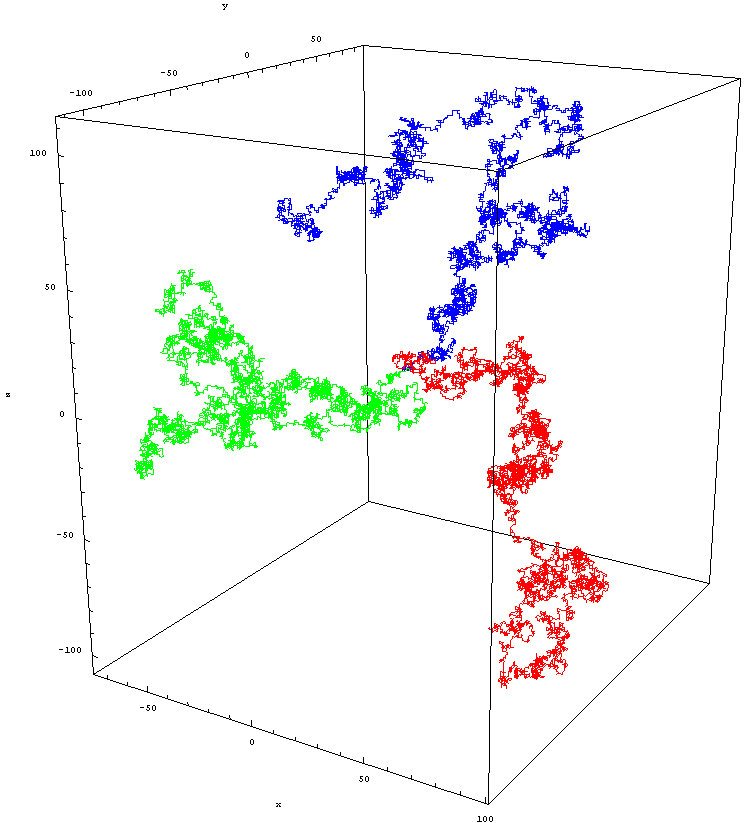
\includegraphics[width=0.744\textwidth,height=0.823\textwidth]{Walk3d_0.png}
\end{center}
\caption{The underlying model for a polymer chain is an
isotropic random walk on the euclidean lattice $\mathbb{Z}^3$.
This picture shows three different walks after 10 000 unit steps,
all three starting from the origin. \label{fig:RandomWalk3D}}
\end{figure}

Consider a flexible polymer coil where each monomer located at a
distance $\mathbf{R}_m$ its scattering field amplitude is given by
\begin{align}
F(\mathbf{q},t) &= \sum_{m=1}^N e^{-\imath
\mathbf{q}\cdot\mathbf{R}_m(t)} .
\end{align}
The scattering intensity averaged over all molecule configurations
reads
\begin{align}
\left\langle \abs{F(\mathbf{q})}^2\right\rangle
&= \sum_{m,n} \left\langle e^{-\imath\mathbf{q}\cdot(\mathbf{R}_m-\mathbf{R}_n)} \right\rangle
\end{align}
As the monomer segments $\mathbf{R}_m-\mathbf{R}_n$ are Gaussian distributed
the averages $\langle\cdots\rangle$ can be written as
\begin{subequations}
\begin{align}
\left\langle e^{-\imath\mathbf{q}\cdot(\mathbf{R}_m-\mathbf{R}_n)} \right\rangle
&= e^{\frac{q^2}{6}\left\langle \left( \mathbf{R}_m-\mathbf{R}_n\right)^2\right\rangle} \\
&= e^{-\frac{q^2b^2}{6}\abs{m-n}^{2\nu}}
\end{align}
\end{subequations}
Here $b$ is the statistical segment length and the contour length $L$ equals $L=Nb$.
The average of the segment inter-distances squares is kept in the general form
\begin{align}
\left\langle \left( \mathbf{R}_m-\mathbf{R}_n\right)^2\right\rangle
&= b^2 \abs{m-n}^{2\nu}.
\end{align}
$\nu$ is the excluded volume parameter from the Flory mean field
theory\footnote{P.J. Flory, "Statistical Mechanics of Chain Molecules", Interscience Publishers (1969)}\footnote{\href{http://www.ncnr.nist.gov/staff/hammouda/the_SANS_toolbox.pdf}{Boualem Hammouda, \texttt{the\_SANS\_toolbox.pdf}}}
of polymer solutions. The radius of gyration $R_G$ is given by
\begin{subequations}
\begin{align}
R_G^2 &= \frac{1}{2N^2}\sum_{m,n}^N \left\langle \left( \mathbf{R}_m-\mathbf{R}_n\right)^2\right\rangle \\
      &= \frac{1}{2N^2}\sum_{m,n}^N b^2 \abs{m-n}^{2\nu} \\
      &= \frac{b^2}{N} \sum_k^N \left(1-\frac{k}{N}\right) k^{2\nu} \\
      &= \frac{b^2}{\left(2\nu+1\right)\left(2\nu+2\right)} N^{2\nu}
\end{align}
\end{subequations}
Three cases are relevant:
\begin{enumerate}
\item Self-avoiding walk corresponds to swollen chains with $\nu = 3/5$, for which
$R_G^2=\frac{25}{176}b^2N^{6/5}$.
\item Pure random walk corresponds to chains in $\Theta$-conditions (where solvent-solvent,
monomer-monomer and solvent-monomer interactions are equivalent) with $\nu = 1/2$,
for which $R_G^2=\frac{1}{6}b^2N$.
\item Self attracting walk corresponds to collapsed chains with $\nu = 1/3$, for which
$R_G^2=\frac{9}{40}b^2N^{2/3}$.
\end{enumerate}
Using the general identity
\begin{align}
\sum_{i,j}^N y(\abs{i-j}) = N+2\sum_{k=1}^N(N-k) y(k)
\end{align}
the form factor reads
\begin{align}
P(q) &= \frac{1}{N^2}\abs{F(q)}^2 = \frac{1}{N^2}
\left\{N+2\sum_{k=1}^N(N-k)e^{-\frac{q^2b^2}{6}k^{2\nu}} \right\}
\end{align}
Going to the continuous limit $(N \gg 1)$, one obtains:
\begin{subequations}
\begin{align}
P(q) &= 2\int_0^1 \mathrm{d}x \; (1-x)e^{-\frac{q^2b^2}{6}N^{2\nu}x^{2\nu}} \\
&= \frac{U^{\frac{1}{2 \nu}} \Gamma\left(\frac{1}{2 \nu}\right)-
\Gamma\left(\frac{1}{\nu}\right)-U^{\frac{1}{2\nu}}
\Gamma\left(\frac{1}{2 \nu},U\right)+\Gamma\left(\frac{1}{\nu},U\right)}{\nu U^{1/\nu}}
\label{eq:generalizedGauss}
\end{align}
\end{subequations}
with the modified variable
\begin{align}
U&=\frac{q^2b^2N^{2\nu}}{6} = \left(2\nu+1\right)\left(2\nu+2\right)\frac{q^2R_G^2}{6}
\end{align}
and the unnormalized incomplete Gamma Function $\Gamma(a,x) = \int_x^\infty \mathrm{d}t \; t^{a-1} \exp(-t)$
for $a$ real and $x \geq 0$ and the Gamma function $\Gamma(a)=\Gamma(a,0)=\int_0^\infty \mathrm{d}t\;  t^{a-1} \exp(-t)$.
Polymer chains follow Gaussian statistics in polymer solutions: they are swollen in good
solvents $\nu=3/5$, are thermally relaxed in "theta"-solvents $\nu=1/2$ and partially precipitate in poor solvents $\nu=1/3$.
The familiar Debye function is recovered when $\nu = 1/2$. The asymptotic limit at large $q$-values of the generalized
Gaussian chain is dominated by the $\frac{1}{\nu U^{\frac{1}{2\nu}}}\Gamma\left(\frac{1}{2\nu}\right)$
term which varies like $U^{-1/(2\nu)} \sim q^{-1/\nu}$. For $\nu =1$ we get the limit of an infinitesimal thin rod
and for $\nu=1/4$ a compact object with a Porod law of $q^{-4}$.

\SASfit has implemented the generalized form of a Gaussian (\texttt{generalized Gaussian coil}) coil and the standard
Debye formula \texttt{Gauss}. In both cases three version are implemented which only differ in their parametrization of
the forward scattering. In case of the the Debye-formula also the polydisperse \texttt{GaussPoly} is implemented.

\textcolor[rgb]{1.00,1.00,1.00}{Gauss}\\
\subsubsection{Gauss \cite{Debye1947}}
\label{sect:Gauss}
~\\
Flexible polymer chains which are not selfavoiding
and obey Gaussian statistics. Debye (1947) has calculated the form factor of such
chains:
\begin{align}
I_\text{Gauss}(q) &= I_0 2\frac{\exp(-u)+u-1}{u^2} \label{eq:DebyeGauss}\\
u &= q^2R_g^2
\end{align}

\vspace{5mm}
\underline{Input Parameters for model \texttt{Gauss}:}
\begin{description}
\item[\texttt{Rg}] radius of gyration $R_g$
\item[\texttt{I0}] forward scattering $I_0$ for $q=0$
\end{description}
\vspace{5mm}

\textcolor[rgb]{1.00,1.00,1.00}{Gauss}\\
\subsubsection{Gauss2 \cite{Debye1947}}
\label{sect:Gauss2}
~\\
This form factor differs only by the parametrization for the forward scattering
$I_0=(b_p-V\eta_\text{s})^2$ from the Debye formula in eq.\ \ref{eq:DebyeGauss}
\begin{align}
I_\text{Gauss2}(q) &= \beta^2 2\frac{\exp(-u)+u-1}{u^2} \\
u &= q^2R_g^2 \nonumber \\
\beta &= b_p-V\eta_\text{s}, \nonumber
\end{align}
where $b_p$ is the scattering length of a polymer molecule of molecular volume $V$ dissolved in a solvent
of scattering length density $\eta_\text{s}$ from which the excess scattering length of a polymer molecule
$\beta$ can be calculated. Combining this form factor with a \texttt{Delta} size distribution \ref{sec:Delta}
is needed to scale the scattering intensity. With proper values for the form factor the parameter $N$
of the \texttt{Delta}-distribution yields the particle number density.

\vspace{5mm}
\underline{Input Parameters for model \texttt{Gauss2}:}
\begin{description}
\item[\texttt{Rg}] radius of gyration $R_g$
\item[\texttt{b\_p}] scattering length of polymer $b_p$ in [cm]
\item[\texttt{V}] molecular volume of a single polymer molecule $V$ in [cm$^3$]
\item[\texttt{eta\_s}] scattering length density of solvent $\eta_\text{s}$ in [cm$^{-1}$]
\end{description}

\textcolor[rgb]{1.00,1.00,1.00}{Gauss}\\
\subsubsection{Gauss3 \cite{Debye1947}}
\label{sect:Gauss3}
~\\
This form factor differs only by the parametrization for the forward scattering
$I_0=(b_p-\frac{M_w}{N_a\rho_p}\eta_\text{s})^2$ from the Debye formula in eq.\ \ref{eq:DebyeGauss}
\begin{align}
I_\text{Gauss3}(q) &= \beta^2 2\frac{\exp(-u)+u-1}{u^2}
\end{align}
with
\begin{align}
u &= q^2R_g^2 \nonumber \\
\beta &= b_p-V\eta_\text{s} \nonumber\\
V &= \frac{M_w}{N_a\rho_p} \nonumber \\
N_a &= \mbox{Avogadro number} \nonumber
\end{align}

\underline{Input Parameters for model \texttt{Gauss3}:}
\begin{description}
\item[\texttt{Rg}] radius of gyration $R_g$
\item[\texttt{b\_p}] scattering length of polymer $b_p$ in [cm]
\item[\texttt{M\_w}] molecular weight of polymer $M_w$ in [g/mol]
\item[\texttt{rho\_p}] mass density of polymer $\rho_p$ in [g cm$^{-3}$]
\item[\texttt{eta\_s}] scattering length density of solvent $\eta_\text{s}$ in [cm$^{-1}$]
\end{description}

\begin{figure}[htb]
\begin{center}
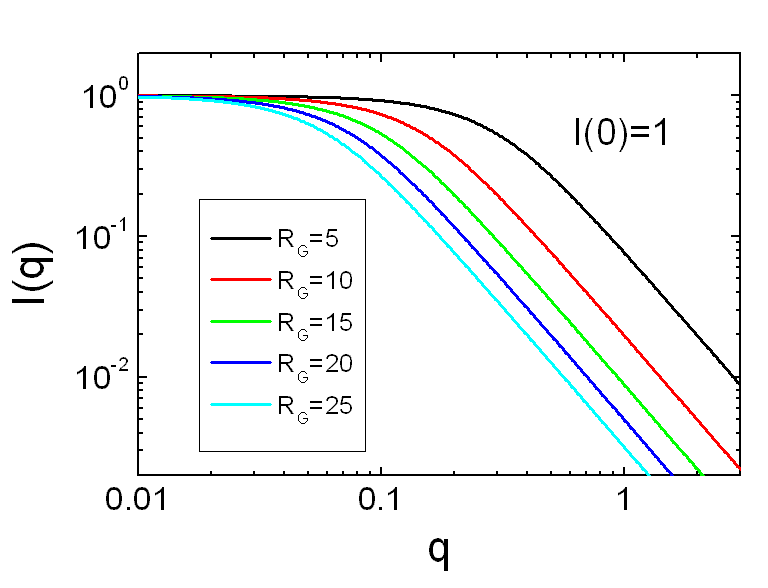
\includegraphics[width=0.768\textwidth,height=0.588\textwidth]{gaussian_coils.png}
\end{center}
\caption{Scattering function of Gaussian coils plotted for several radii of gyration.}
\label{fig:I_gaussian_coils}
\end{figure}

\textcolor[rgb]{1.00,1.00,1.00}{Gauss}\\
\subsubsection{Polydisperse flexible polymers with Gaussian statistics \cite{Pedersen2002}}  \label{sect:GaussPoly}
~\\
Polydispersity has been included in terms of a Schulz�Zimm mass distribution by
Zimm (1948) \cite{zimm:1093}  and Greschner (1973) \cite{Greschner1973}
~\\

\begin{align}
I_\text{GaussPoly}(q) &= I_0 2 \frac{\left( 1+U x\right)^{-1/U}+x-1}{(1+U)x^2} \\
x &= q^2R_g^2/(1+2U) \nonumber \\
U &= \frac{M_w}{M_n} -1 \nonumber
\end{align}

\vspace{5mm}
\underline{Input Parameters for model \texttt{GaussPoly}:}
\begin{description}
\item[\texttt{Rg}] radius of gyration $R_g$
\item[\texttt{M\_w}] weight averaged molecular weight $M_w$
\item[\texttt{M\_n}] number averaged molecular weight $M_n$
\item[\texttt{I0}] forward scattering $I_0$ for $q=0$
\end{description}

\begin{figure}[htb]
\begin{center}
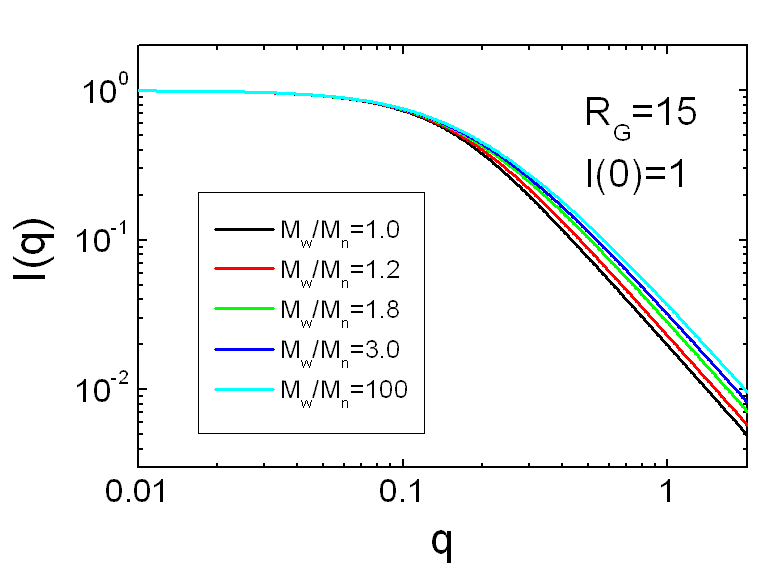
\includegraphics[width=0.768\textwidth,height=0.588\textwidth]{gauss_poly.png}
\end{center}
\caption{Scattering function of polydisperse Gaussian coil plotted for several ratios of $M_w/M_n$.}
\label{fig:I_gauss_poly}
\end{figure}

\textcolor[rgb]{1.00,1.00,1.00}{Gauss}\\
\subsubsection{generalalized Gaussian coil \cite{Hammouda}}
\label{sect:generalized_gaussian_coil}
~\\
The scattering function for the generalized Gaussian coil is according to eq.\ \ref{eq:generalizedGauss}
\begin{align}
I_\text{gGc}(q) &= I_0\frac{U^{\frac{1}{2 \nu}} \Gamma\left(\frac{1}{2 \nu}\right)-
\Gamma\left(\frac{1}{\nu}\right)-U^{\frac{1}{2\nu}}
\Gamma\left(\frac{1}{2 \nu},U\right)+\Gamma\left(\frac{1}{\nu},U\right)}{\nu U^{1/\nu}}
\label{eq:generalizedGauss1}
\end{align}
with the modified variable
\begin{align}
U&= \left(2\nu+1\right)\left(2\nu+2\right)\frac{q^2R_G^2}{6}
\end{align}
and the unnormalized incomplete Gamma Function $\Gamma(a,x) = \int_x^\infty \mathrm{d}t \; t^{a-1} \exp(-t)$
and the Gamma function $\Gamma(a)=\Gamma(a,0)=\int_0^\infty \mathrm{d}t\;  t^{a-1} \exp(-t)$.
$\nu$ is the excluded volume parameter from the Flory mean field theory and typical values for them are
\begin{description}
\item[$\nu=1/3$] partially precipitate in poor solvents
\item[$\nu=1/2$] thermally relaxed in "theta"-solvents
\item[$\nu=3/5$] swollen in good solvents
\end{description}

\vspace{5mm}
\underline{Input Parameters for model \texttt{generalized Gaussian coil}:}
\begin{description}
\item[\texttt{Rg}] radius of gyration $R_g$
\item[\texttt{nu}] excluded volume parameter $\nu\in [1/2;1]$
\item[\texttt{I0}] forward scattering $I_0$ for $q=0$
\end{description}
\vspace{5mm}


\subsubsection{generalized Gaussian coil 2 \cite{Hammouda}}
\label{sect:generalized_gaussian_coil2}
~\\
The scattering function for the generalized Gaussian coil is according to eq.\ \ref{eq:generalizedGauss}
and differs only by the parametrization for the forward scattering
$I_0=(b_p-V\eta_\text{s})^2$ from the formula in eq.\ \ref{eq:generalizedGauss1}
\begin{align}
I_\text{gGc2}(q) &= \left(b_p-V\eta_\text{s}\right)^2\frac{U^{\frac{1}{2 \nu}} \Gamma\left(\frac{1}{2 \nu}\right)-
\Gamma\left(\frac{1}{\nu}\right)-U^{\frac{1}{2\nu}}
\Gamma\left(\frac{1}{2 \nu},U\right)+\Gamma\left(\frac{1}{\nu},U\right)}{\nu U^{1/\nu}}
\label{eq:generalizedGauss2}
\end{align}
with the modified variable
\begin{align}
U&= \left(2\nu+1\right)\left(2\nu+2\right)\frac{q^2R_G^2}{6}
\end{align}

\vspace{5mm}
\underline{Input Parameters for model \texttt{generalized Gaussian coil 2}:}
\begin{description}
\item[\texttt{Rg}] radius of gyration $R_g$
\item[\texttt{b\_p}] scattering length of polymer $b_p$ in [cm]
\item[\texttt{V}] molecular volume of a single polymer molecule $V$ in [cm$^3$]
\item[\texttt{eta\_s}] scattering length density of solvent $\eta_\text{s}$ in [cm$^{-1}$]
\end{description}
\vspace{5mm}

\subsubsection{generalized Gaussian coil 3 \cite{Hammouda}}
\label{sect:generalized_gaussian_coil3}
~\\
The scattering function for the generalized Gaussian coil is according to eq.\ \ref{eq:generalizedGauss}
and differs only by the parametrization for the forward scattering
$I_0=(b_p-\frac{M_w}{N_a\rho_p}\eta_\text{s})^2$ from the formula in eq.\ \ref{eq:generalizedGauss1}
\begin{align}
I_\text{gGc3}(q) &= \left(b_p-\frac{M_w}{N_a\rho_p}\eta_\text{s}\right)^2\frac{U^{\frac{1}{2 \nu}} \Gamma\left(\frac{1}{2 \nu}\right)-
\Gamma\left(\frac{1}{\nu}\right)-U^{\frac{1}{2\nu}}
\Gamma\left(\frac{1}{2 \nu},U\right)+\Gamma\left(\frac{1}{\nu},U\right)}{\nu U^{1/\nu}}
\label{eq:generalizedGauss3}
\end{align}
with the modified variable
\begin{align}
U&= \left(2\nu+1\right)\left(2\nu+2\right)\frac{q^2R_G^2}{6}
\end{align}

\vspace{5mm}
\underline{Input Parameters for model \texttt{generalized Gaussian coil 3}:}
\begin{description}
\item[\texttt{Rg}] radius of gyration $R_g$
\item[\texttt{b\_p}] scattering length of polymer $b_p$ in [cm]
\item[\texttt{M\_w}] molecular weight of polymer $M_w$ in [g/mol]
\item[\texttt{rho\_p}] mass density of polymer $\rho_p$ in [g cm$^{-3}$]
\item[\texttt{eta\_s}] scattering length density of solvent $\eta_\text{s}$ in [cm$^{-1}$]
\end{description}
\vspace{5mm}

\begin{figure}[htb]
\begin{center}
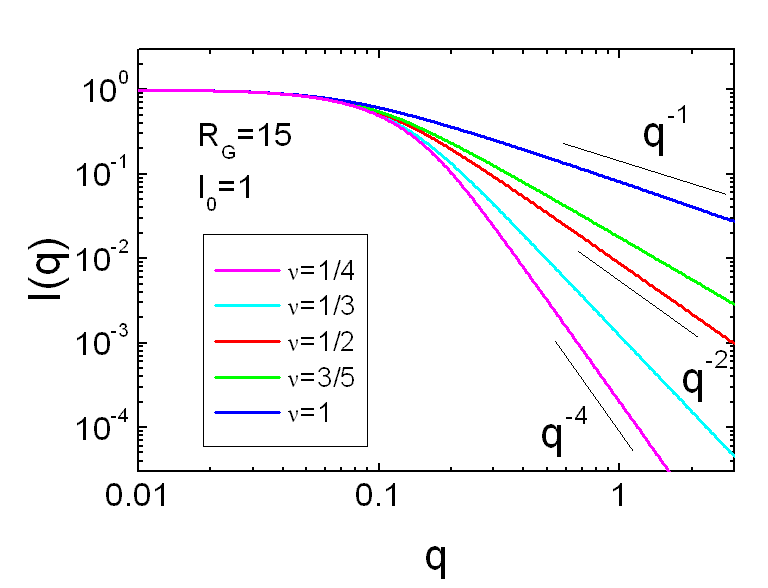
\includegraphics[width=0.768\textwidth,height=0.588\textwidth]{generalized_gaussian_coils.png}
\end{center}
\caption{Scattering function of the generalized Gaussian coil plotted for several excluded volume parameters.}
\label{fig:I_generalized_gaussian_coils}
\end{figure}
\clearpage

\subsection{Star polymer with Gaussian statistic according to
Benoit \cite{Benoit53}}
\label{sect:Benoit}
~\\

\begin{figure}[htb]
\begin{center}
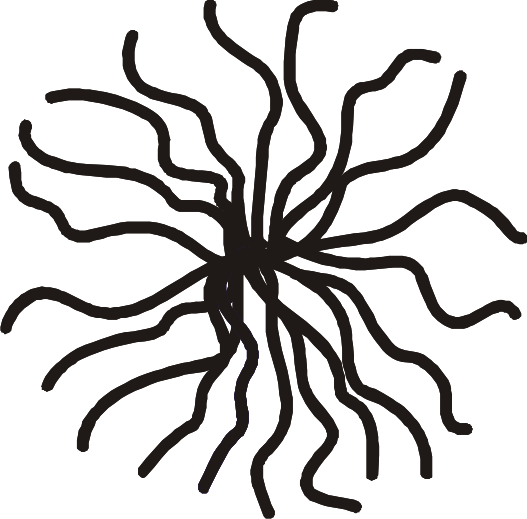
\includegraphics[width=0.2635\textwidth,height=0.2595\textwidth]{Benoit.png}
\end{center}
\caption{Sketch of a branched or star
polymers with $f$ number of arms} \label{fig:BenoitStar}
\end{figure}

Benoit \cite{Benoit53} derived an expression for the scattering from branched or star
polymers with a number of arms $f$, which can be expressed in the following way:
\begin{align}
I_\text{Star}(Q,R_G,f)= I_0 \frac{2}{f\nu^2}
    \left( \nu-\left[1-e^{-\nu}\right]+\frac{f-1}{2}\left[1-e^{-\nu}\right]^2\right)
\end{align}
with $\DS u=R_G^2Q^2$, $\DS \nu=\frac{uf}{3f-2}$ and $\DS
\lim_{Q=0}I_\text{Star}(Q,R_G,f)=I_0$. $f$
denotes the number of arms and $R_G$ the Guinier radius of a
single arm.

\vspace{5mm}

\noindent
\underline{Input Parameters for model \texttt{Benoit}:}
\begin{description}
\item[\texttt{RG}] radius of gyration of the star polymer $R_g$
\item[\texttt{f}] number of arms $f$
\item[\texttt{I0}] forward scattering $I_0$ for $q=0$
\end{description}


\begin{figure}[htb]
\begin{center}
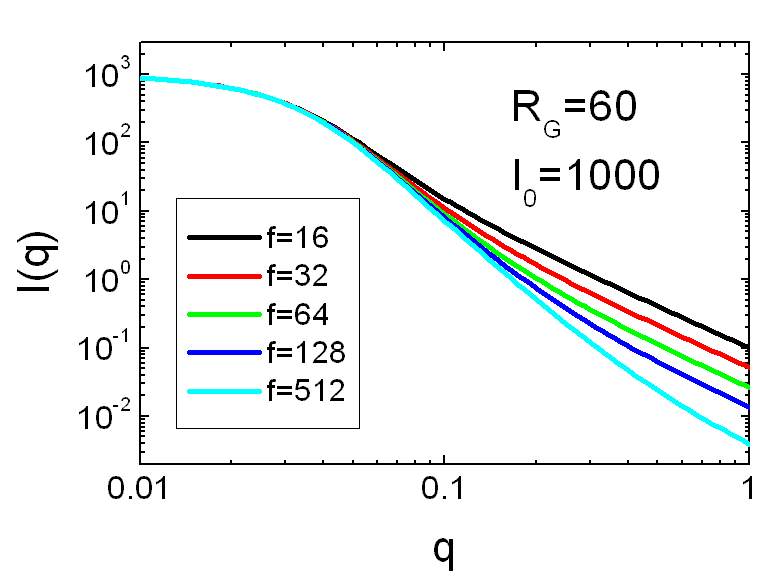
\includegraphics[width=0.768\textwidth,height=0.588\textwidth]{Benoit_Iq.png}
\end{center}
\caption{Scattering function of a star polymer according to Benoit. } \label{fig:Benoit_Iq}
\end{figure}

\clearpage

%\noindent REFERENCE:\\
%H.Benoit, J.Polym.Sci. 11(1953)507 \\


%%%%%%%%%%%%%%%%%%%%%%%%%%%%%%%%%%%%%%%%%%%%%%%%%%%%%%%%%%%%%%%%%%%%%

\subsection{Polydisperse star polymer with Gaussian statistics \cite{burchard74}}
\label{sect:PolydisperseStar}
~\\
\begin{figure}[htb]
\begin{center}
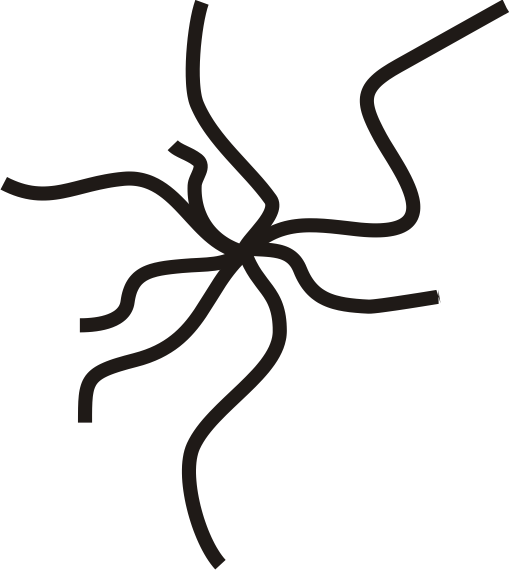
\includegraphics[width=0.2545\textwidth,height=0.2535\textwidth]{polyBenoit.png}
\end{center}
\caption{Polydisperse star polymer with Gaussian statistics} \label{fig:polyBenoitStar}
\end{figure}

For a Schulz�Flory (most probable) distribution (Schulz�Zimm distribution
with $z = 1$) for the mass distribution of the arms, Burchard \cite{burchard74} has given the form factor:
\begin{align}
I_\text{PolydisperseStar}(Q) &= I_0
\frac{1+\frac{u^2}{3 f}}{\left(1+\frac{u^2(f +1)}{6 f }\right)^2}
\end{align}
where $f$ is the number of arms and $u^2 = \langle R_g^2 \rangle_z \,Q^2$, where
$\langle R_g^2 \rangle_z$ is the $z$-average radius of gyration squared of an arm.

\vspace{5mm}

\noindent
\underline{Input Parameters for model \texttt{PolydisperseStar}:}
\begin{description}
\item[\texttt{R\_G}] radius of gyration $R_G$
\item[\texttt{f}] number of arms $f$
\item[\texttt{I0}] forward scattering $I_0$
\end{description}


\begin{figure}[htb]
\begin{center}
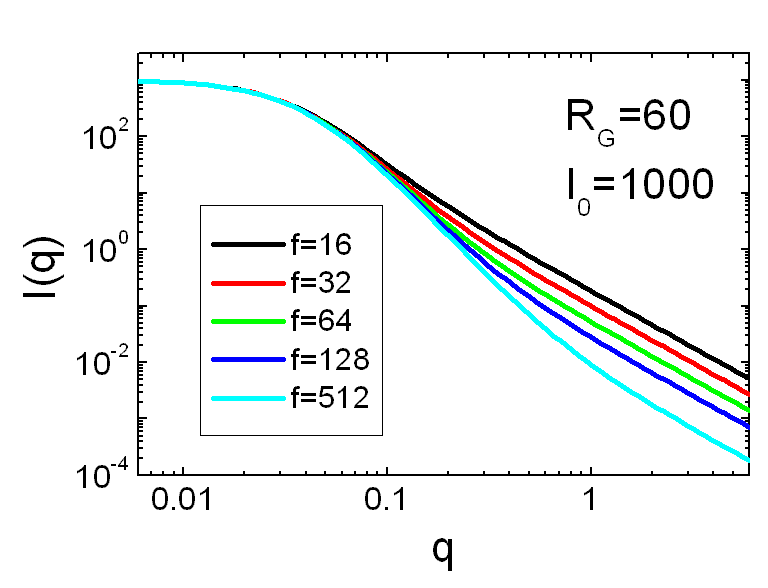
\includegraphics[width=0.768\textwidth,height=0.588\textwidth]{polyBenoit_Iq.png}
\end{center}
\caption{Scattering function of a polydisperse star polymer with Gaussian statistics.} \label{fig:polyBenoit_Iq}
\end{figure}

\clearpage

%%%%%%%%%%%%%%%%%%%%%%%%%%%%%%%%%%%%%%%%%%%%%%%%%%%%%%%%%%%%%%%%%%%%%%%%%%%%%%%%%%%%%%%%

\subsection{Star polymer according to Dozier \cite{dozier91}}
\label{sect:DozierStar}
~\\
\subsubsection{Dozier}
\label{sect:DozierStar1}
~\\
\begin{figure}[htb]
\begin{center}
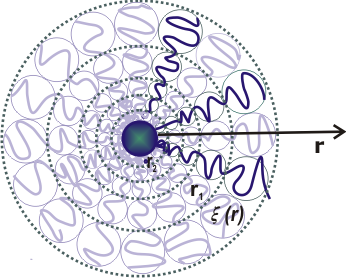
\includegraphics[width=0.346\textwidth,height=0.278\textwidth]{Dozier.png}
\end{center}
\caption{Star polymer according to Dozier} \label{fig:DozierStar}
\end{figure}
Branched polymers having all branches emanating from
the center of the macromolecule are commonly called star
polymers. For a star polymer Dozier \cite{dozier91} has developed
a scattering function which reads:
\begin{align}
I_\text{DozierStar}(Q,I_0,R_G,\alpha,\nu,\xi)
& = I_0 \exp\left(-\frac{Q^2R_G^2}{3}\right) \\
+& \frac{4\pi\alpha}{Q\xi} \Gamma(\mu)
\frac{\sin(\mu\arctan(Q\xi))}{(1+Q^2\xi^2)^{\mu/2}} \nonumber
\end{align}
with $\mu=1/\nu-1$
\begin{align}
R_G      & : \text{radius of gyration} \nonumber \\
I_0      & : \text{scale parameter} \nonumber \\
\alpha   & : \text{scale parameter for fractal term} \nonumber \\
\xi      & : \text{exponential damping length in mass fractal} \nonumber \\
\nu      & : \text{Flory exponent, 3/5 in good solvent, 1/2 in
theta solvent (i.e. $\mu=2/3$ to 1)} \nonumber
\end{align}

\vspace{5mm}

\noindent
\underline{Input Parameters for model \texttt{Dozier}:}
\begin{description}
\item[\texttt{R\_G}] radius of gyration $R_G$
\item[\texttt{I\_0}] scale parameter $I_0$
\item[\texttt{alpha}] scale parameter for fractal term $\alpha$
\item[\texttt{xi}] exponential damping length in mass fractal $\xi$
\item[\texttt{nu}] excluded volume parameter or Flory exponent $\nu$
\end{description}
\vspace{5mm}

\begin{figure}[htb]
\begin{center}
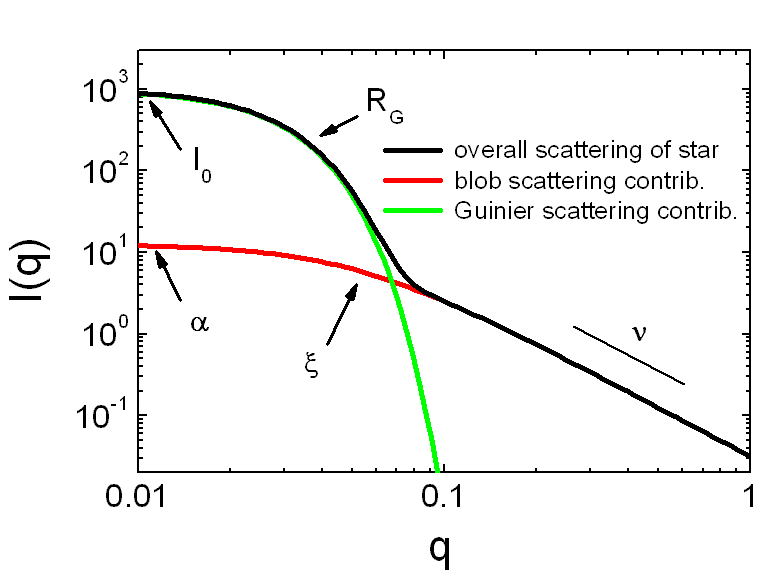
\includegraphics[width=0.768\textwidth,height=0.588\textwidth]{Dozier_Iq.png}
\end{center}
\caption{Scattering function of a star polymer according to Dozier: $I0=10^3$, $R_g=60$, $alpha=1$
$\xi=20$, $\nu=1/2$ } \label{fig:IQDozierStar1}
\end{figure}

\clearpage

\subsubsection{Dozier2}
\label{sect:DozierStar2}
~\\
This is a re-parametrization of the \texttt{Dozier} form factor
to scale the scattering of the overall star to the local scattering of the individual arms.
\begin{align}
I_\text{DozierStar2}(Q,I_0,R_G,N_\text{agg},\nu,\xi)=
\frac{I_0}{N_\text{agg}}
\Biggl(
 &  (N_\text{agg}-1)
    \exp\left(-\frac{Q^2R_G^2}{3}\right) \\
 +&  \frac{\Gamma(\mu)}{Q\xi}
    \frac{\sin(\mu\arctan(Q\xi))}{(1+Q^2\xi^2)^{\mu/2}} \nonumber
\Biggr)
\end{align}
with $\mu=1/\nu-1$
\begin{align}
R_G      & : \text{radius of gyration of the star} \nonumber \\
I_0      & : \text{scale parameter} \nonumber \\
N_\text{agg} & : \text{number of arms in the star} \nonumber \\
\xi      & : \text{exponential damping length in mass fractal} \nonumber \\
\nu      & : \text{Flory exponent, 3/5 in good solvent, 1/2 in
theta solvent (i.e. $\mu=2/3$ to 1)} \nonumber
\end{align}

\vspace{5mm}

\noindent
\underline{Input Parameters for model \texttt{Dozier2}:}
\begin{description}
\item[\texttt{R\_G}] radius of gyration of the star $R_G$
\item[\texttt{I\_0}] scale parameter $I_0$
\item[\texttt{Nagg}]  number of arms $N_\text{agg}$ in the star from which the scale parameter for fractal term is calculated
\item[\texttt{xi}] exponential damping length in mass fractal $\xi$
\item[\texttt{nu}] Flory exponent, $\nu=3/5$ in good solvent, $\nu=1/2$ in
theta solvent (i.e. $\mu=2/3$ to 1)
\end{description}
\vspace{5mm}

\begin{figure}[htb]
\begin{center}
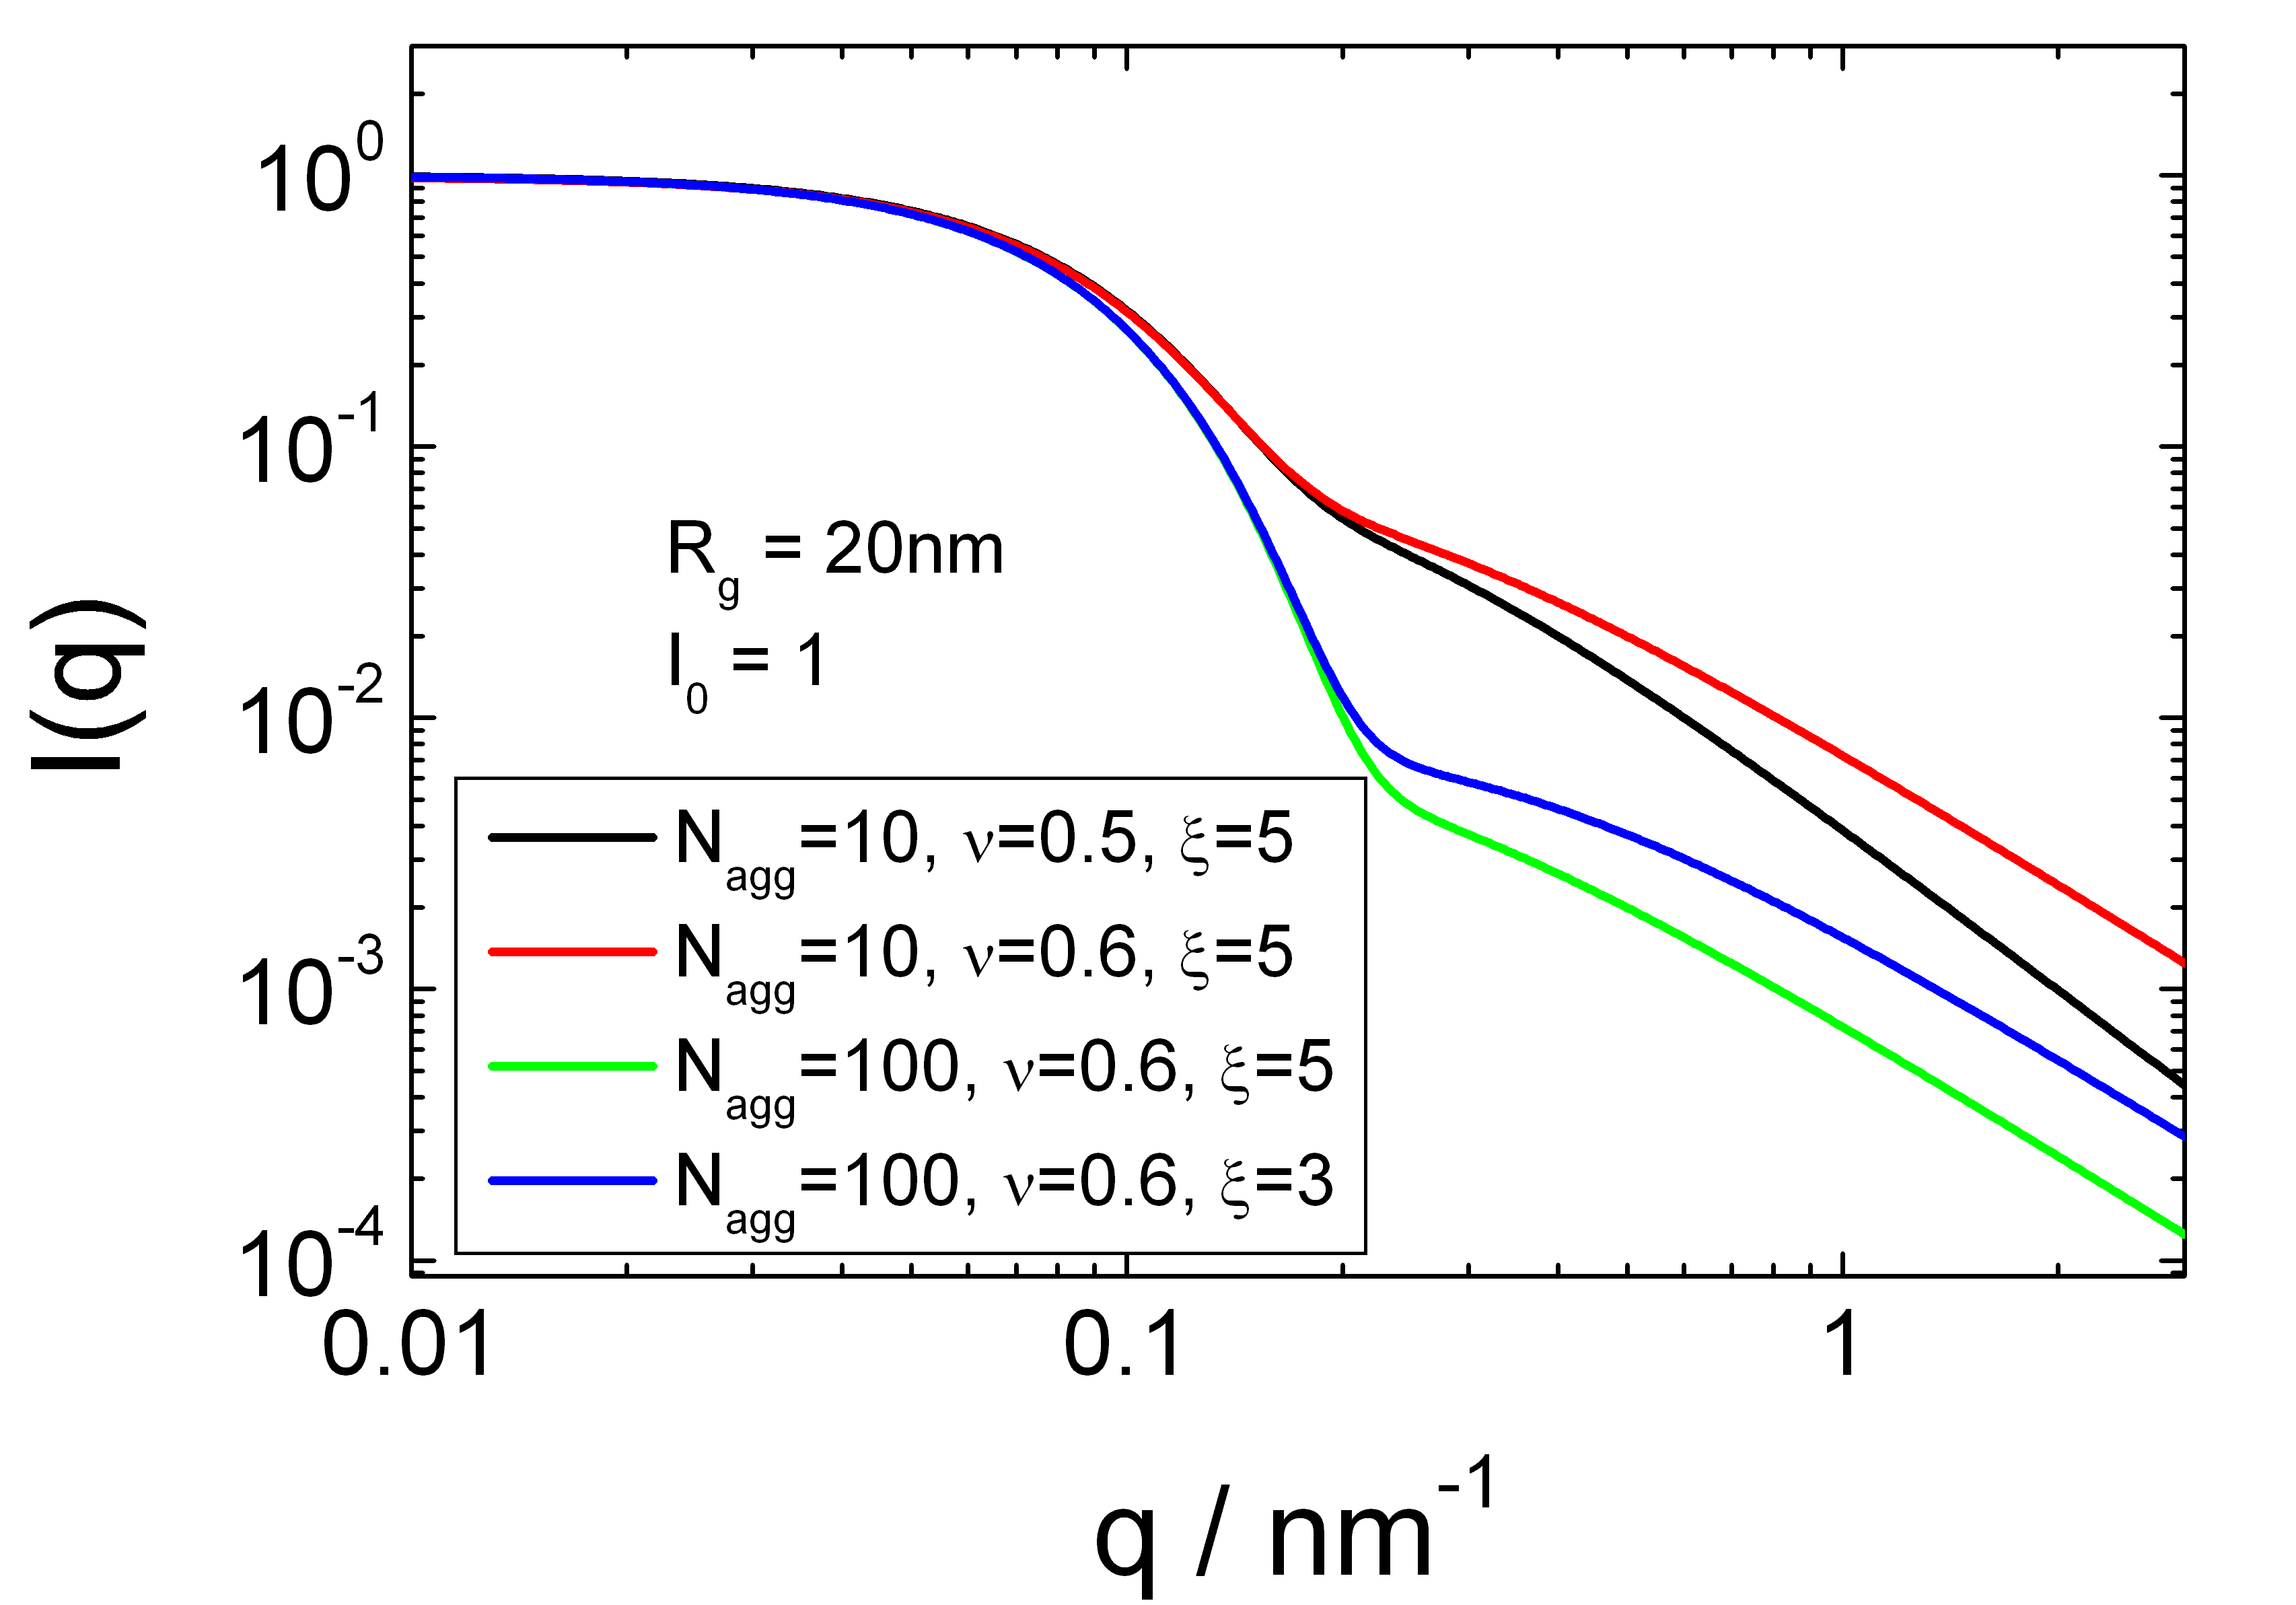
\includegraphics[width=0.768\textwidth,height=0.588\textwidth]{Dozier2_Iq.png}
\end{center}
\caption{Scattering function of a star polymer according to Dozier but modified
to scale the scattering of the overall star to the local scattering of the individual arms
by the number of arms} \label{fig:IQDozierStar2}
\end{figure}
\clearpage

%\noindent REFERENCE:\\
%W.D.Dozier, J.S.Huang \& L.J.Fetters, Macromolecules
%24(1991)2810-2814

%%%%%%%%%%%%%%%%%%%%%%%%%%%%%%%%%%%%%%%%%%%%%%%%%%%%%%%%%%%%%%%%%%%%%%%%


\subsection{Flexible Ring Polymer \cite{Burchard1996}}
\label{sect:FlexibleRingPolymer}
~\\

\begin{figure}[htb]
\begin{center}
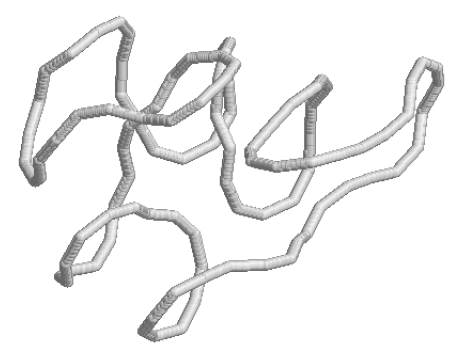
\includegraphics[width=0.471\textwidth,height=0.353\textwidth]{flexibleRing.png}
\end{center}
\caption{Sketch of a flexible ring polymer.}
\label{fig:flexibleRing}
\end{figure}

\begin{align}
P_{1r}(q) & = \sqrt{\frac{2}{u_{1r}^2}} D\left[ \sqrt{\frac{u_{1r}^2}{2}} \right] \\
u_{1r}^2 &= q^2R^2_{g,1r} \\
R^2_{g,1r} &= \sqrt{\frac{b^2N}{12}} \\
D(X) &= \exp\left(X^2\right) \int_0^X \exp(t^2)\, \mathrm{d}t
\end{align}

\vspace{5mm}

\noindent
\underline{Input Parameters for model \texttt{FlexibleRingPolymer}:}
\begin{description}
\item[\texttt{Rg}] radius of gyration $R_G$
\item[\texttt{I0}] forward scattering $I_0$
\end{description}

\begin{figure}[htb]
\begin{center}
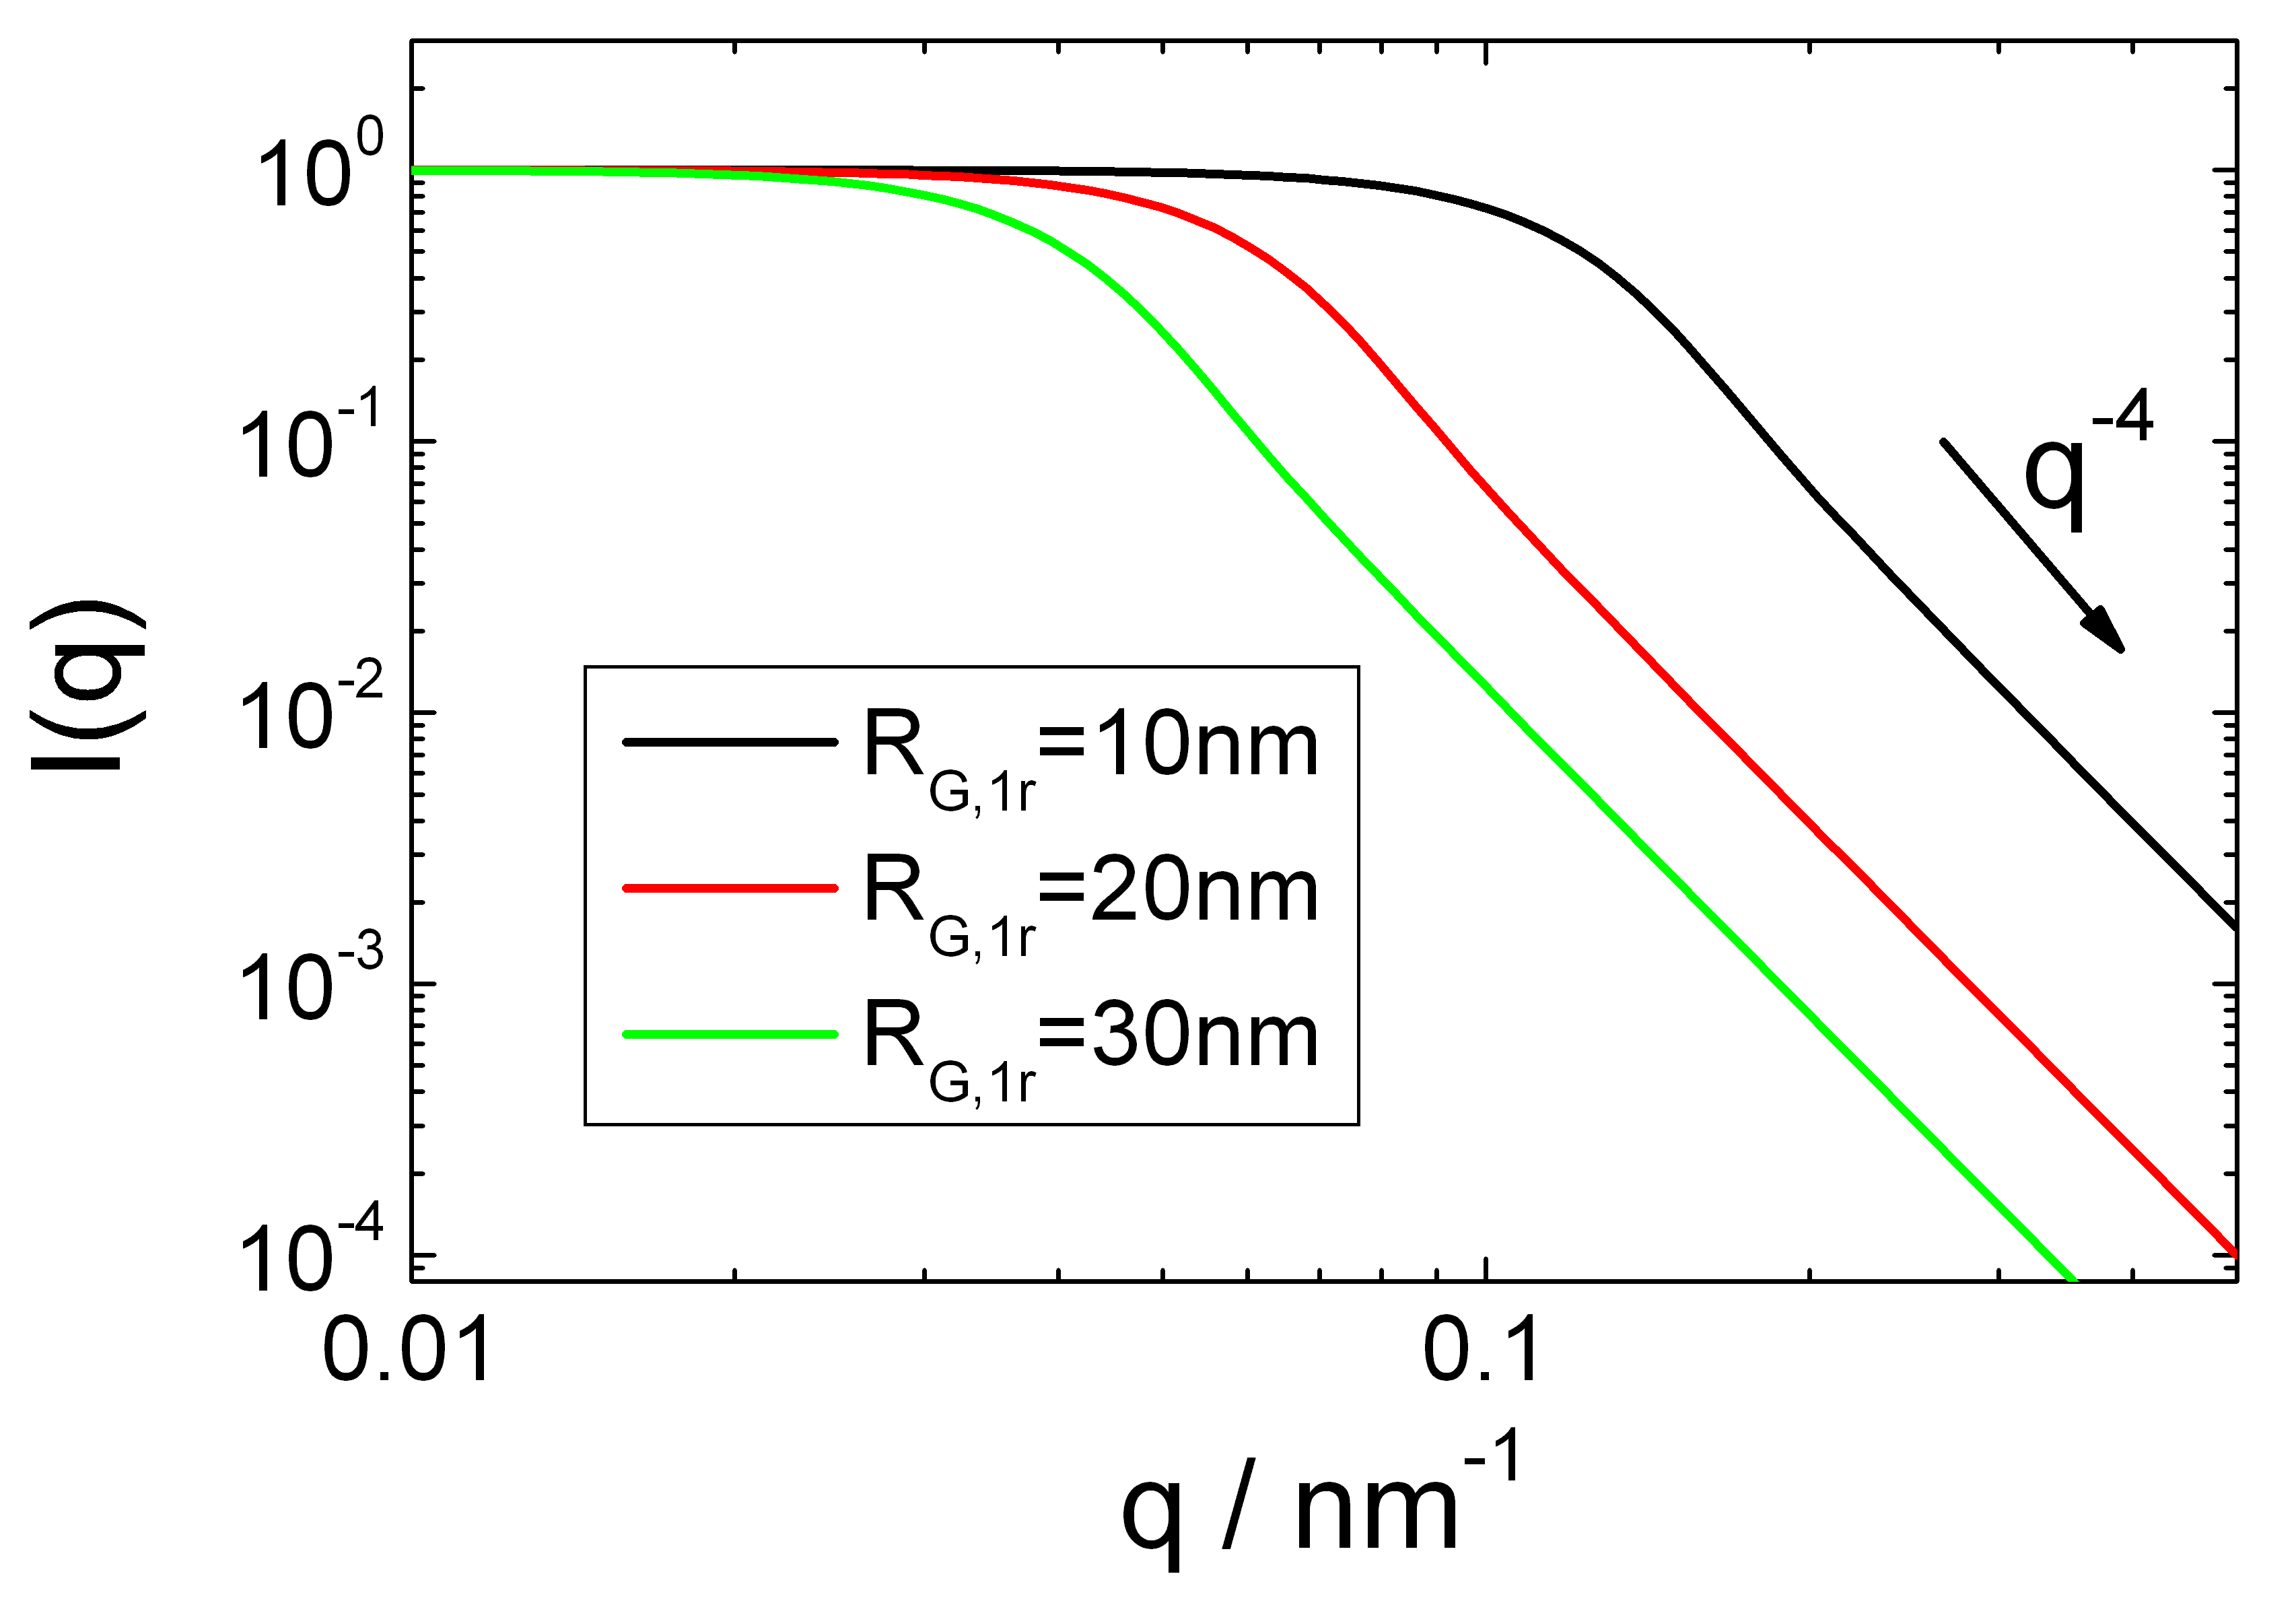
\includegraphics[width=0.768\textwidth,height=0.588\textwidth]{ringIQ.png}
\end{center}
\caption{Scattering intensity of ring polymers of different radius of gyration.} \label{fig:ringIQ}
\end{figure}

%%%%%%%%%%%%%%%%%%%%%%%%%%%%%%%%%%%%%%%%%%%%%%%%%%%%%%%%%%%%%%%%%%%%%%%

\clearpage
\subsection{$m$-membered twisted ring \cite{Burchard1996}}
\label{sect:mMemberedTwistedRing}
~\\
\begin{figure}[htb]
\begin{center}
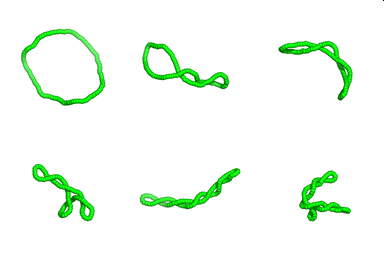
\includegraphics[width=0.768\textwidth,height=0.516\textwidth]{TWsnap.png}
\end{center}
\caption{Sketch of ing polymers which different degree of twisting}
\label{fig:mMemberedTwistedRing}
\end{figure}

\begin{align}
P_{mr}(q) & = I_0\left(\frac{P_{1r}(q)}{m} + \frac{2}{m^2}P_{1r}^2(q)\sum_{j=1}^{m-1}(m-j)\exp\left(-\frac{q^2R^2_{g,1r}}{2}(j-1)\right)\right) \\
P_{1r}(q) & = \sqrt{\frac{2}{u_{1r}^2}} D\left[ \sqrt{\frac{u_{1r}^2}{2}} \right] \\
u_{1r}^2 &= q^2R^2_{g,1r} \\
R^2_{g,1r} &= \sqrt{\frac{b^2N}{12}} \\
D(X) &= \exp\left(X^2\right) \int_0^X \exp(t^2)\, \mathrm{d}t
\end{align}

\vspace{5mm}

\noindent
\underline{Input Parameters for model \texttt{mMemberedTwistedRing}:}
\begin{description}
\item[\texttt{R\_G,1r}] radius of gyration $R_{G,1r}$ of one of $m$ loop
\item[\texttt{m}]  number of twists $m$
\item[\texttt{I0}] forward scattering $I_0$
\end{description}

\begin{figure}[htb]
\begin{center}
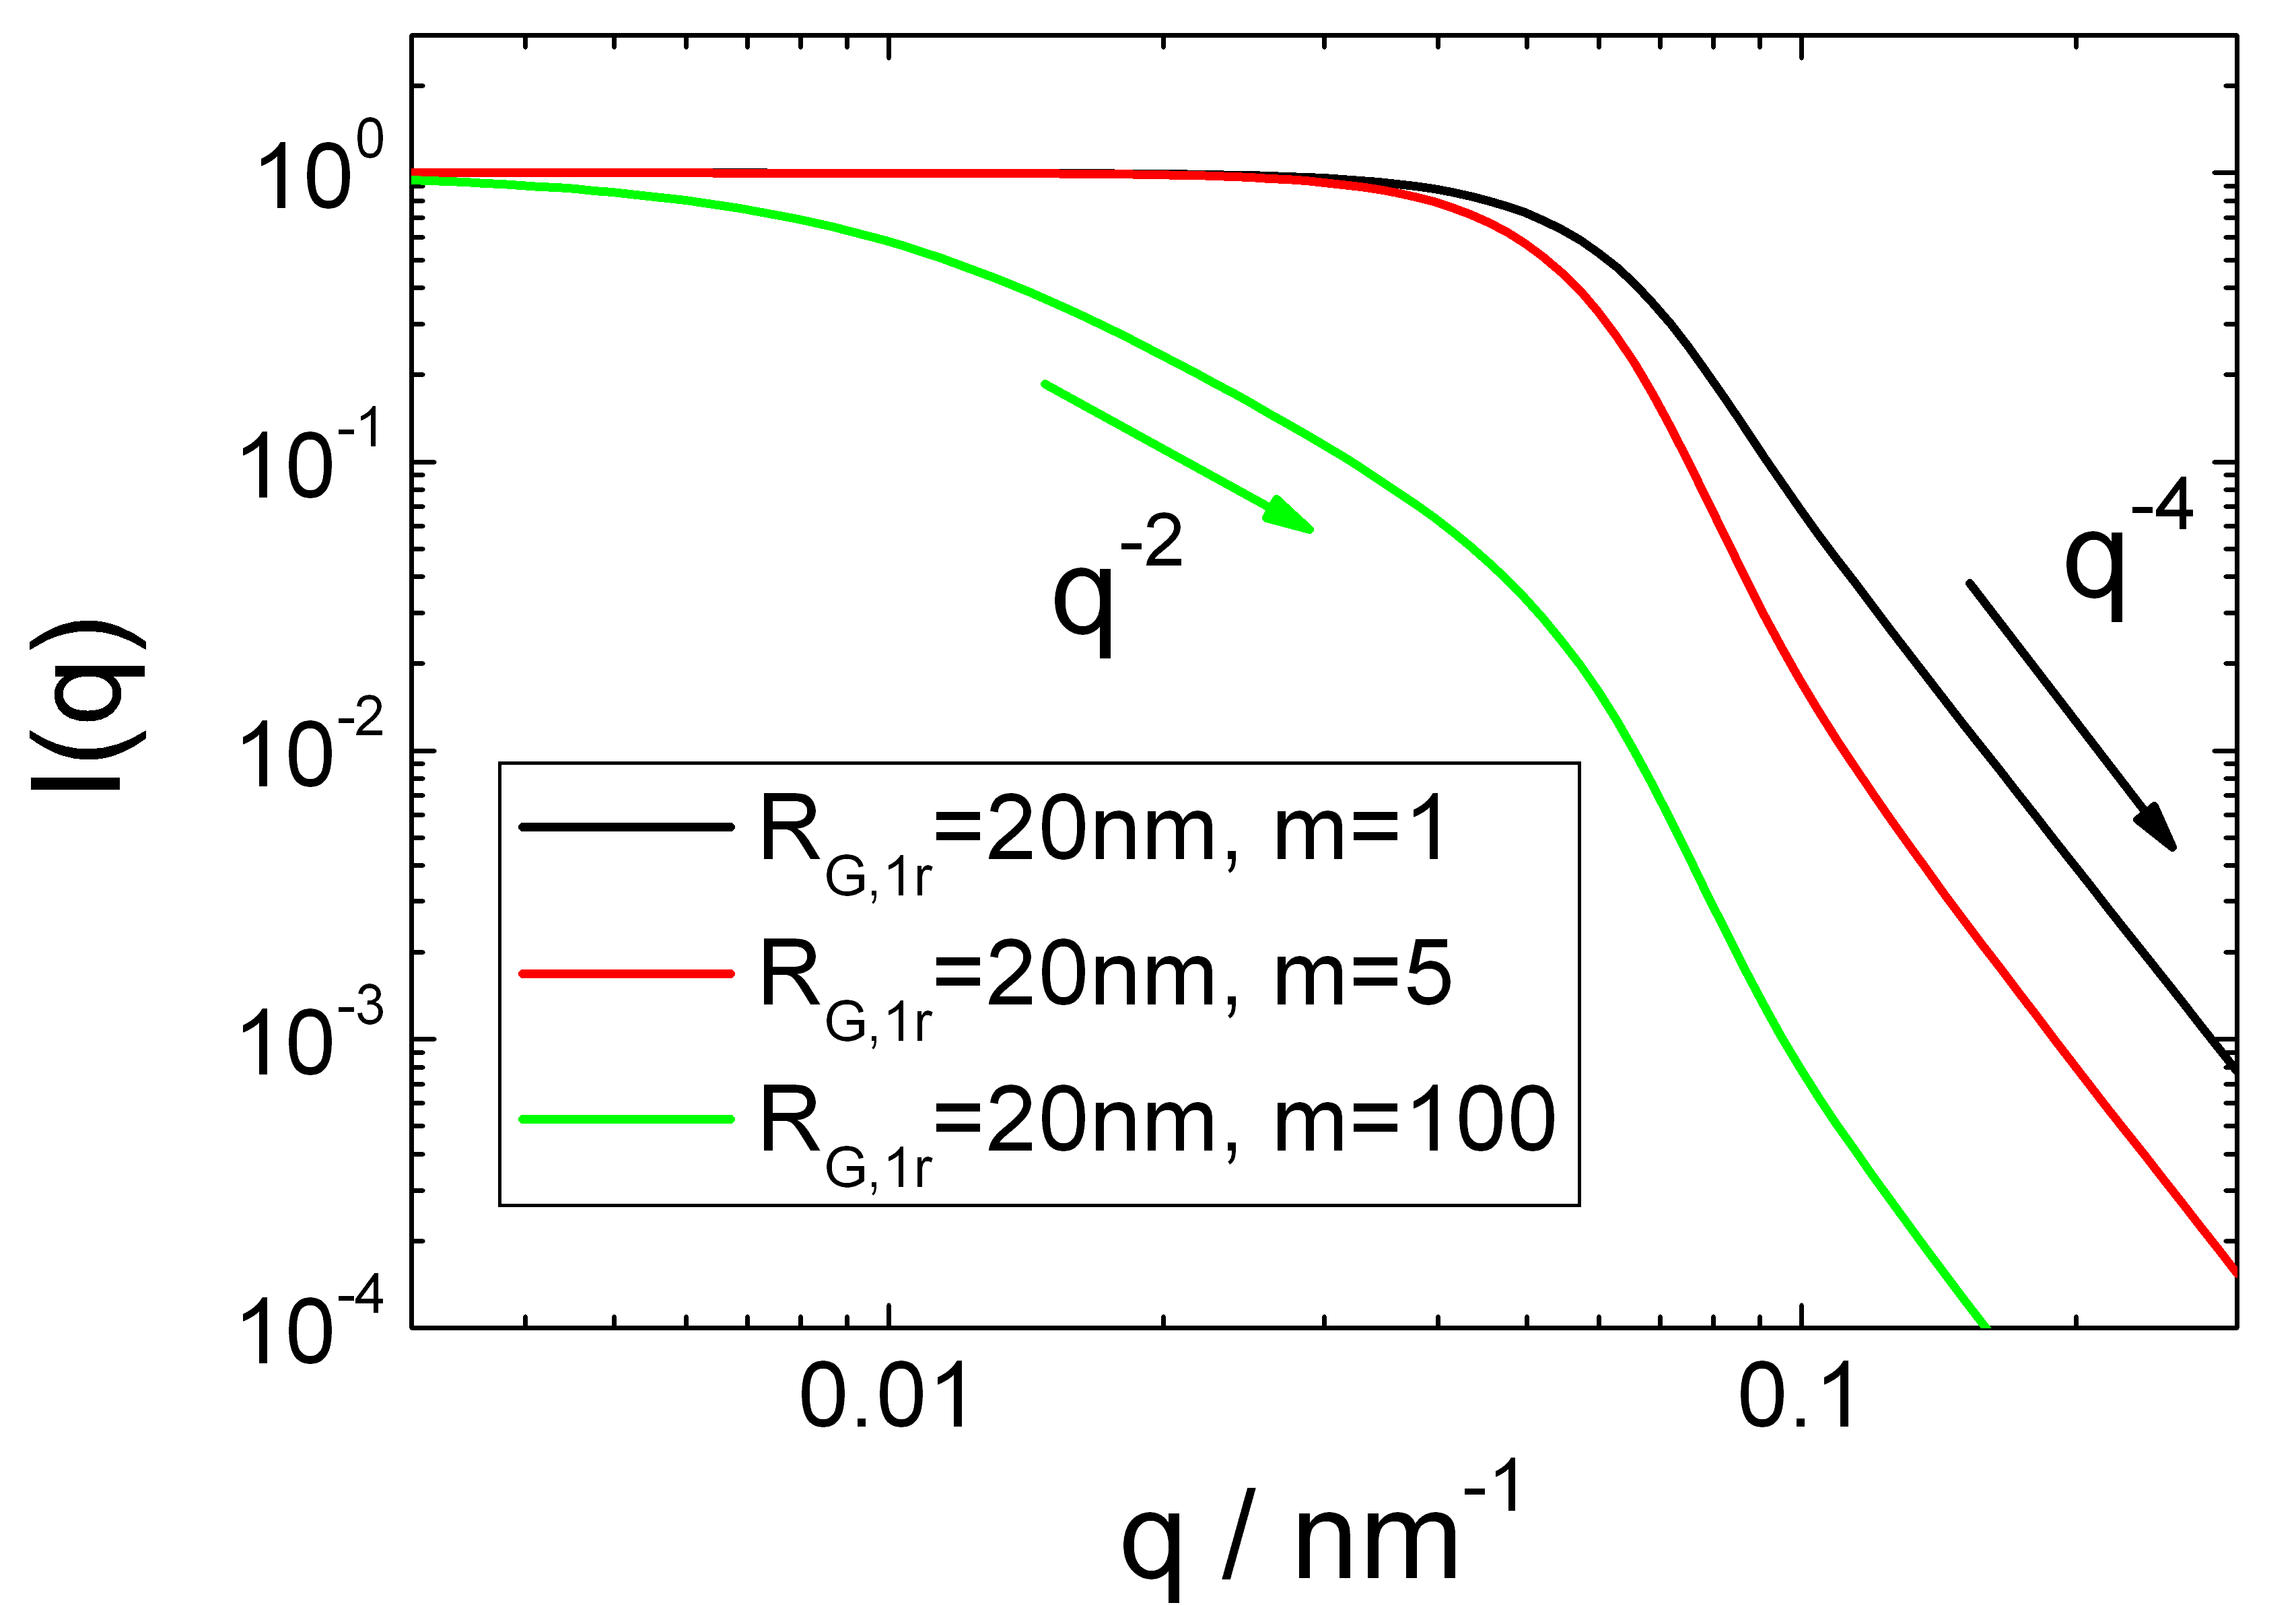
\includegraphics[width=0.768\textwidth,height=0.588\textwidth]{mMemberedTwistedRing.png}
\end{center}
\caption{Scattering intensity of an $m$-membered twisted ring polymers with different values for $m$.} \label{fig:mMemberedTwistedRingIQ}
\end{figure}

%%%%%%%%%%%%%%%%%%%%%%%%%%%%%%%%%%%%%%%%%%%%%%%%%%%%%%%%%%%%%%%%%%%%%%%%

\clearpage
\subsection{Daisy-like Ring \cite{Burchard1996}}
\label{sect:DaisyLikeRing}
~\\
\begin{figure}[htb]
\begin{center}
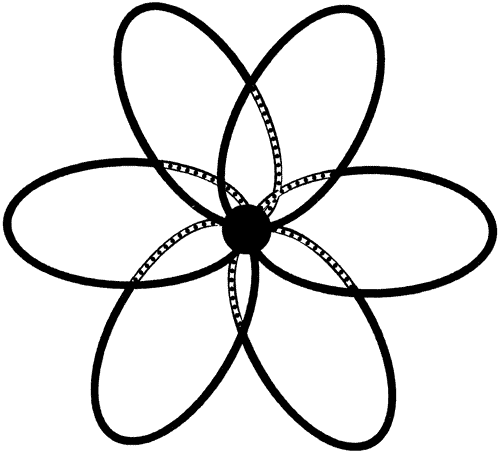
\includegraphics[width=0.5\textwidth,height=0.453\textwidth]{ma9603286f00001.png}
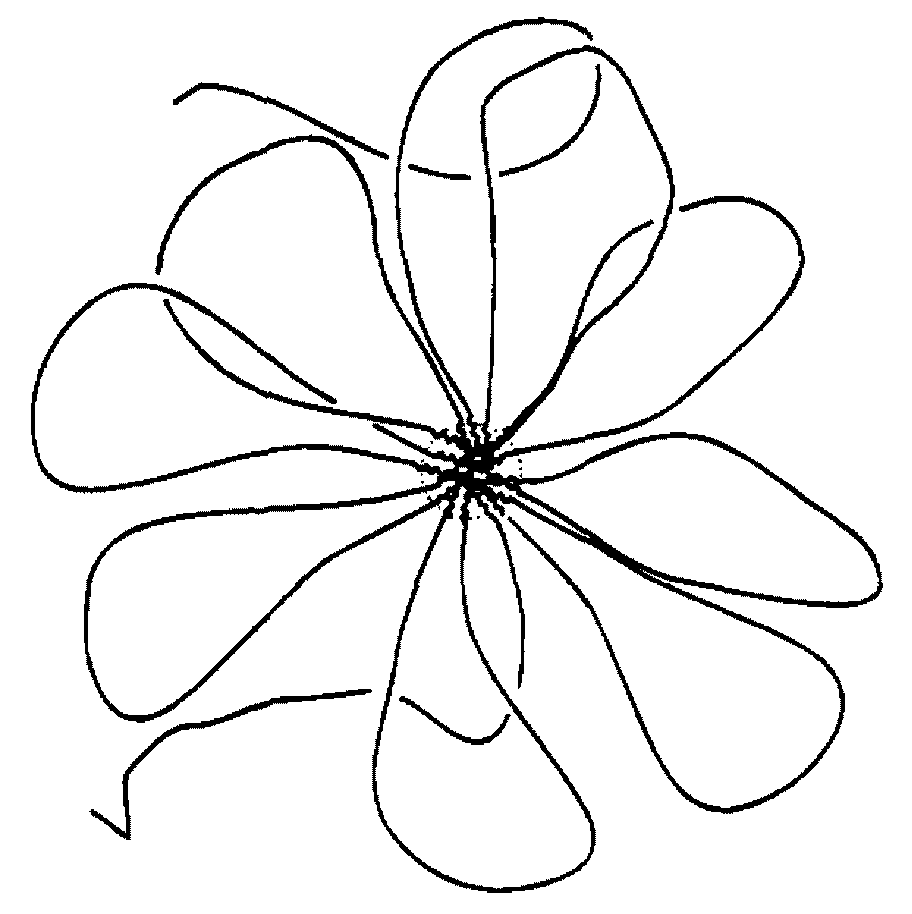
\includegraphics[width=0.45\textwidth,height=0.45\textwidth]{RosetteLikeMicelle.png}
\end{center}
\caption{Sketch of a Daisy-like polymer.}
\label{fig:DaisyLike}
\end{figure}

\begin{align}
P_{mr}(q) & = \frac{I_0}{m}\left(P_{1r}(q) + (m-1)P_{1r}^2(q)\right) \\
P_{1r}(q) & = \sqrt{\frac{2}{u_{1r}^2}} D\left[ \sqrt{\frac{u_{1r}^2}{2}} \right] \\
u_{1r}^2 &= q^2R^2_{g,1r} \\
R^2_{g,1r} &= \sqrt{\frac{b^2N}{12}} \\
D(X) &= exp(X^2) \int_0^X exp(t^2)\, \mathrm{d}t
\end{align}

\vspace{5mm}

\noindent
\underline{Input Parameters for model \texttt{DaisyLikeRing}:}
\begin{description}
\item[\texttt{R\_G,1r}] radius of gyration $R_{G,1r}$ of one of $m$ loop
\item[\texttt{m}]  number of loops $m$
\item[\texttt{I0}] forward scattering $I_0$
\end{description}

\begin{figure}[htb]
\begin{center}
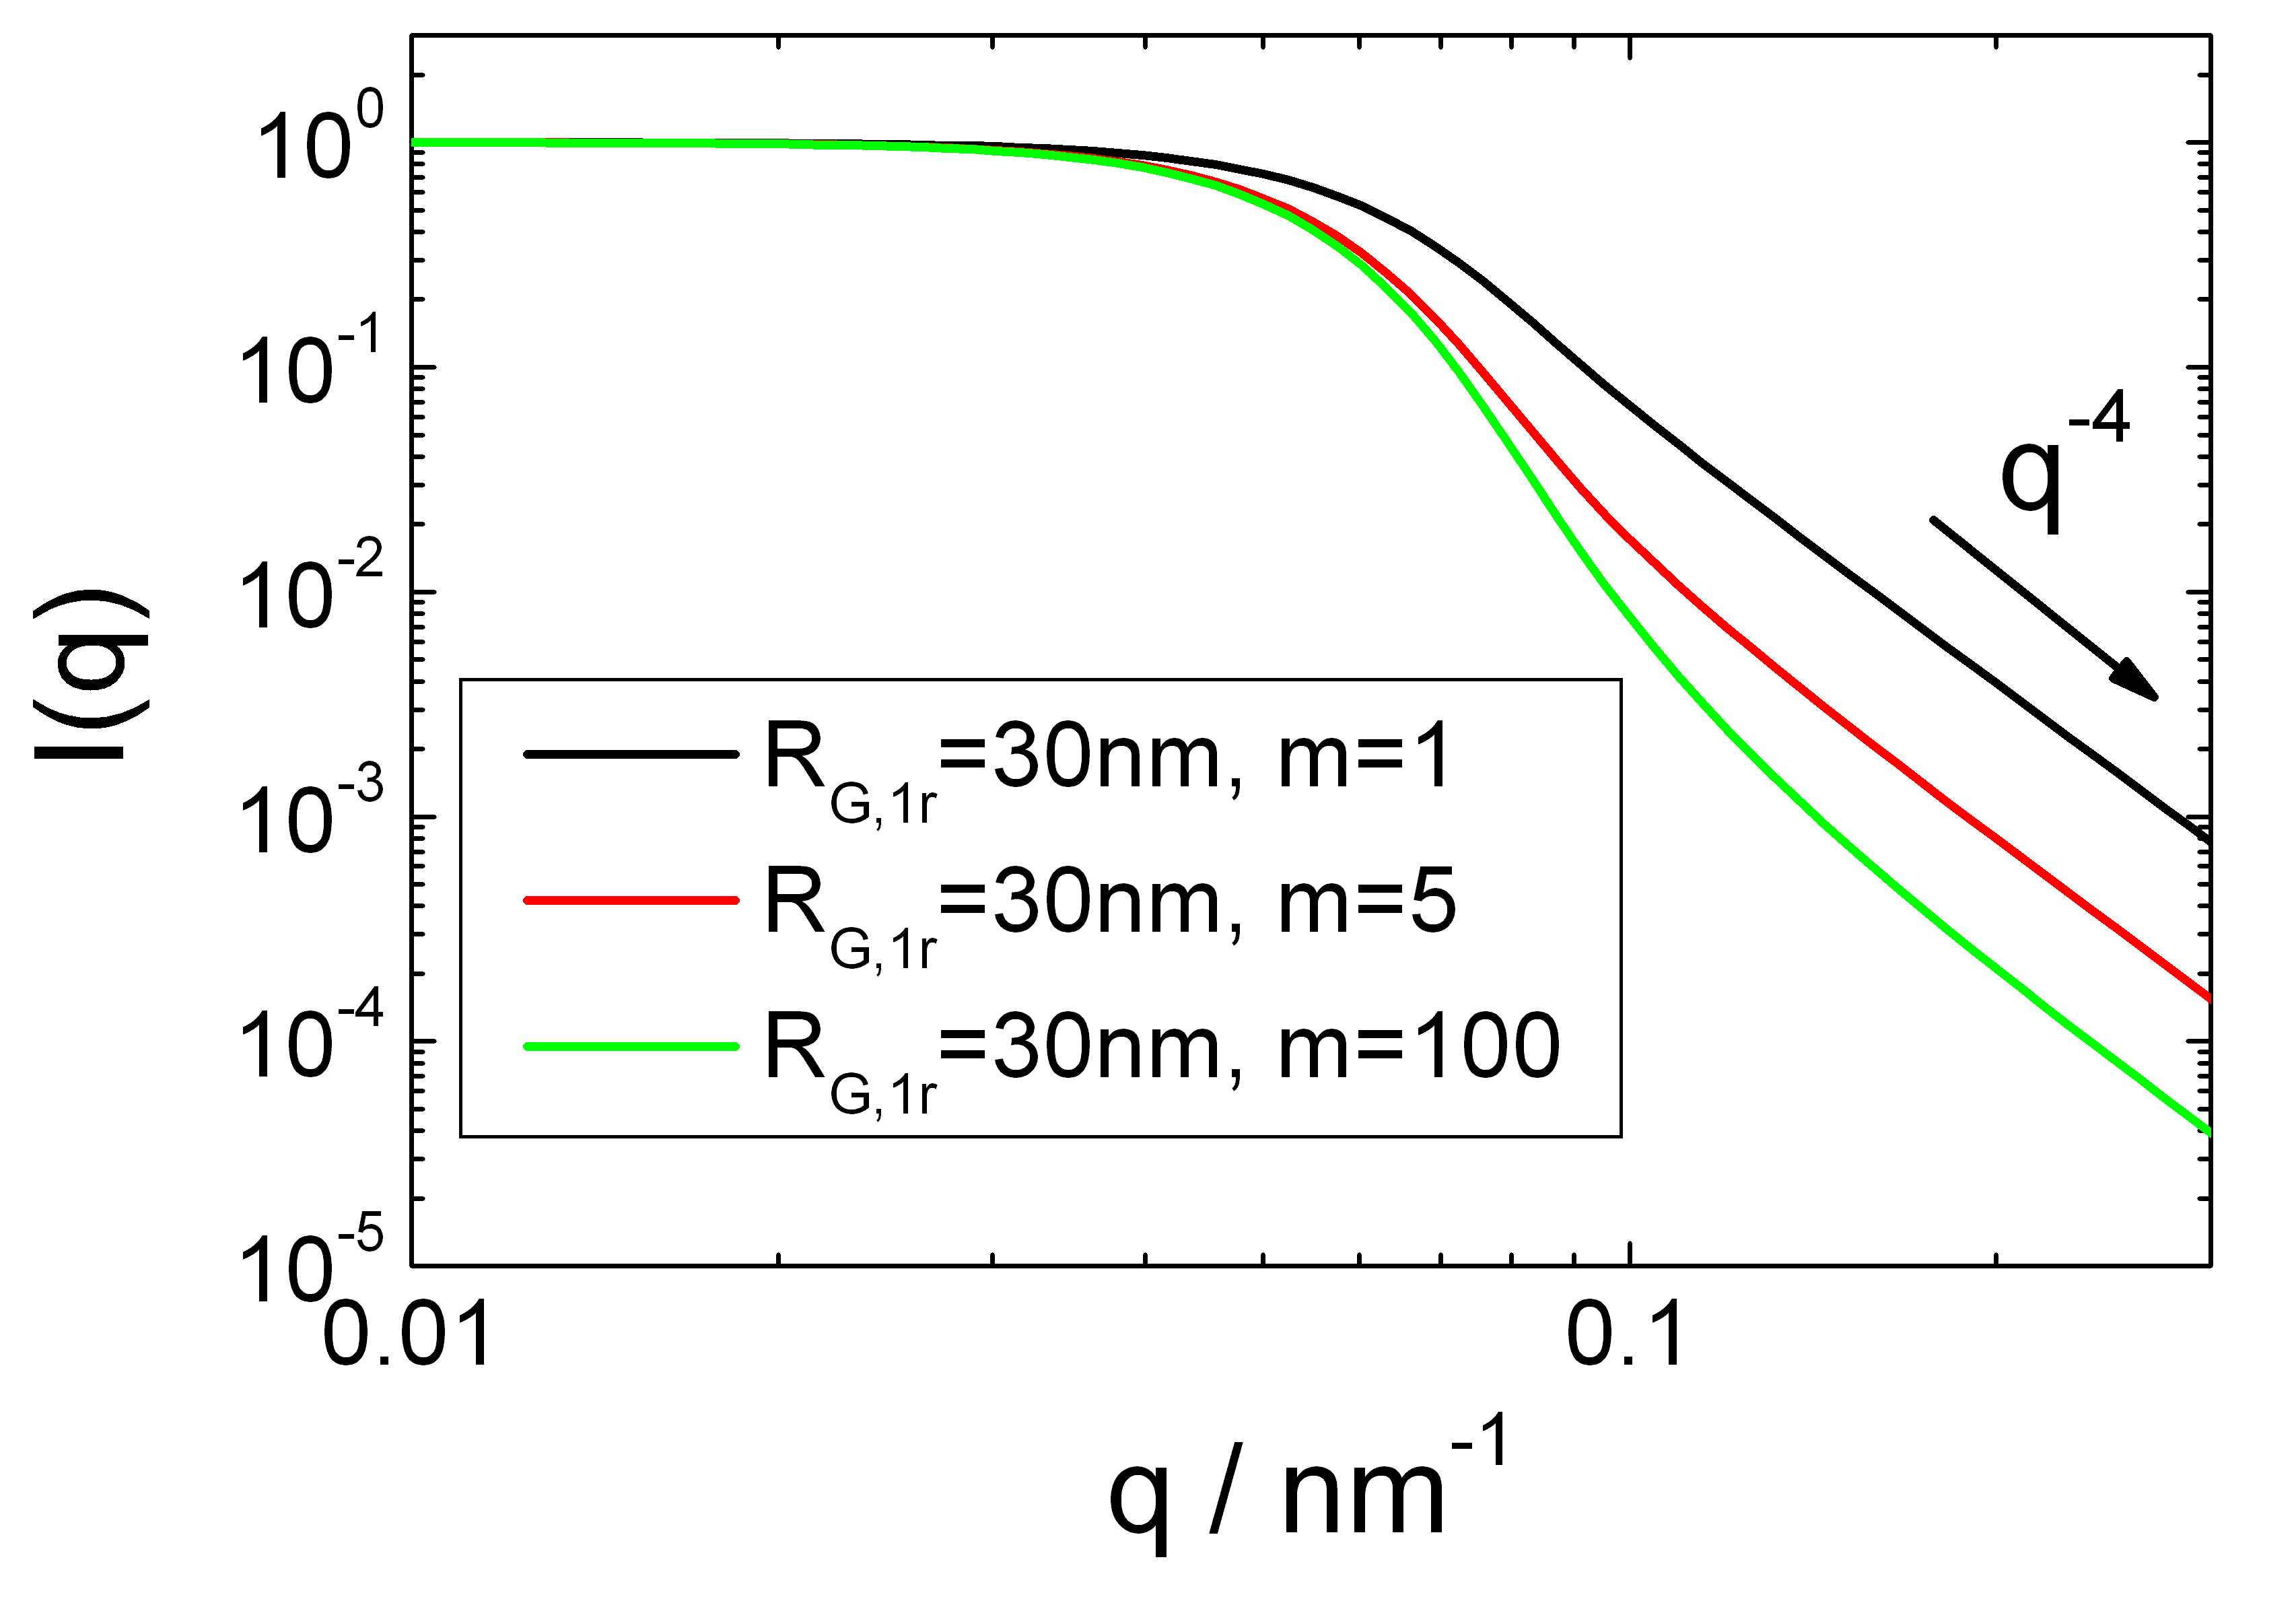
\includegraphics[width=0.768\textwidth,height=0.588\textwidth]{DaisyRingIQ.png}
\end{center}
\caption{Scattering intensity of a Daisy-like ring polymers with different number of loops.} \label{fig:DaisyRingIQ}
\end{figure}
%%%%%%%%%%%%%%%%%%%%%%%%%%%%%%%%%%%%%%%%%%%%%%%%%%%%%%%%%%%%%%%%%%%%%%%

\clearpage

\subsection{Unified Exponential Power Law according to Beaucage \cite{beaucage95,beaucage96}}
\label{sect:Beaucage}
~\\

\begin{figure}[htb]
\begin{center}
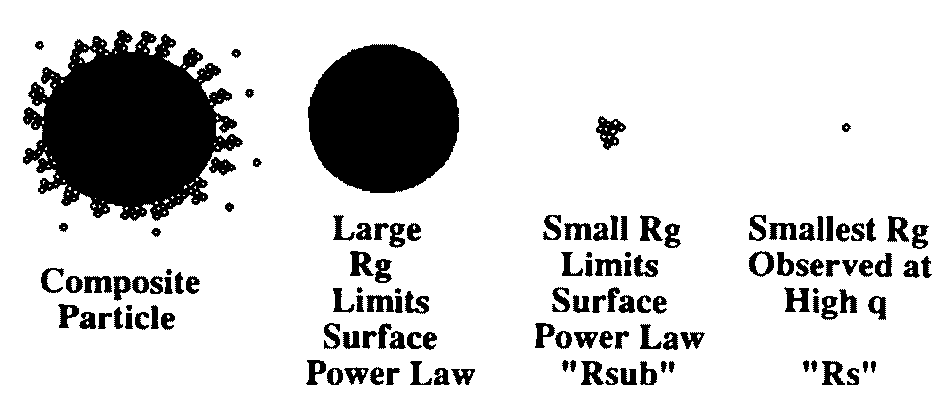
\includegraphics[width=0.952\textwidth,height=0.403\textwidth]{Beaucage.png}
\end{center}
\caption{A typical case in which two $R_g$'s are observed.
Particles composed of sub-particles where a radius of gyration for
the entire particle, $R_g$, and a radius of gyration for the
sub-particles, $R_s$, are observed. The surface-fractal cut-off
radius of gyration, $R_{sub}$, differs from the high-$Q$ radius of
gyration, $R_s$, in this case. Generally, $R_s = R_{sub}$}
\label{Beaucage}
\end{figure}

\subsubsection{Beaucage} ~\\

\begin{align}
\begin{split}
I_\text{Beaucage}(Q) & \simeq
    G \exp\left(-\frac{Q^2R_g^2}{3}\right) \\
& + B \exp\left(-\frac{Q^2R_{sub}^2}{3}\right)
      \left( \frac{\left[\mathrm{erf}\left(QkR_g/\sqrt{6}\right)\right]^3}{Q}\right)^P  \\
& + G_s \exp\left(-\frac{Q^2R_s^2}{3}\right) \\
& + B_s %\exp\left(\frac{-Q^2R_{sub}^2}{3}\right)
      \left( \frac{\left[\mathrm{erf}\left(Qk_sR_s/\sqrt{6}\right)\right]^3}{Q}\right)^{P_s}
\end{split} \label{eq:UEPL}
\end{align}
The first term in eq.\ \ref{eq:UEPL} describes the large-scale
structure of size $R_g$ composed of small subunits of
size $R_s$, captured in the third term. The second term describes
the mass-fractal regime with two structural limits. The low-$Q$
limit is at $R_g$ and is described by the error function. The
high-$Q$ limit is at $R_{sub}$ and is described by the exponential
pre-factor \cite{beaucage95} . The final two terms are for the
sub-structural mer unit. Using eq.\ \ref{eq:UEPL}, scattering from a
system with multiple-size-scale features is parameterized.
Generally, the high-$Q$ cutoff for the intermediate power law,
$R_{sub}$, is identical to the sub-structural radius of gyration,
$R_s$. The assumption that $R_{sub} = R_s$ should always be true
for typical mass fractals. It should be noted that, although eq.\
\ref{eq:UEPL} appears cumbersome, no new parameters have been
introduced over local fits using exponentials and power laws.

$G$ is the Guinier pre-factor defined above and $B$ is a
pre-factor specific to the type of power-law scattering:
$B$ is defined according to the regime in which the exponent
$P$ falls. Generally, for surface fractals $4 > P > 3$,
for mass fractals $P < 3$ and for diffuse interfaces $P>4$.
For Porod's law, $P=4$
and $B = N_p 2\pi \rho_c^2pS_p$, where $S_p$, is the particulate surface
area. For a Gaussian polymer, $P = 2$, and $B$ is given by
$2G/R_g^2$, through a comparison with the Debye form factor \ref{sect:GaussCoil}
at the high-$Q$ limit as discussed below.
The constant, $k$ in \ref{eq:UEPL}, accounts for
an approximation involved in the description of the low-$Q$
power-law limit \cite{beaucage95}. This is an empirical
constant that has a value of 1 for steep power-law decays,
$P > 3$. For weak power-law decays, $k$ deviates slightly
from 1. For polymeric mass fractals of fractal dimension
$d_f$ close to 2 (1.5 to 3), $k$ is empirically found to be close
to 1.06. Weak deviations are observed between the scattered
intensity as calculated using \ref{eq:UEPL} and exact
calculations for values of $Q$ between $2\pi/R_g$ and $\pi/R_g$ in
these cases when $k = 1$. These deviations are reduced to
less than 3\% of the calculated intensity using $k= 1.06$.

\hspace{1pt}\\
\underline{Input Parameters for model \texttt{Beaucage}:}\\
\begin{description}
\item[\texttt{G}] $G$ is the Guinier pre-factor of the larger structure
\item[\texttt{B}] $B$ is a pre-factor specific to the type of power-law scattering:
$B$ is defined according to the regime in which the exponent $P$ falls.
\item[\texttt{Gs}] $G_s$ is the Guinier pre-factor of the smaller structure
\item[\texttt{Bs}] $B_s$ is a pre-factor specific to the type of power-law scattering:
$B_s$ is defined according to the regime in which the exponent $P_s$ falls.
\item[\texttt{Rg}] large-scale structure
\item[\texttt{Rsub}] surface-fractal cut-off radius of gyration,
$R_{sub}$ defines the high-$Q$ cutoff for the intermediate power law
\item[\texttt{Rs}] size $R_s$ of small subunits
\item[\texttt{P}] scaling exponent of the power law assigned to the larger structure $R_g$
\item[\texttt{Ps}] scaling exponent of the power law assigned to the smaller structure $R_s$
\end{description}


\begin{figure}[htb]
\begin{center}
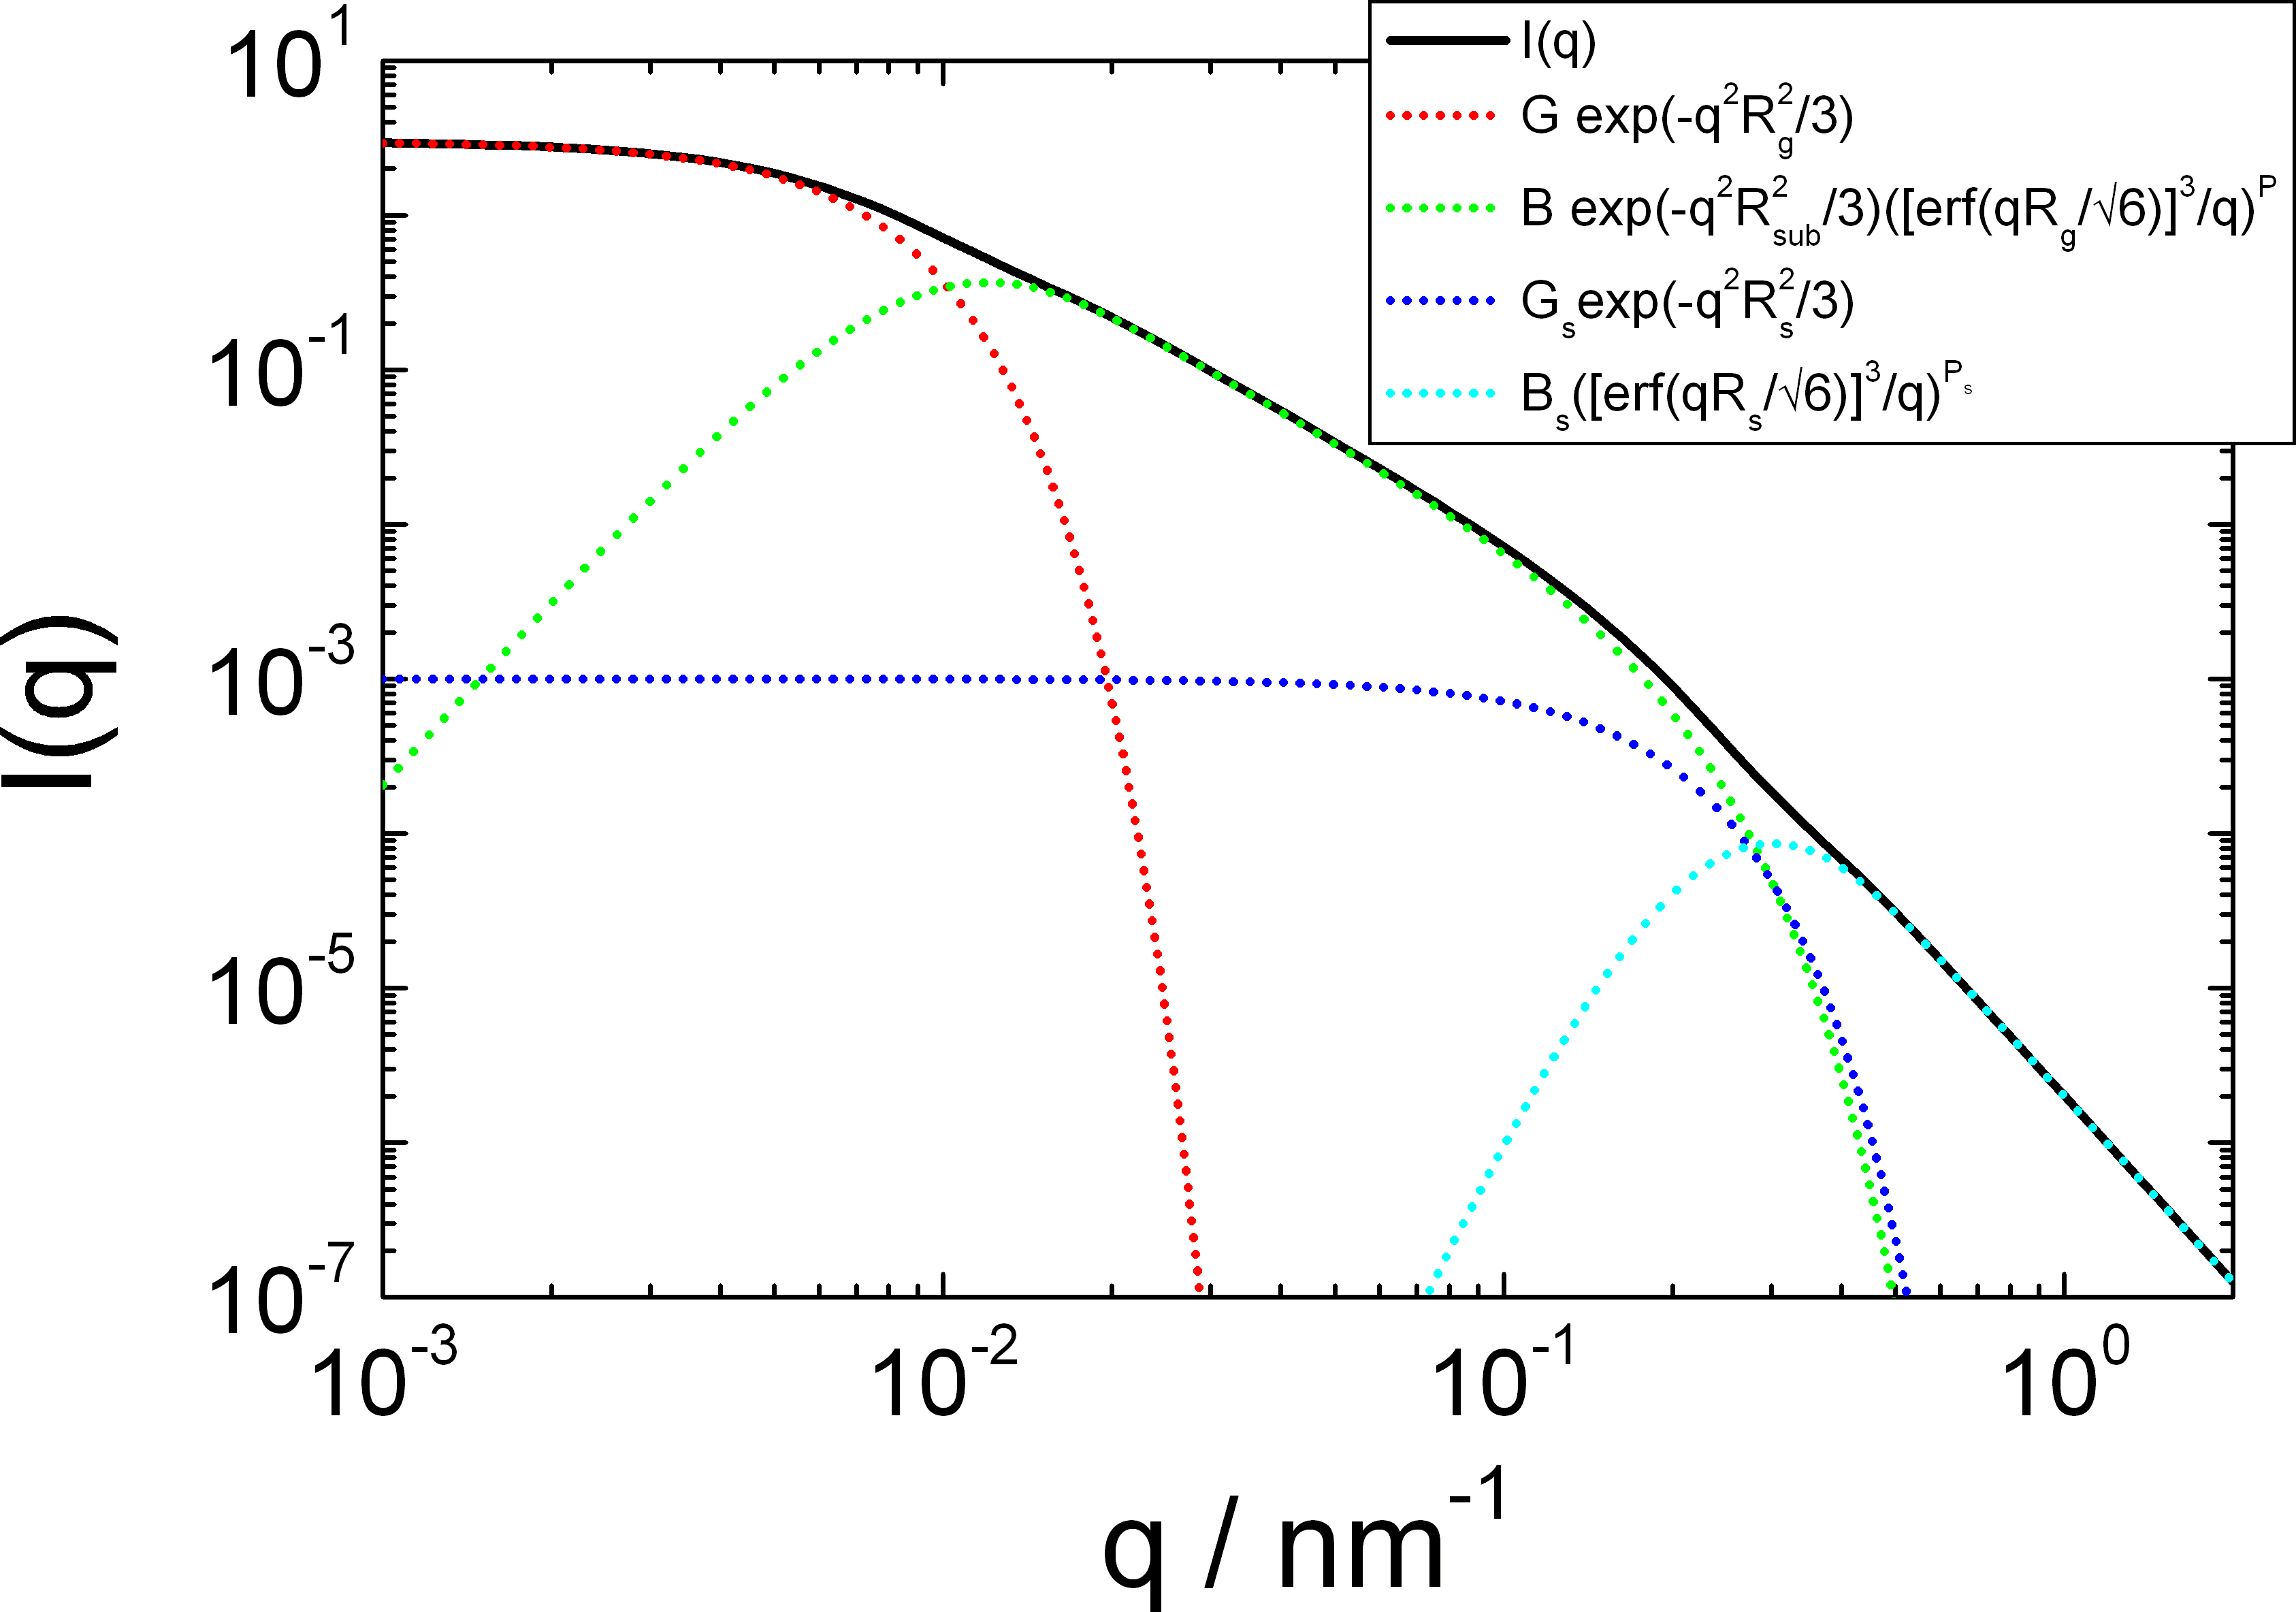
\includegraphics[width=0.75\textwidth,height=0.5\textwidth]{../images/form_factor/nonparticular/Beaucage.png}
\end{center}
\caption{}
\label{fig:Beaucage}
\end{figure}

\clearpage
\subsubsection{Beaucage2} ~\\

Equation \ref{eq:UEPL} can be extended to describe an arbitrary
number of interrelated structural levels under the
generally applicable assumption that $R_\text{sub} = R_s$,
\begin{align}
\begin{split}
I_\text{Beaucage}(Q)  \simeq \sum_{i=1}^n & G_i \exp\left(-\frac{Q^2R_{g,i}^2}{3}\right) \\
 + & B_i \exp\left(-\frac{Q^2R_{g,i+1}^2}{3}\right)
      \left( \frac{\left[\mathrm{erf}\left(Qk_iR_{g,i}/\sqrt{6}\right)\right]^3}{Q}\right)^{P_i}
\end{split}
\label{eq:generalizedUEPL}
\end{align}
In \ref{eq:generalizedUEPL}, $i= 1$ refers to the largest-size structural level.
Extensions, such as eq.\ \ref{eq:generalizedUEPL}, can only be justified when data
extend over many decades in $Q$. Eq.\ \ref{eq:generalizedUEPL} introduces no
new parameters over local Guinier and power-law fits.


\hspace{1pt}\\
\underline{Input Parameters for model \texttt{Beaucage2}:}\\
\begin{description}
\item[\texttt{G\_i}] $G_i$ is the Guinier pre-factor
\item[\texttt{B\_i}] $B_i$ is a pre-factor specific to the type of power-law scattering:
$B_i$ is defined according to the regime in which the exponent $P_i$ falls.
\item[\texttt{Rg\_i}] large-scale structure $R_{g,i}$
\item[\texttt{Rg\_i+1}] size $R_{g,i+1}$ of smaller subunits
\item[\texttt{k\_i}] This is an empirical constant that has a value of 1 for steep power-law decays,
$P > 3$. For weak power-law decays, $k$ deviates slightly from 1
\item[\texttt{k\_i+1}] This is an empirical constant that has a value of 1 for steep power-law decays,
$P_s > 3$. For weak power-law decays, $k_s$ deviates slightly from 1
\item[\texttt{P\_i}] scaling exponent of the power law assigned to the larger structure $R_{g,i}$
\item[\texttt{P\_i+1}] scaling exponent of the power law assigned to the smaller structure $R_{g,i+1}$
\end{description}

\begin{figure}[htb]
\begin{center}
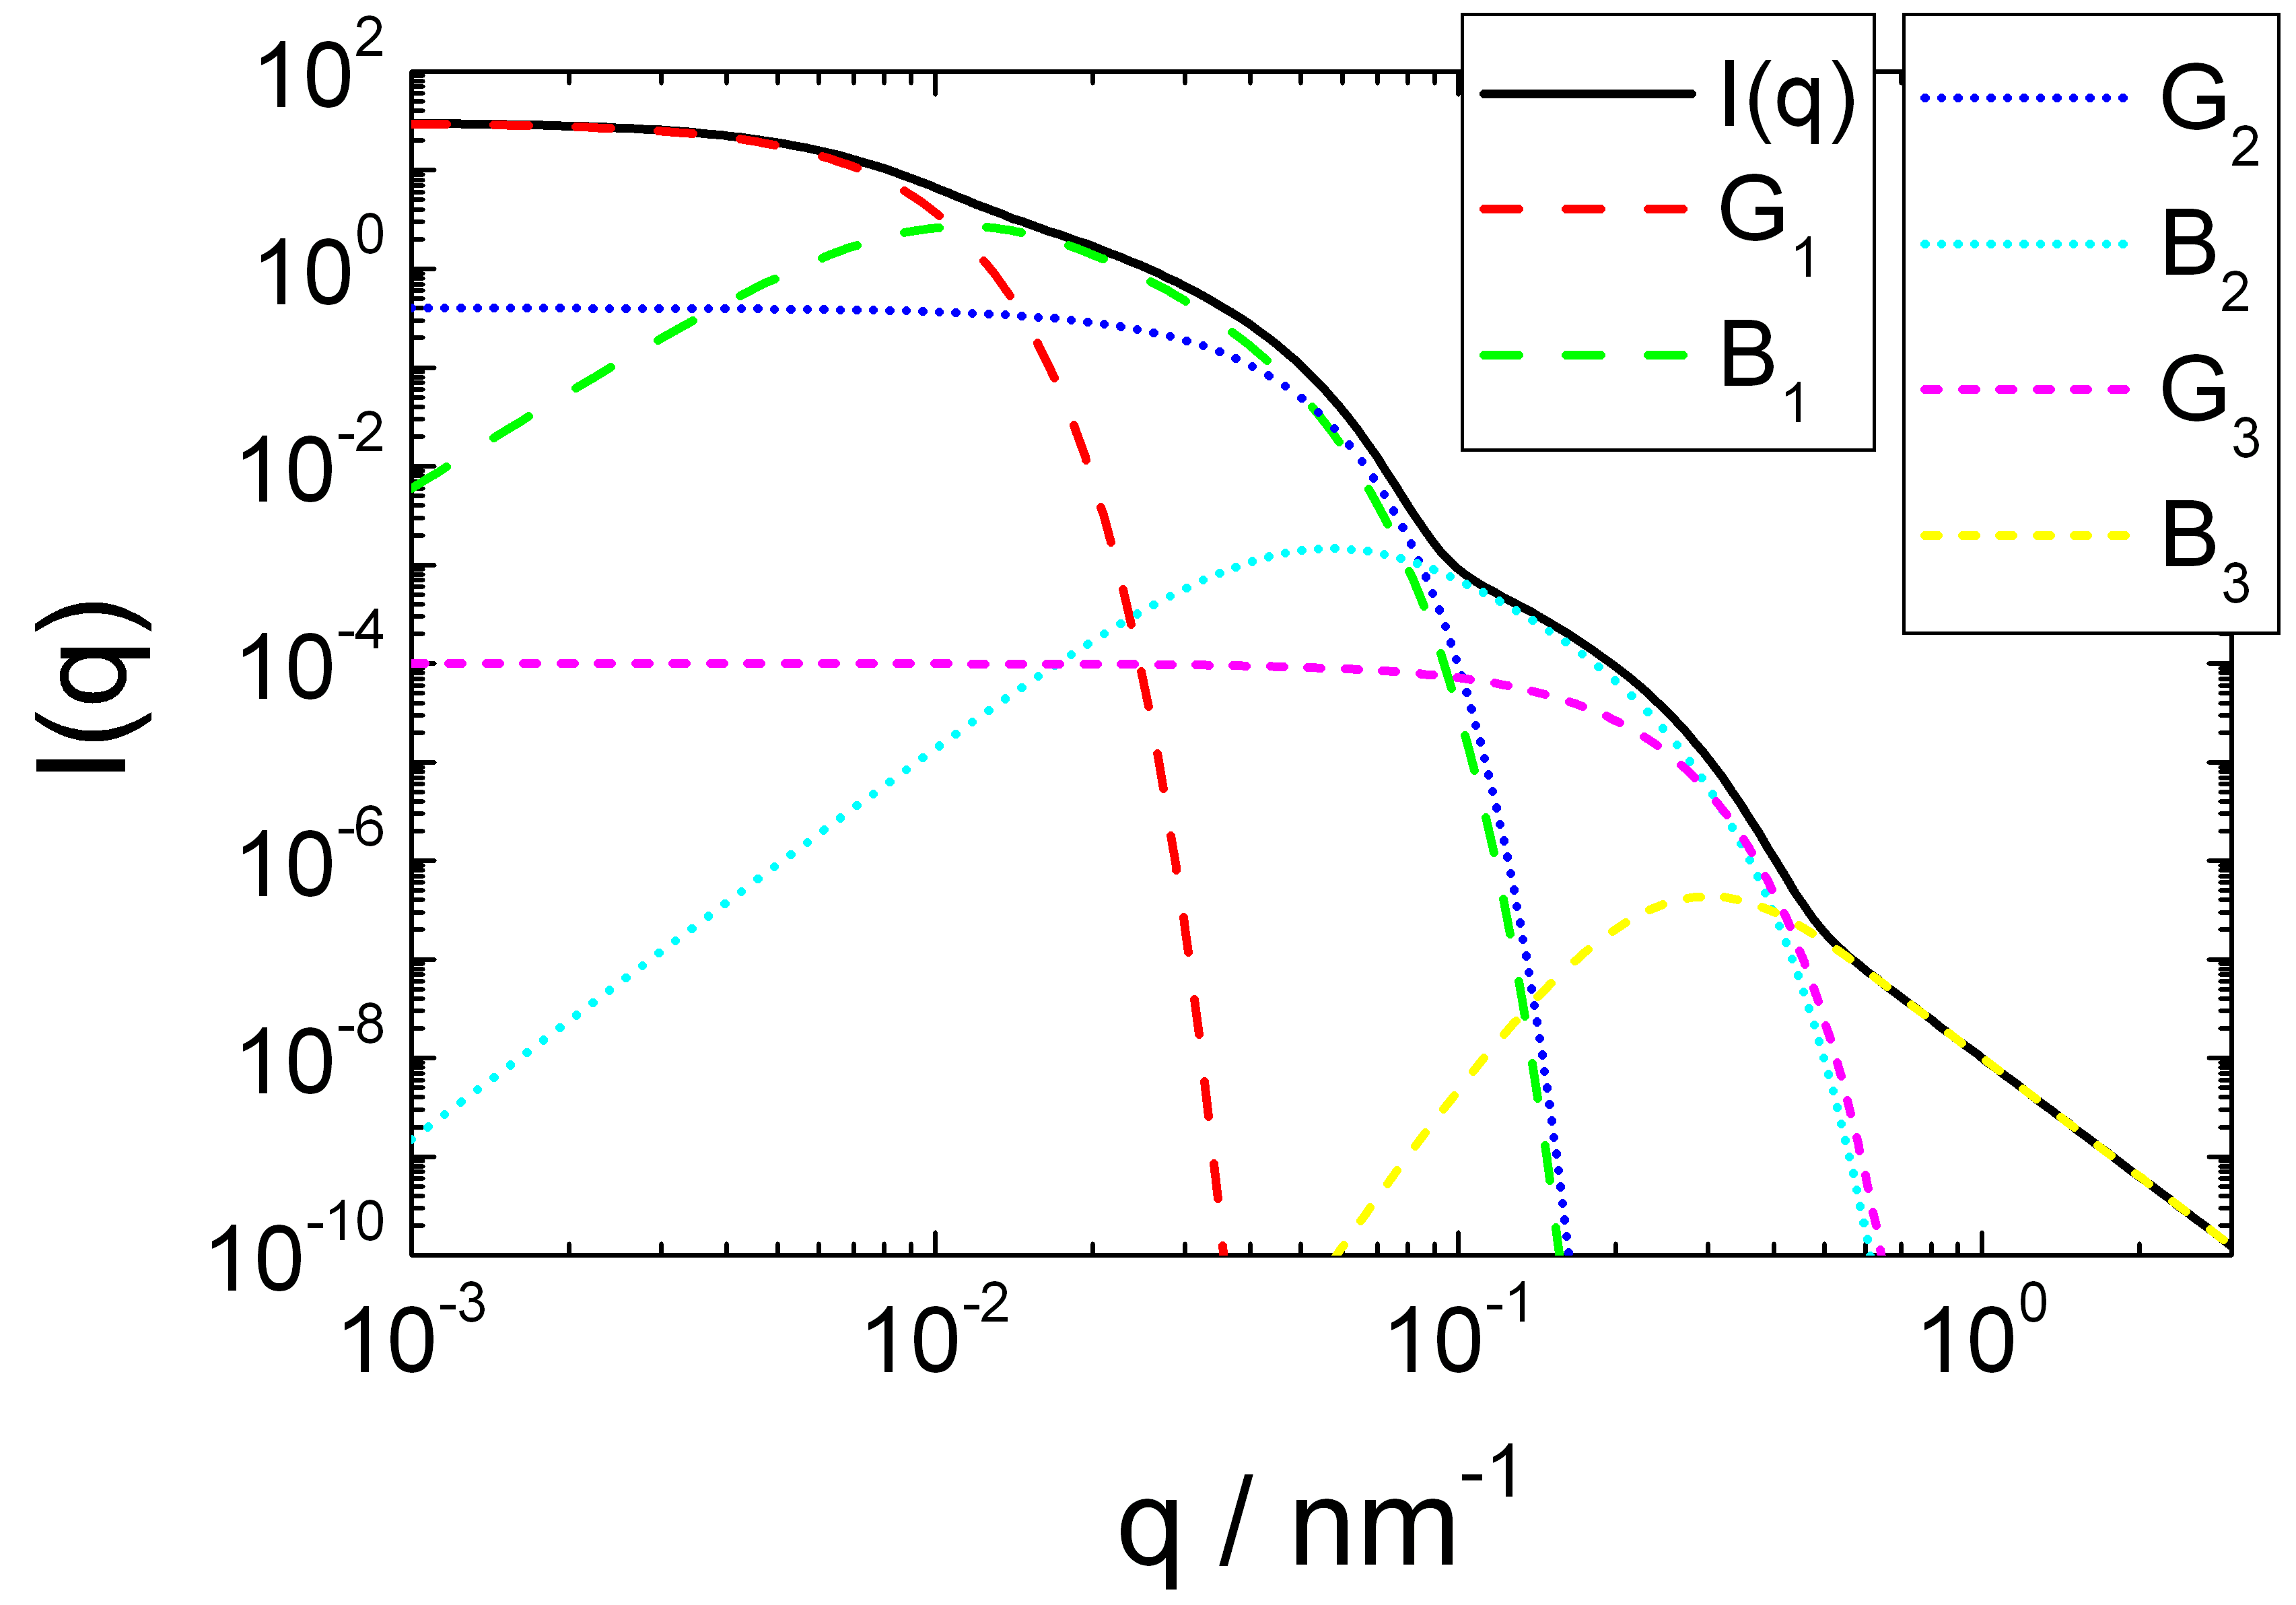
\includegraphics[width=0.75\textwidth,height=0.5\textwidth]{../images/form_factor/nonparticular/Beaucage2.png}
\end{center}
\caption{}
\label{fig:Beaucage2}
\end{figure}

%\noindent REFERENCE:\\
%G. Beaucage, Approximations Leading to a Unified
%Exponential/Power-Law Approach to Small-Angle Scattering, J. Appl.
%Cryst. (1995). 28, 717-728 \\
%G. Beaucage, Small-Angle Scattering from Polymeric Mass Fractals
%of Arbitrary Mass-Fractal Dimension,  J. Appl. Crystallogr. , 29,
%134-146 (1996).

%%%%%%%%%%%%%%%%%%%%%%%%%%%%%%%%%%%%%%%%%%%%%%%%%%%%%%%%%%%%%%%%%%%%%%%%%

\clearpage
\subsection{WormLikeChainEXV \cite{Pedersen96Macrom}}
\label{sect:WormLikeChain}
~\\
\begin{figure}[htb]
\begin{center}
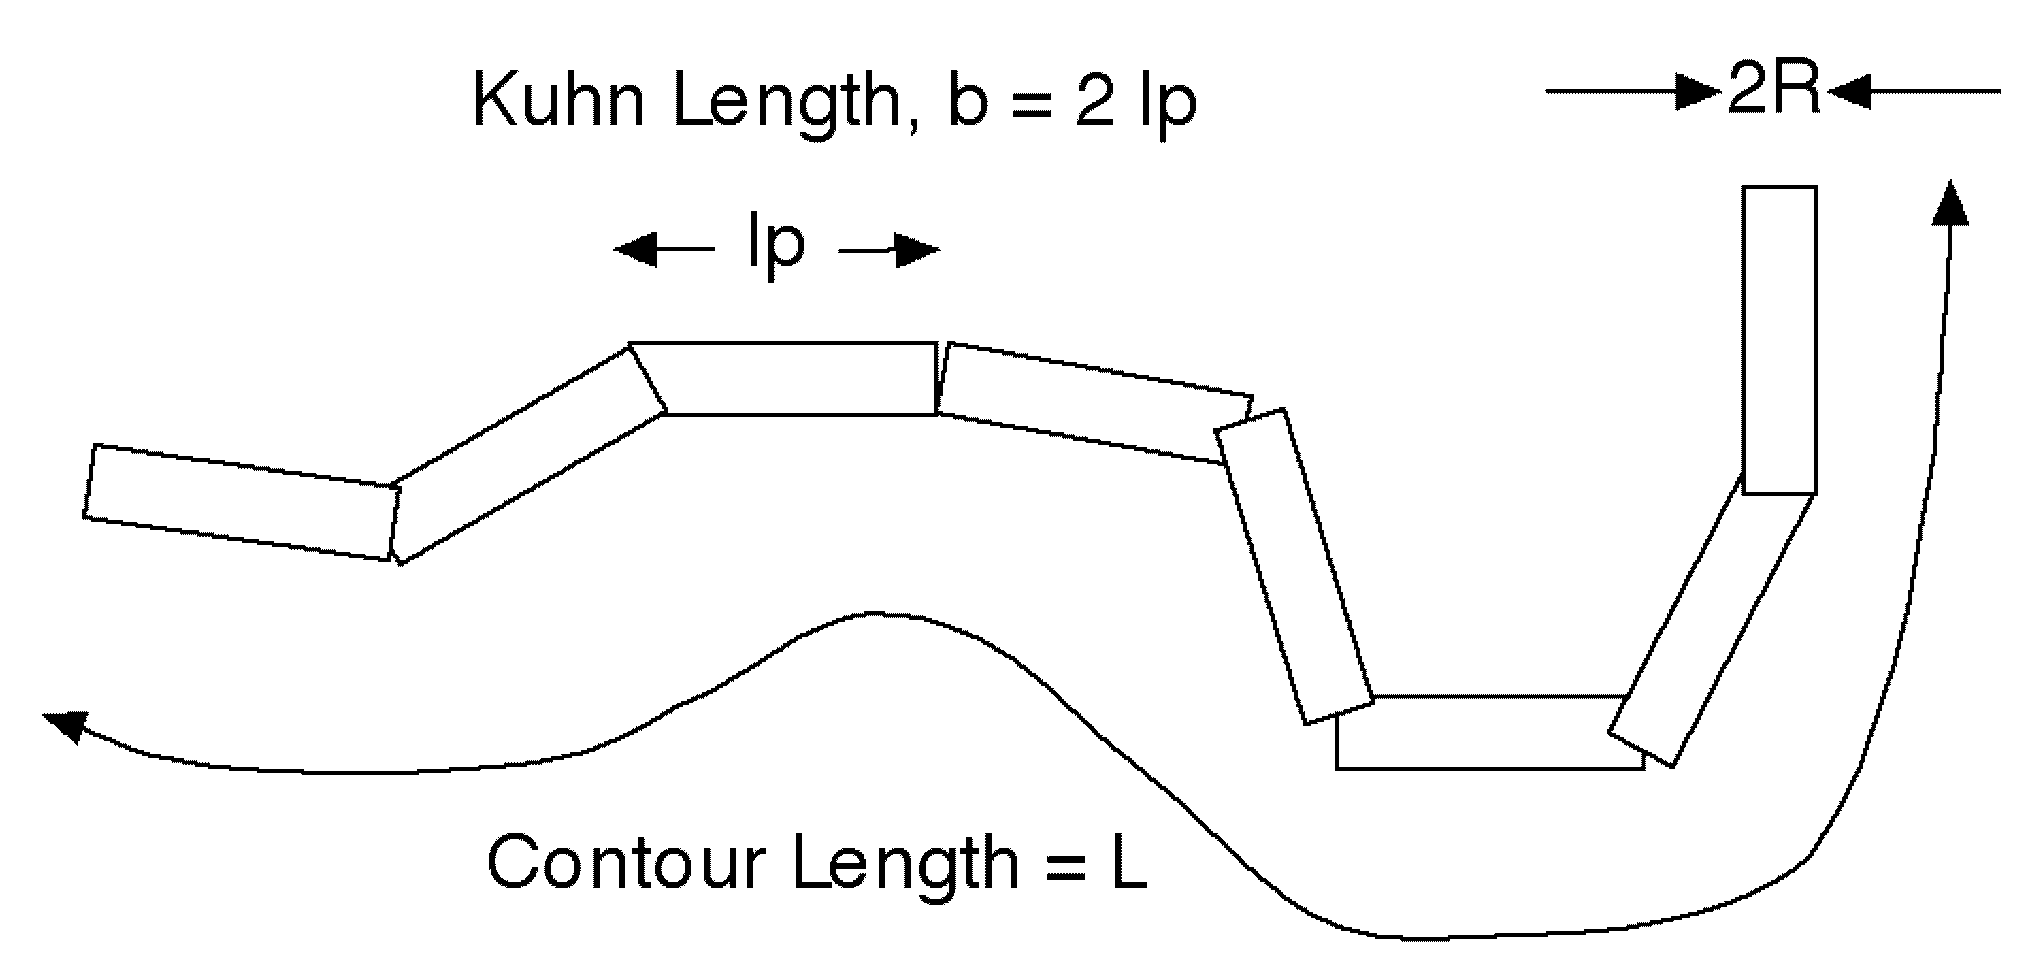
\includegraphics[width=0.8\textwidth,height=0.4\textwidth]{wormlike2.png}
\end{center}
\caption{The chain of contour length, $L$, (the total length) can
be described a chain of some number of locally stiff segments of
length $l_p$. The persistence length,$l_p$, is the length along
the cylinder over which the flexible cylinder can be considered a
rigid rod. The Kuhn length ($b$) used in the model is also used to
describe the stiffness of a chain, and is simply $b = 2l_p$.}
\label{wormlike2}
\end{figure}

This form factor calculates the form factor for a flexible
cylinder with a circular cross section and a uniform scattering
length density. The non-negligible diameter of the cylinder is
included by accounting for excluded volume interactions within the
walk of a single cylinder. Inter-cylinder interactions are NOT
included. The function calculated has been given by Pedersen et al.\
\cite{Pedersen96Macrom}. The model "Method 3 With Excluded Volume" is used,
which is a parametrization of simulations of a discrete
representation of the worm-like chain model of Kratky and Porod
applied in the pseudo-continuous limit.

\vspace{5mm}

\hspace{1pt}\\
\underline{Input Parameters for model \texttt{WormLikeChainEXV}:}\\
\begin{description}
\item[\texttt{R}] radius $R$ of cylindrical core with uniform scattering length density
\item[\texttt{l}] Kuhn length\footnote{The Kuhn length $l$ is related to the length $a$ of
    locally stiff segment simply via $l=2a$} $l$ of semi-flexible worm-like structure
\item[\texttt{L}] contour length $L$ of semi-flexible worm-like structure
\end{description}

\begin{figure}[htb]
\begin{center}
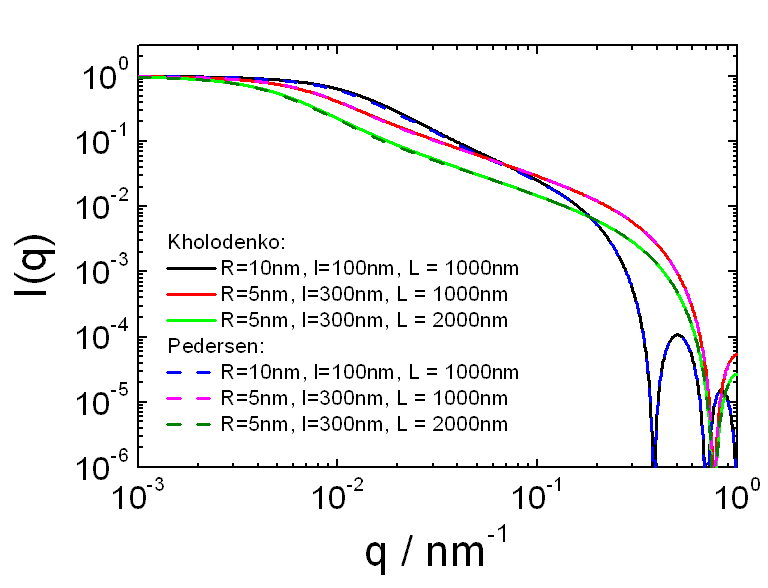
\includegraphics[width=0.768\textwidth,height=0.588\textwidth]{wormlike_Iq.png}
\end{center}
\caption{Comparison of wormlike micelles according to Pedersen \cite{Pedersen96Macrom}
and Kholodenko \cite{kholodenko93}} \label{fig:wormlike_Iq}
\end{figure}


%%%%%%%%%%%%%%%%%%%%%%%%%%%%%%%%%%%%%%%%%%%%%%%%%%%%%%%%%%%%%%%%%%%%%%%%%

\clearpage
\subsection{KholodenkoWorm}
\label{sect:KholodenkoWorm}~\\

\begin{figure}[htb]
\begin{center}
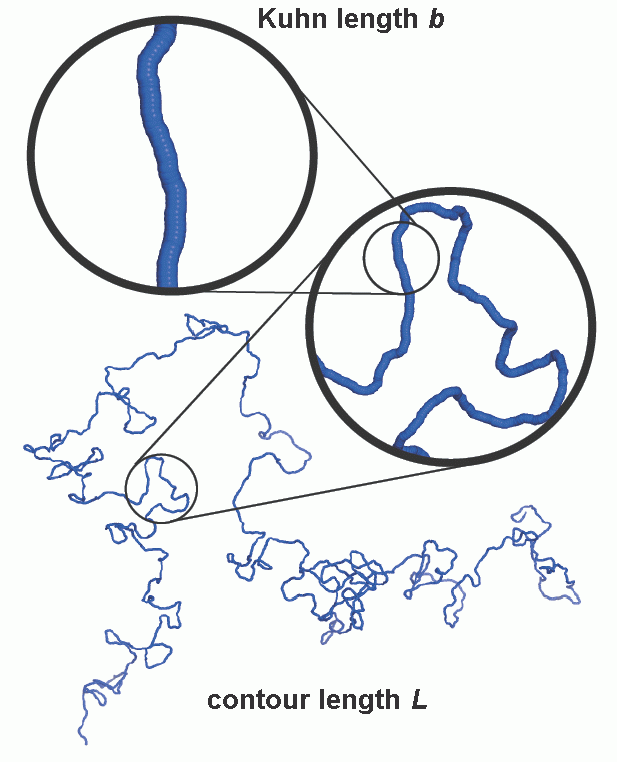
\includegraphics[width=0.617\textwidth,height=0.762\textwidth]{SemiflexiblePolymerTxt.png}
\end{center}
\caption{}
\label{fig:KholodenkoWorm}
\end{figure}

Kholodenko \cite{kholodenko93} presented a new approach using the analogy between Dirac�s fermions
and semi-flexible polymers. The form factor $P_0(Q)$ resulting
from Kholodenko�s approach is designed to reproduce
correctly the rigid-rod limit and the random-coil limit.
Defining $x = 3L/l$ ($L$: contour length, $l$: Kuhn length), it is given by
\begin{align}
P_0(Q,L,l) &= \frac{2}{x} \left[I_{(1)} -\frac{1}{x}I_{(2)}\right]
\label{eq:Kholodenko}
\end{align}
where
\begin{align}
I_{(n)}(x) &= \int_0^x  f(z) \, z^{n-1} \, dz
\end{align}
together with
\begin{align}
f(z)) &=
\begin{cases} \displaystyle
\frac{1}{E}\frac{\sinh(Ez)}{\sinh(z)} & \text{for} \quad \displaystyle Q \leq \frac{3}{l}\\ \\
\displaystyle
\frac{1}{F}\frac{\sin(Fz)}{\sinh(z)} & \text{for} \quad \displaystyle Q > \frac{3}{l}
\end{cases}
\end{align}
and
\begin{align}
E = \sqrt{1-\left(\frac{lQ}{3}\right)^2} \quad \text{and} \quad F = \sqrt{\left(\frac{lQ}{3}\right)^2-1}
\end{align}

For flexible cylinders with a circular cross section and a uniform scattering
length density the cross section form factor is given by
\begin{align}
P_{cs} = \left(2 \frac{J_1(QR)}{QR}\right)^2
\end{align}
so that the overall form factor is given by
\begin{align}
P(Q,L,l,R) = P_0(Q,L,l)\, P_{cs}(Q,R)
\end{align}

\vspace{5mm}

\hspace{1pt}\\
\underline{Input Parameters for model \texttt{KholodenkoWorm}:}\\
\begin{description}
\item[\texttt{R}] radius $R$ of cylindrical core with uniform scattering length density
\item[\texttt{l}] Kuhn length\footnote{The Kuhn length $l$ is related to the length $a$ of
    locally stiff segment simply via $l=2a$} $l$ of semi-flexible worm-like structure
\item[\texttt{L}] contour length $L$ of semi-flexible worm-like structure
\end{description}

\begin{figure}[htb]
\begin{center}
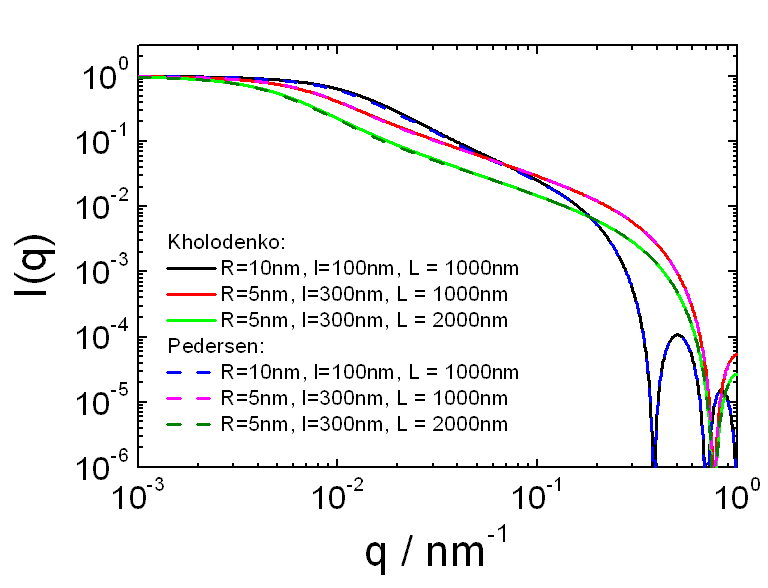
\includegraphics[width=0.768\textwidth,height=0.588\textwidth]{wormlike_Iq.png}
\end{center}
\caption{Comparison of wormlike micelles according to Pedersen \cite{Pedersen96Macrom}
and Kholodenko \cite{kholodenko93}. } \label{fig:wormlike_Iq2}
\end{figure}

%%%%%%%%%%%%%%%%%%%%%%%%%%%%%%%%%%%%%%%%%%%%%%%%%%%%%%%%%%%%%%%%%%%%%%%%%
\clearpage

\subsection{Diblock copolymer micelles}
\label{subsect:DiblockCopolymerMicelles}
~\\
\begin{figure}[htb]
\centering
  \subfigure[spherical
  micelle]{\quad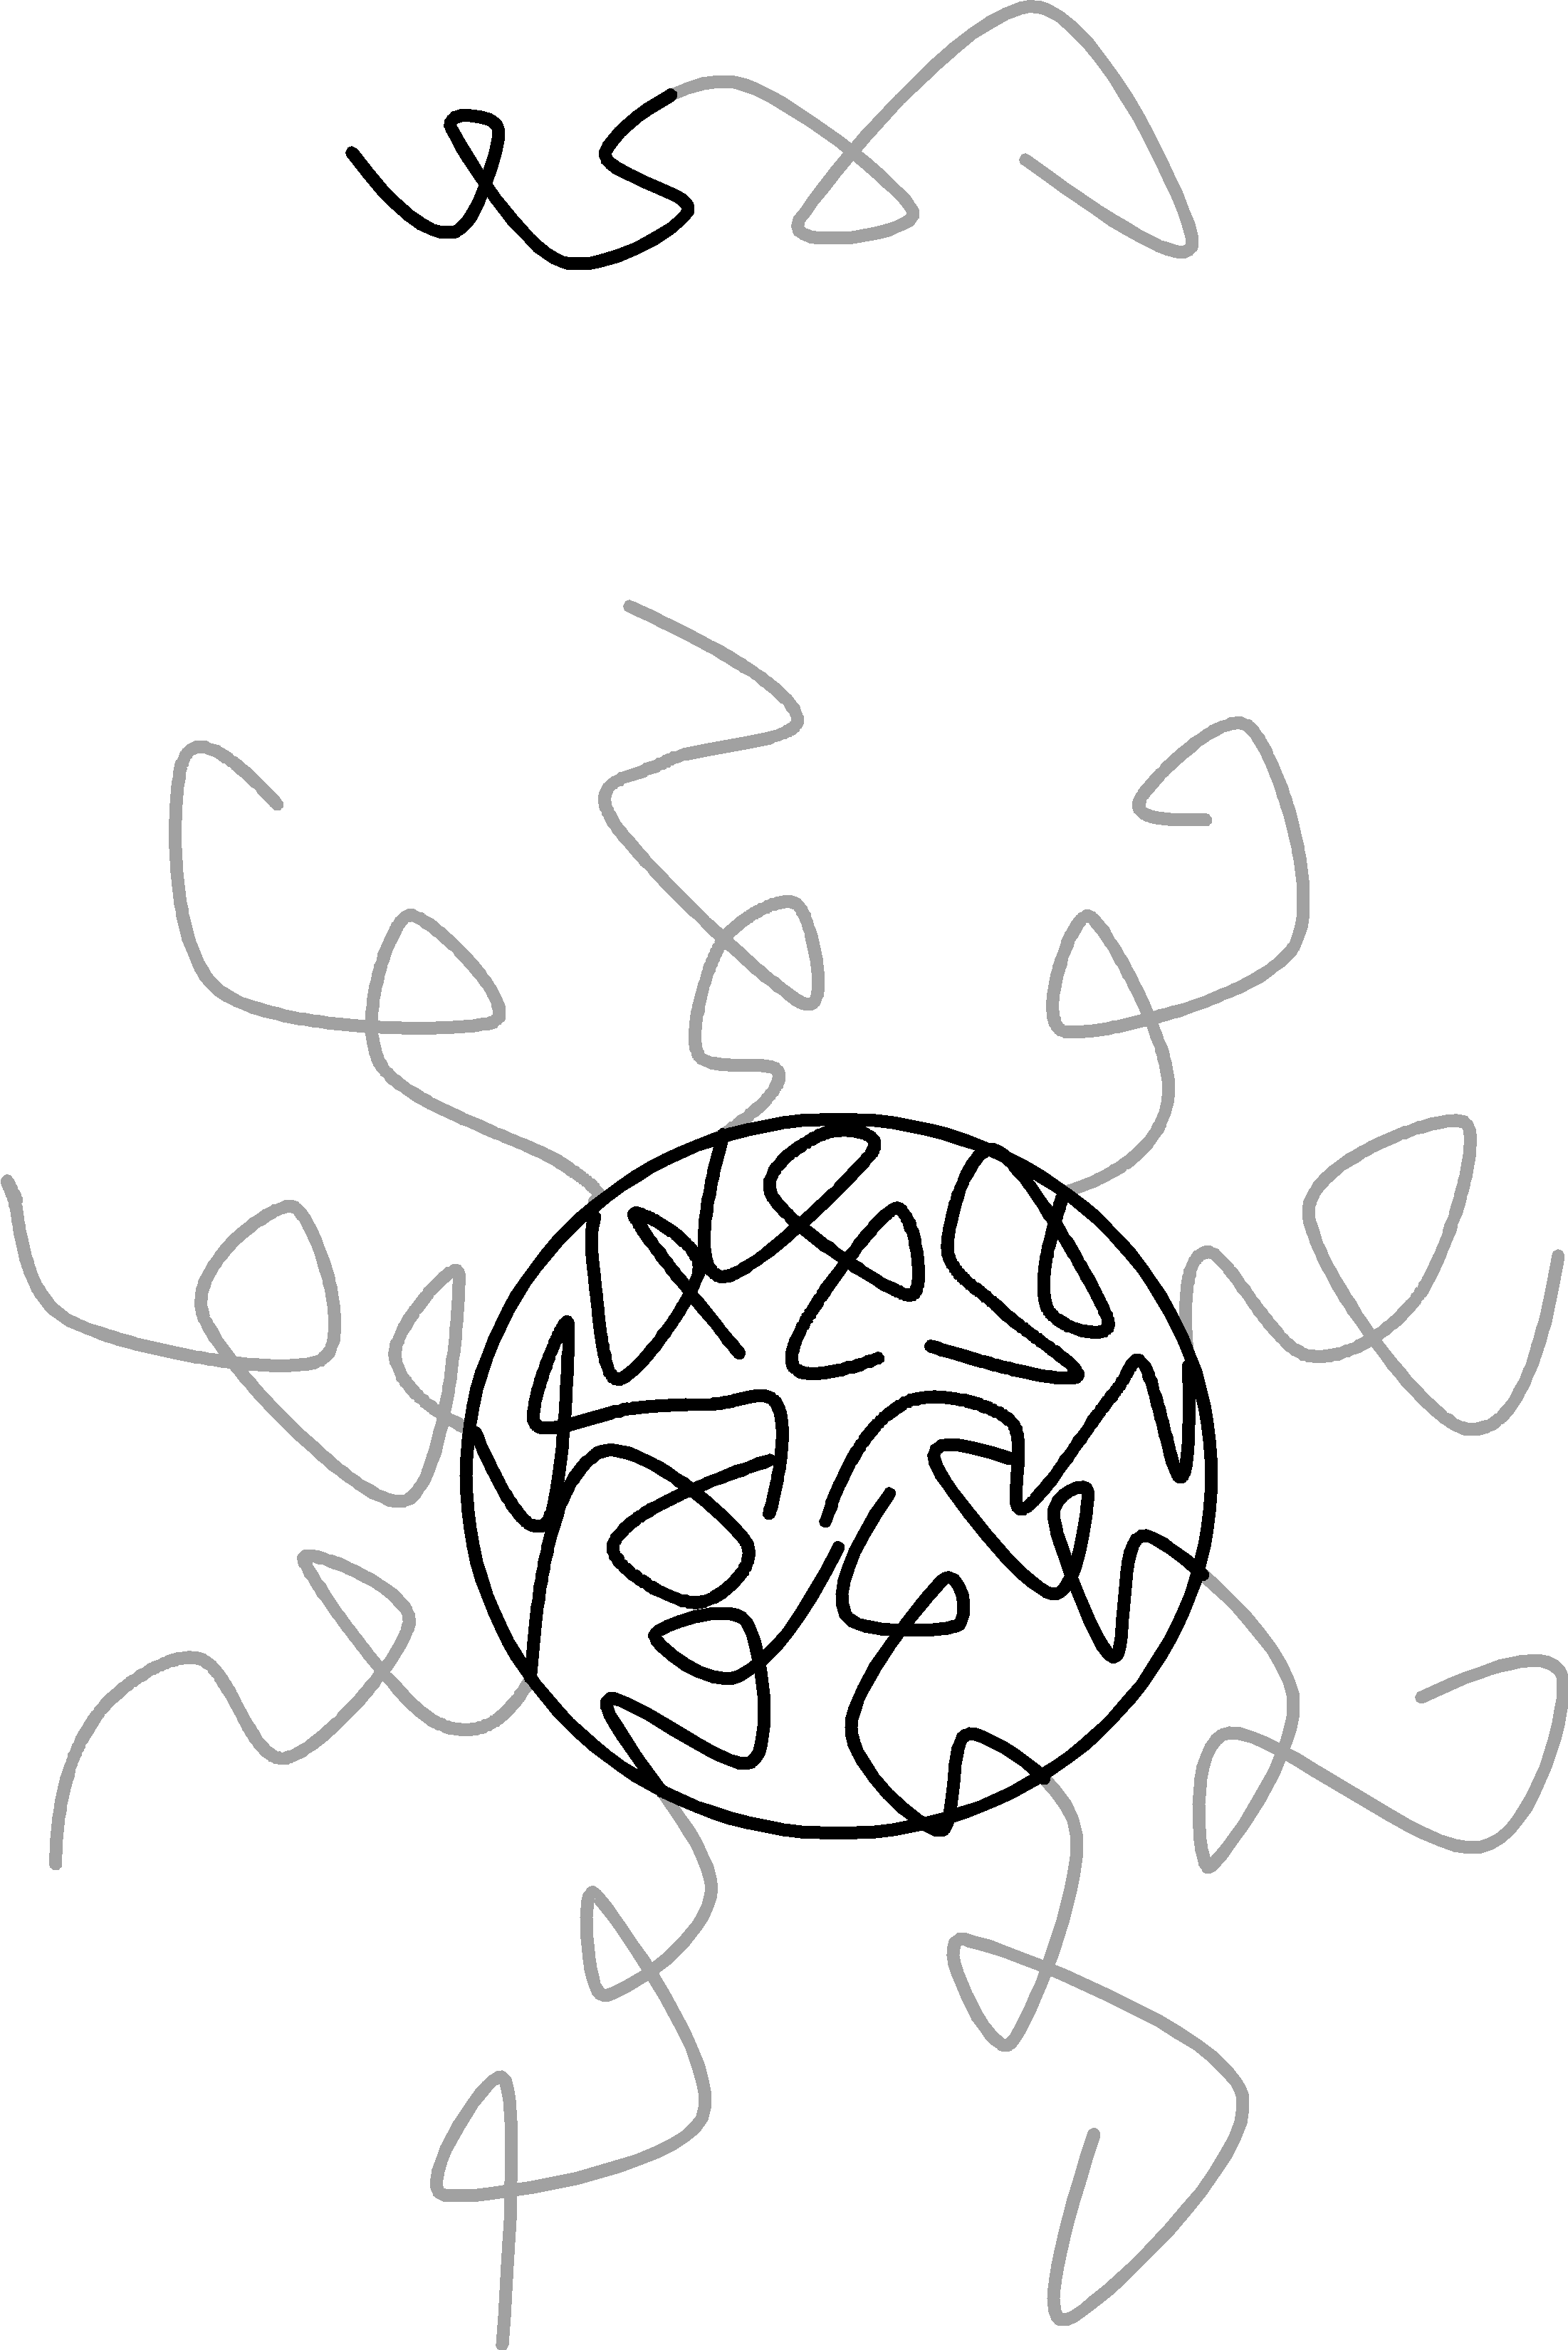
\includegraphics[width=0.25\textwidth,height=0.375\textwidth]{spheregauss.png}\quad}
  \quad
  \subfigure[ellipsoidal
  micelle]{\quad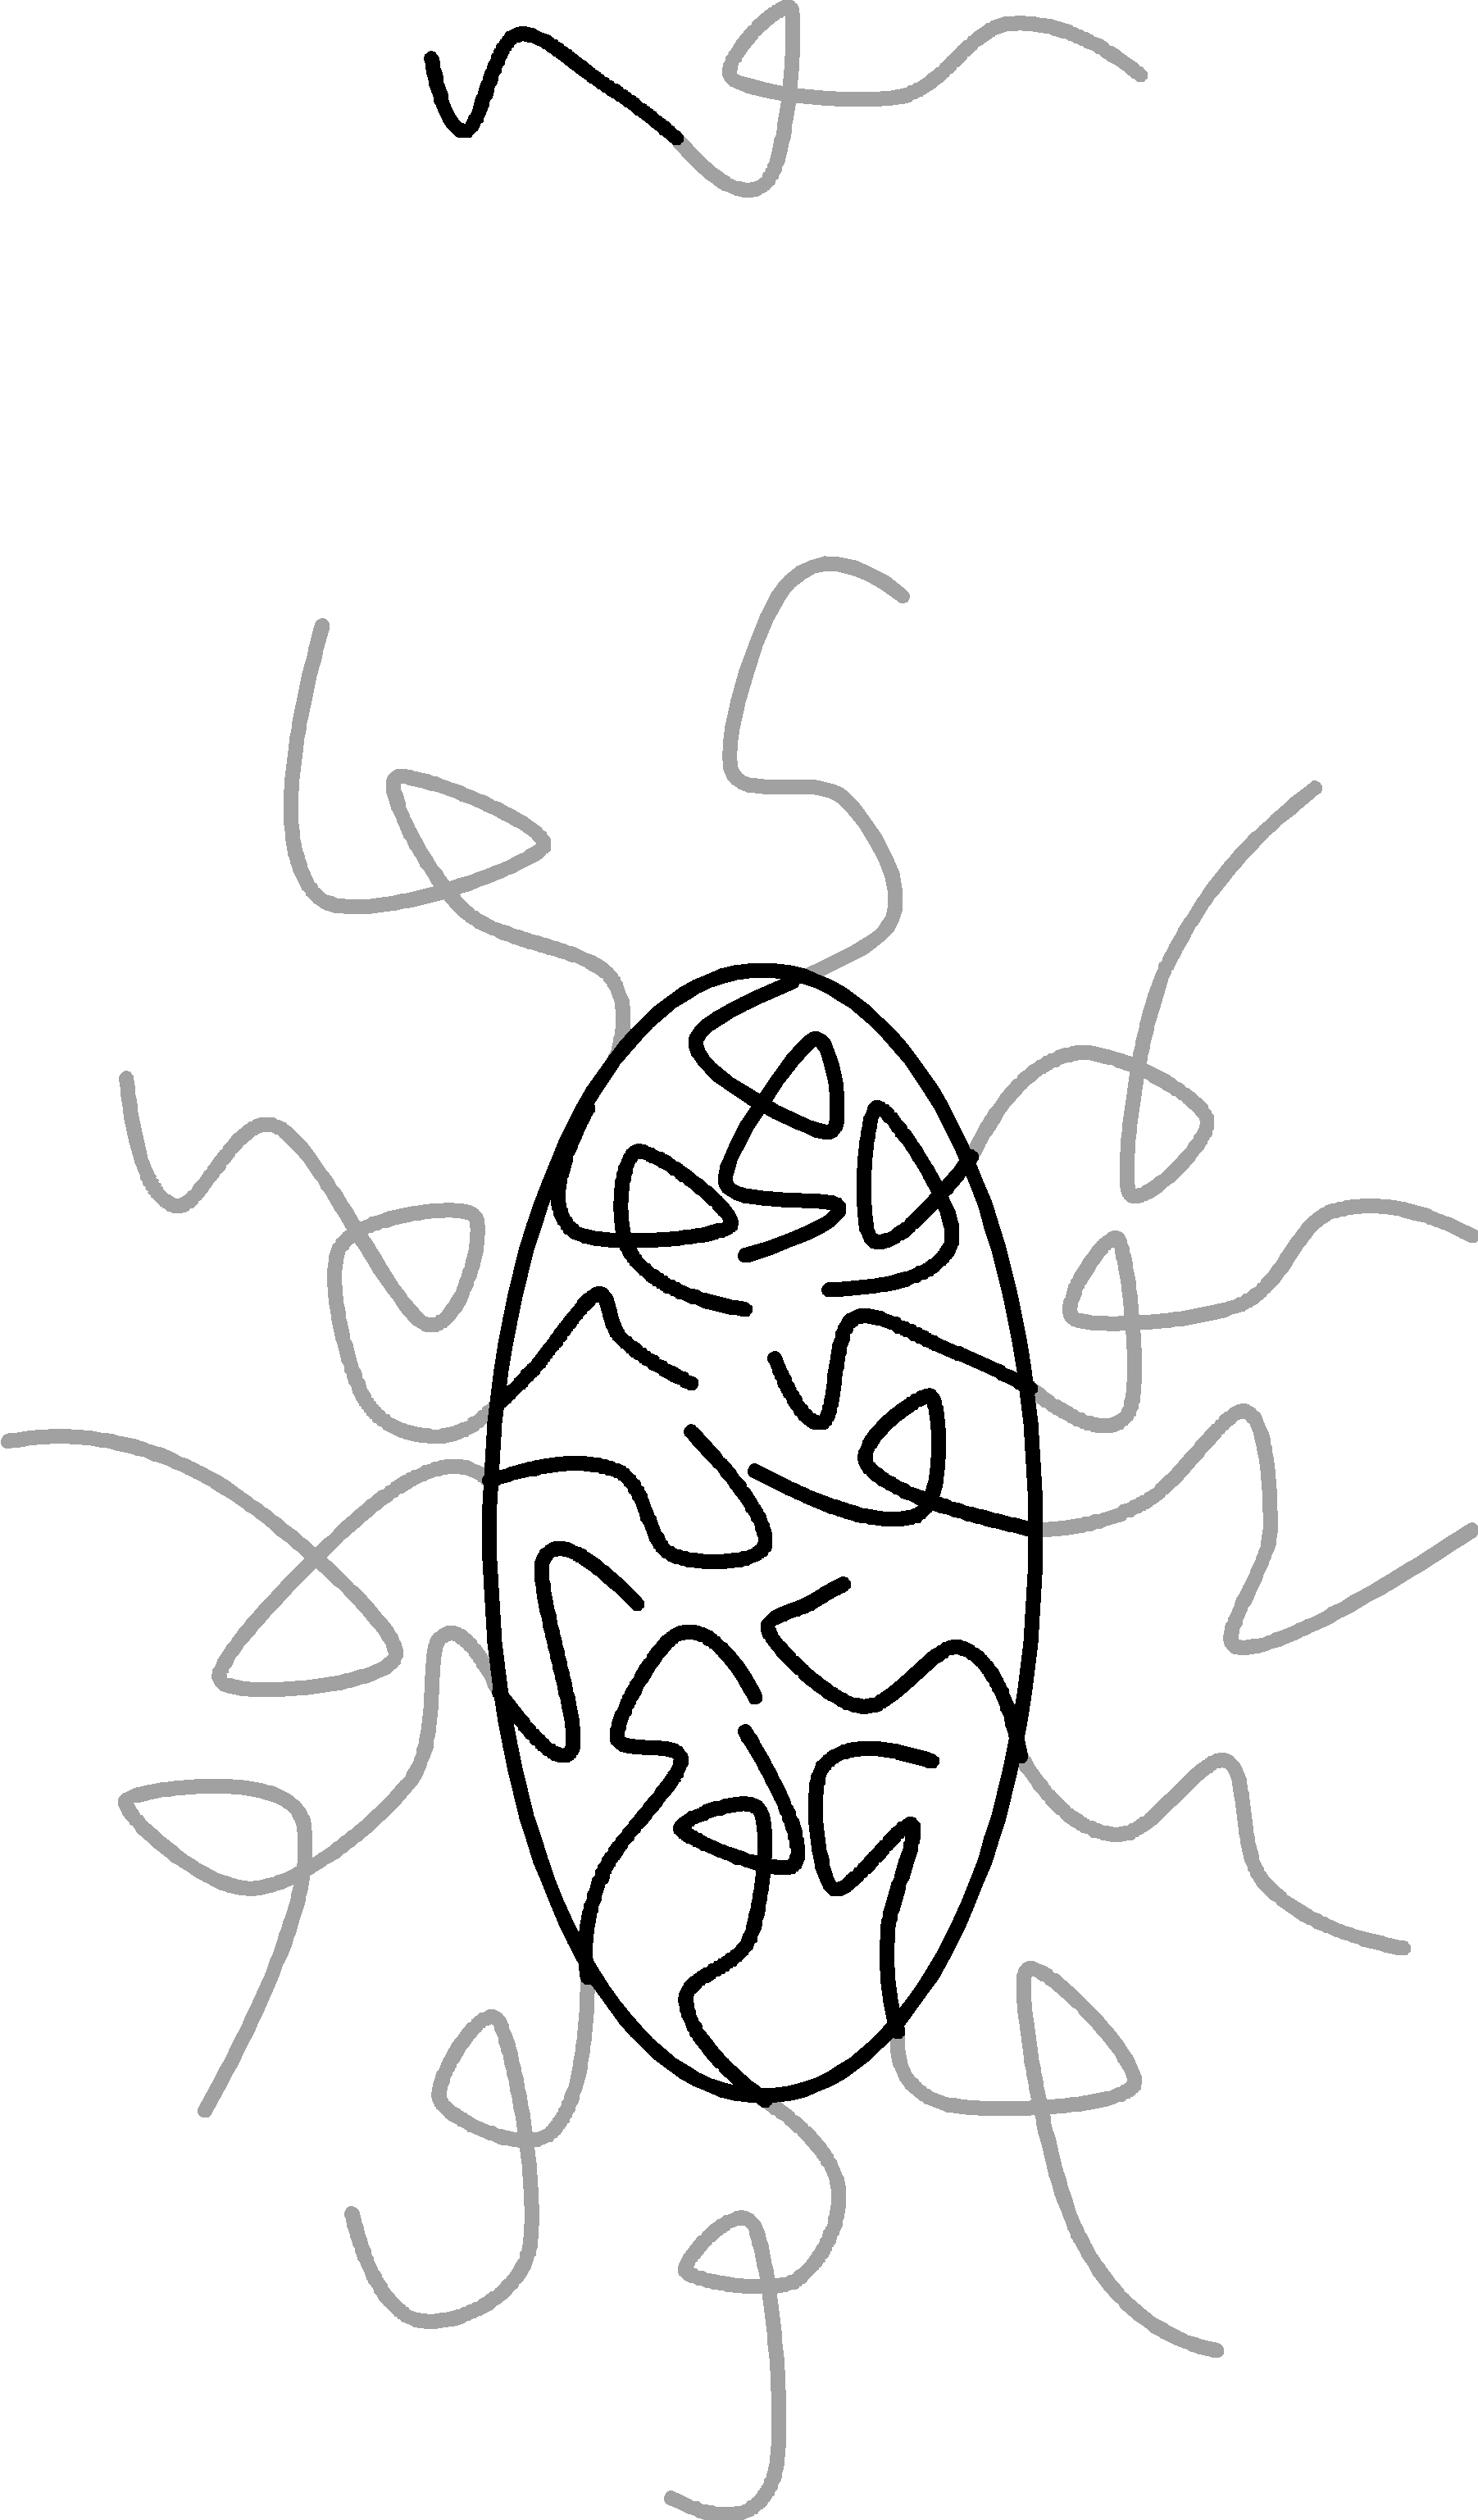
\includegraphics[width=0.25\textwidth,height=0.41\textwidth]{ellipsoidgauss.png}\quad}
  \quad
  \subfigure[cylindrical micelle]{\quad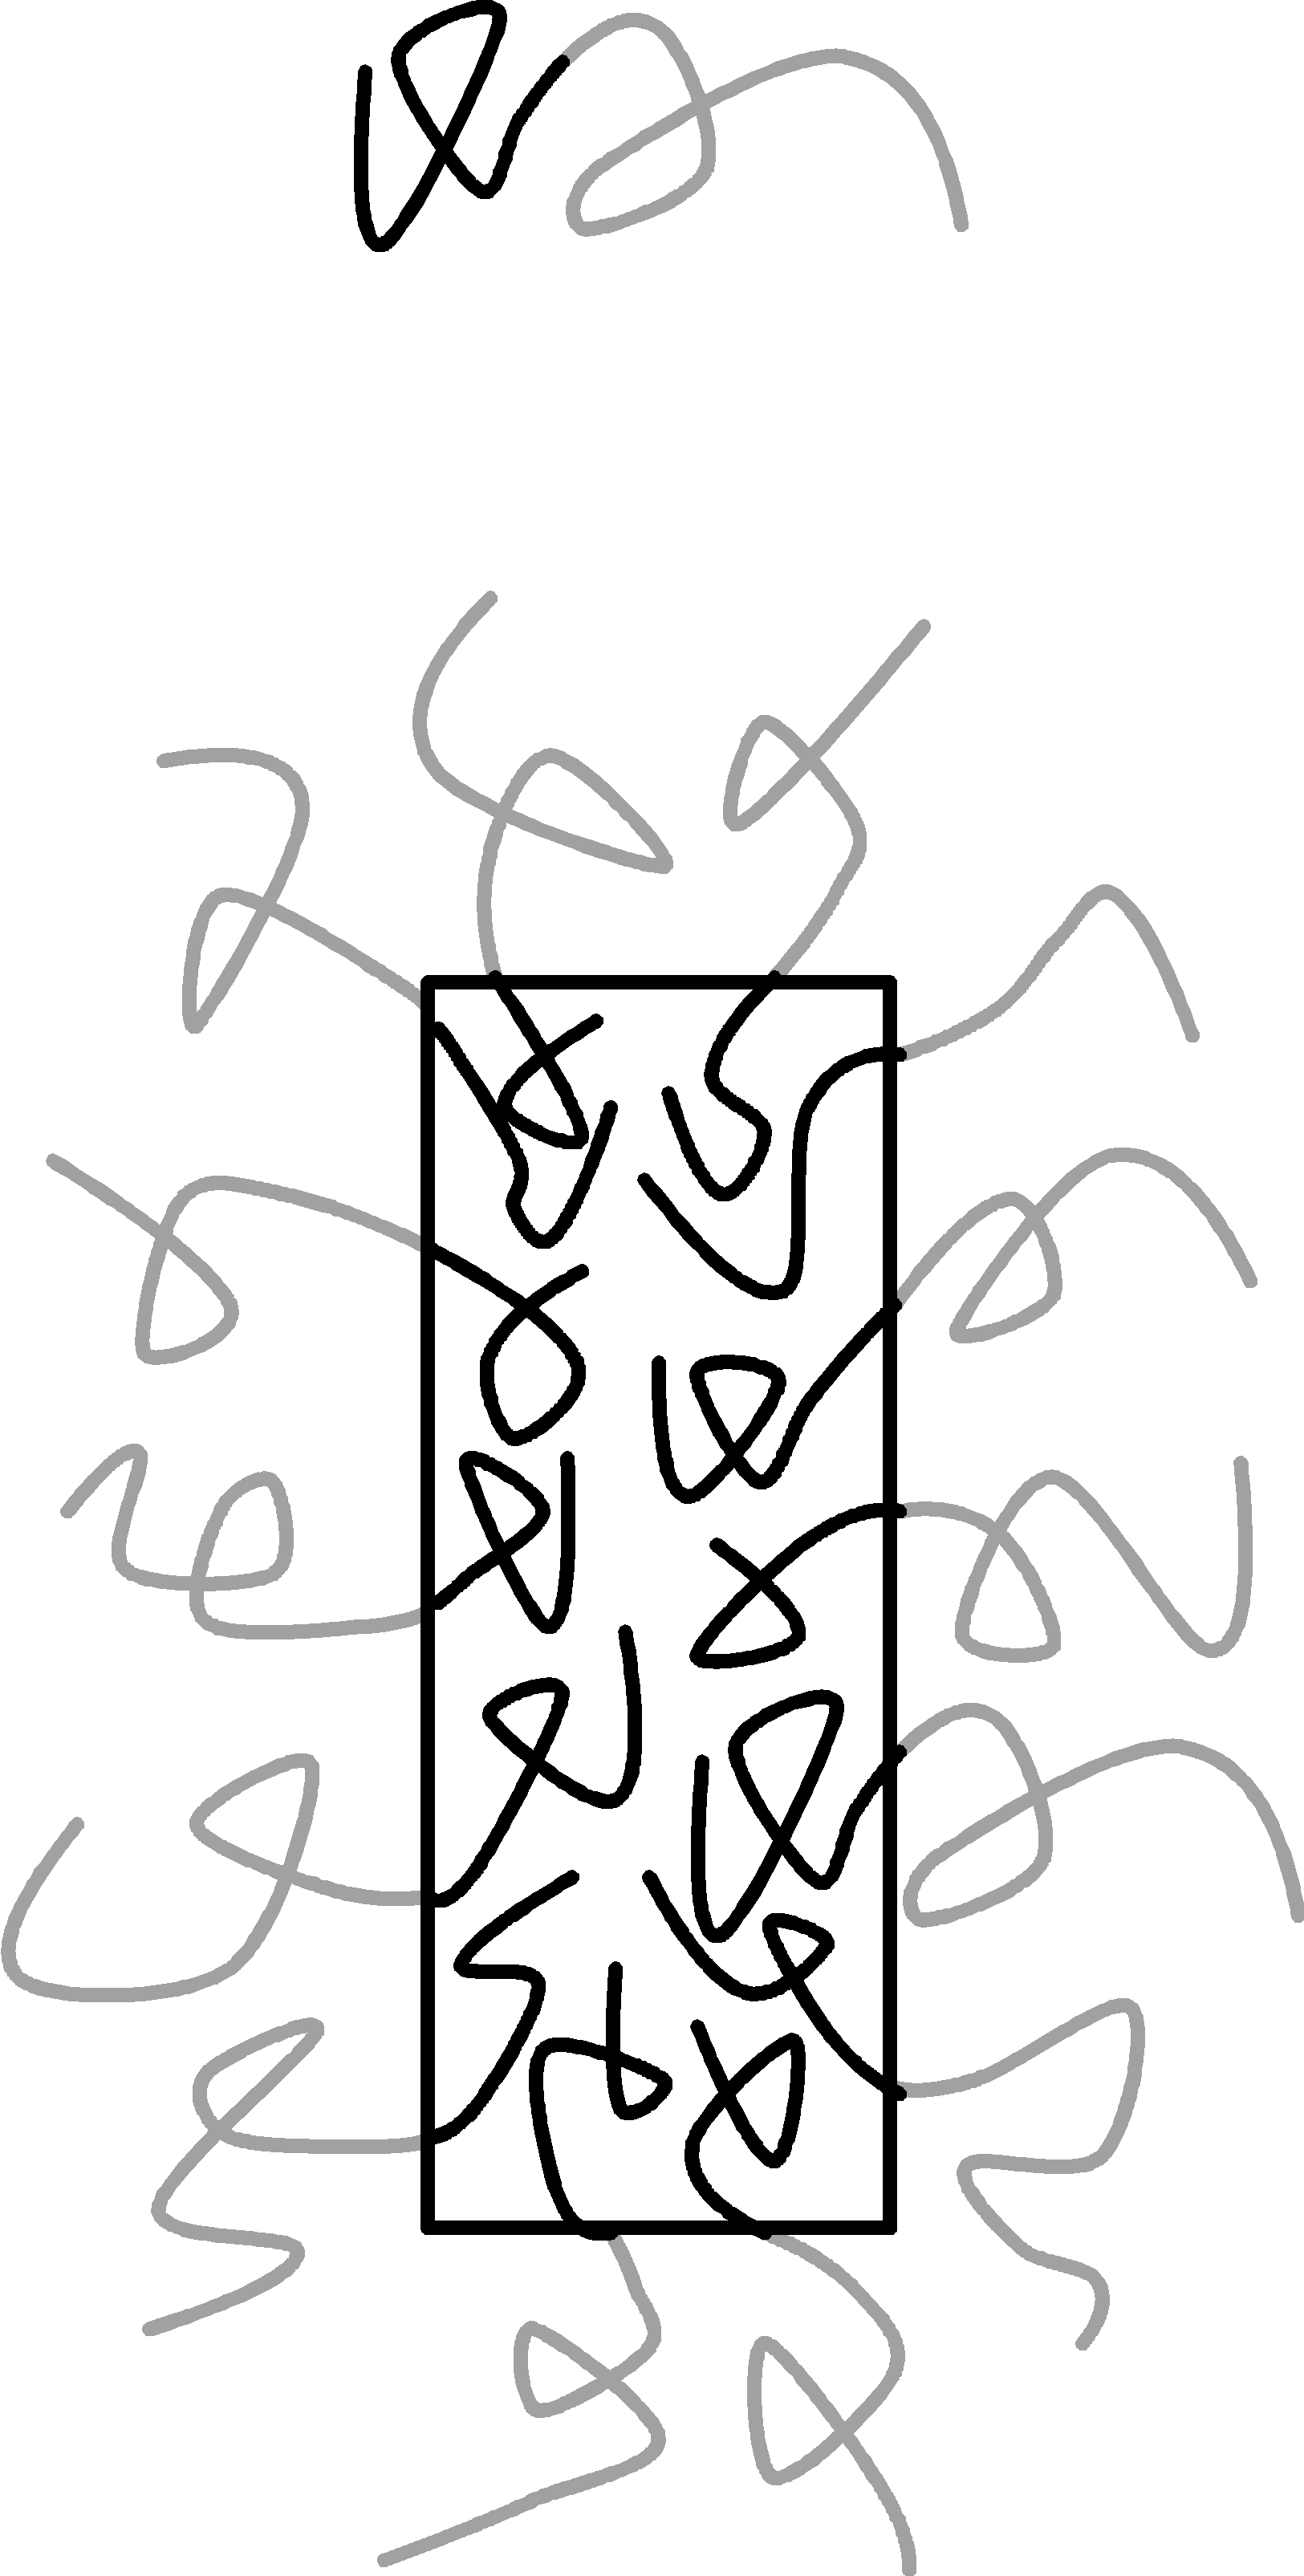
\includegraphics[width=0.2\textwidth,height=0.4\textwidth]{cylindergauss.png}\quad}
  \caption{Block copolymer forming micelles of different shapes}
\end{figure}

For block copolymers, which form micelles, several form factor have
been implemented \cite{PedersenGerstenberg96,PedersenJApplCryst2000,SvaneborgPedersen2002}
for spherical, ellipsoidal, and cylindrical shapes.
It has been assumed that one unit is forming the core of the
micelles and the other the corona. The core is assumed to have a
homogeneous scattering length density, but may contain some amount
of solvent. For the polymer chains in the corona either a model
where Gaussian chains are attached to the core or a corona model of
semi-flexible interacting self-avoiding chains (only for spherical
core) or a continuous model, where a radial profile of the form
$\Phi(r)\varpropto r^{-\alpha}$ has been assumed. The form factors
have been parameterized such, that the excess scattering of the
corona and the core are consistent with the composition and density
of the two separate block units of the copolymer.

\vspace{3mm}
\subsubsection{Micelles with a homogeneous core and Gaussian chains on the surface}
\label{Chains(RW)} ~\\
%\phantomsection
%\addcontentsline{toc}{subsubsection}{\indexname}
%\printindex

It is assumed that the diblock copolymer consist of a block unit for
which the solvent is poor and a block unit with is good. The
insoluble blocks form a relatively compact core whereas the soluble
blocks form a diffuse corona surrounding the core. The form factor
of a micelle contains four different terms: the self-correlation
term of the core $N_\text{agg}^2\beta_\text{core}^2\,P_\text{core}(q)$,
the self-correlation term of the chains
$N_\text{agg}\beta_\text{brush}^2\,P_\text{brush}(q)$, the cross-term
between the core and chains
$2N_\text{agg}^2\beta_\text{core}\beta_\text{brush}\,S_\text{brush-core}(q)$,
and the cross term between different chains
$N_\text{agg}(N_\text{agg}-1)\beta_\text{brush}^2\,S_\text{brush-brush}(q)$.
It can be written (Pedersen \& Gerstenberg, 1996)
\begin{align}
I_\text{mic}    &= N_\text{agg}^2\beta_\text{core}^2\,P_\text{core}(q) + N_\text{agg}\beta_\text{brush}^2\,P_\text{brush}(q)  \label{eq:micelle}\\
                &+ 2N_\text{agg}^2\beta_\text{core}\beta_\text{brush}\,S_\text{brush-core}(q) + N_\text{agg}(N_\text{agg}-1)\beta_\text{brush}^2\,S_\text{brush-brush}(q)\nonumber
\end{align}
$N_\text{agg}$ is the aggregation number of diblock polymers forming
the micelle and $\beta_\text{brush}=V_\text{brush}(\eta_\text{brush}-\eta_\text{solv})$
and $\beta_\text{core}=V_\text{core}(\eta_\text{core}-\eta_\text{solv})$
the excess scattering length of a block in the corona and in the core, respectively.
$V_\text{brush}$ and $V_\text{core}$ are the total volume of a block in the corona
and in the core. $\eta_\text{brush}$ and $\eta_\text{core}$ are the corresponding
scattering length densities and $\eta_\text{solv}$ is the scattering length
density of the surrounding solvent. The functions $P_\text{core}(q)$, $P_\text{brush}(q)$,
$S_\text{brush-core}(q)$, and $S_\text{brush-brush}(q)$ are all 1 for $q=0$. The definitions
of these four functions depend on the shape of the core and are given below.

\vspace{5mm}

\subsubsection{\bf Spherical core:} \label{sect:SphericalMicelles}
\vspace{5mm}
\begin{align}
P_\text{core}(q,R_\text{core}) &= \Phi^2(qR_\text{core}) \\
\Phi(qR) &= 3\frac{\sin(qR)-qR\cos(qR)}{(qR)^3}
\end{align}
\begin{align}
P_\text{brush}(q,R_g)&= 2\frac{\exp(-x)-1+x}{x^2} \text{~with~} x = R_g^2q^2
\end{align}
\begin{align}
S_\text{brush-core}(q,R_\text{core},Rg,d) &= \Phi(qR_\text{core})\psi(qR_g)\frac{\sin(q[R_\text{core}+dR_g])}{q[R_\text{core}+dR_g]} \\
\psi(qRg) &= \frac{1-\exp(-x)}{x} \text{~(form factor amplitude of the chain)} \nonumber
\end{align}
\begin{align}
S_\text{brush-brush}(q,R_\text{core},d,R_g) &= \psi^2(qR_g)\left[\frac{\sin(q[R_\text{core}+dR_g])}{q[R_\text{core}+dR_g]}\right]^2
\end{align}

\vspace{5mm}

For micelles with a spherical core a few different parameterizations have been
implemented \texttt{SPHERE+Chains(RW)}, \texttt{SPHERE+Chains(RW)\_Rc} and
\texttt{SPHERE+Chains(RW)\_Nagg}.
The parameters they all have in common are:
\begin{description}
\item[$V_\text{brush}$] molecular volume the diblock copolymer part forming the corona
\item[$\eta_\text{core}$] scattering length density of the diblock copolymer part forming the core
\item[$\eta_\text{brush}$] scattering length density of the diblock copolymer part forming the corona
\item[$\eta_\text{solv}$] scattering length density of the solvent
\item[$x_\text{solv,core}$] volume fraction of solvent in the micellar core
\item[$R_g$] radius of gyration of the block unit in the corona
\item[$d$]  non-penetration of the chains into the core is mimicked by
$d\sim 1$ for $R_\text{core}\gg R_g$
\end{description}

\vspace{10mm}

\noindent
For the model \texttt{SPHERE+Chains(RW)} the other parameters are
\begin{description}
\item[$R_\text{core}$] radius of the micellar core
\item[$n_\text{agg}$] grafting density (number of copolymer molecules
$N_\text{agg}$ per surface are $S$, $n_\text{agg}=N_\text{agg}/S$)
\end{description}

\noindent
In contrast to the form factor \texttt{SPHERE+Chains(RW)\_Rc} and \texttt{SPHERE+Chains(RW)\_Nagg}
this one does not necessary consist of copolymers.
The excess scattering lengths and aggregation number needed in eq.\
\ref{eq:micelle} are than given by
\begin{align}
N_\text{agg} &= n_\text{agg} S
\end{align}
where the surface of the core is given by $S=4\pi R_\text{core}^2$. Together with the
core volume  $V =\frac{4}{3}\pi R_\text{core}^3$ one gets for the excess scattering
lengths
\begin{align}
\beta_\text{core} &= \frac{V (1-x_\text{solv,core})}{N_\text{agg}}
(\eta_\text{core}-\eta_\text{solv}) \\
\beta_\text{brush} &= V_\text{brush} (\eta_\text{brush}-\eta_\text{solv})
\end{align}

\vspace{3mm}

\hspace{1pt}\\
\underline{Input Parameters for model \texttt{SPHERE+Chains(RW)}:}\\
\begin{description}
\item[\texttt{R\_core}] core radius
\item[\texttt{n\_agg}] specific aggregation number (number of chains per surface area)
\item[\texttt{V\_brush}]  molecular volume of a block unit in the micellar corona
\item[\texttt{eta\_core}] scattering length density of spherical core
\item[\texttt{eta\_brush}] scattering length density of the block unit in the corona
\item[\texttt{eta\_solv}] scattering length density of solvent
\item[\texttt{xsolv\_core}] amount of solvent in core
\item[\texttt{Rg}] gyration radius of polymer chains in the corona
\item[\texttt{d}] This value should be around 1. Non-penetration of the chains
into the core is mimicked by $d\sim 1$ for $R_\text{core}\gg R_g$
\end{description}

\vspace{10mm}

\noindent
For the model \texttt{SPHERE+Chains(RW)\_Rc} the other parameters are
\begin{description}
\item[$R_\text{core}$] core radius
\item[$V_\text{core}$] molecular volume of single block unit in the micellar core
\end{description}
The excess scattering lengths and aggregation number in eq.\
\ref{eq:micelle} are given by
\begin{align}
\beta_\text{core}  &= V_\text{core}  (\eta_\text{core} -\eta_\text{solv}) \\
\beta_\text{brush} &= V_\text{brush} (\eta_\text{brush}-\eta_\text{solv}) \\
N_\text{agg} &= (1-x_\text{solv,core}) \frac{4}{3}\pi R_\text{core}^3  / V_\text{core}
\end{align}

\hspace{1pt}\\
\underline{Input Parameters for model \texttt{SPHERE+Chains(RW)\_Rc}:}
\begin{description}
\item[\texttt{R\_core}] core radius
\item[\texttt{V\_core}] molecular volume of single block unit in the micellar core
\item[\texttt{V\_brush}]  molecular volume of single block unit in the micellar corona
\item[\texttt{eta\_core}] scattering length density of spherical core
\item[\texttt{eta\_brush}] scattering length density of the block unit in the corona
\item[\texttt{eta\_solv}] scattering length density of solvent
\item[\texttt{xsolv\_core}] amount of solvent in core
\item[\texttt{Rg}] gyration radius of polymer chains in the corona
\item[\texttt{d}] This value should be around 1. Non-penetration of the chains
into the core is mimicked by $d\sim 1$ for $R_\text{core}\gg R_g$
\end{description}

\vspace{10mm}

\noindent
For the model \texttt{SPHERE+Chains(RW)\_Nagg} the other parameters are
\begin{description}
\item[$N_\text{agg}$] aggregation number
\item[$V_\text{core}$] molecular volume of single block unit in the micellar core
\end{description}
The excess scattering lengths and the core radius $R_\text{core}$ needed in eq.\
\ref{eq:micelle} are given by
\begin{align}
\beta_\text{core}  &= V_\text{core}  (\eta_\text{core} -\eta_\text{solv}) \\
\beta_\text{brush} &= V_\text{brush} (\eta_\text{brush}-\eta_\text{solv}) \\
R_\text{core} &= \left( \frac{N_\text{agg} V_\text{core}}{1-x_\text{solv,core}}
                         \, \frac{3}{4\pi}\right)^{1/3}
\end{align}

\hspace{1pt}\\
\underline{Input Parameters for model \texttt{SPHERE+Chains(RW)\_Nagg}:}
\begin{description}
\item[\texttt{N\_agg}] aggregation number
\item[\texttt{V\_core}] molecular volume of single block unit in the micellar core
\item[\texttt{V\_brush}]  molecular volume of single block unit in the micellar corona
\item[\texttt{eta\_core}] scattering length density of spherical core
\item[\texttt{eta\_brush}] scattering length density of the block unit in the corona
\item[\texttt{eta\_solv}] scattering length density of solvent
\item[\texttt{xsolv\_core}] amount of solvent in core
\item[\texttt{Rg}] gyration radius of polymer chains in the corona
\item[\texttt{d}] This value should be around 1. Non-penetration of the chains
into the core is mimicked by $d\sim 1$ for $R_\text{core}\gg R_g$
\end{description}

\clearpage \noindent \subsubsection{\bf ellipsoidal core with
semi-axis $(R,R,\epsilon R)$:} \label{sect:ELLMicelles}
\vspace{5mm}
\begin{align}
P_\text{core}(q,R_\text{core},\epsilon) &= \int_0^{\pi/2}\Phi^2[qr(R_\text{core},\epsilon,\alpha)] \, \sin\alpha \, d\alpha \\
\text{with~} \, r(R_\text{core},\epsilon,\alpha) &= R_\text{core}\sqrt{\sin^2\alpha+\epsilon^2\cos^2\alpha} \nonumber
\end{align}
\begin{align}
P_\text{brush}(q,R_g)&= 2\frac{\exp(-x)-1+x}{x^2} \text{~with~} x = R_g^2q^2
\end{align}
\begin{align}
S_\text{brush-core}(q,R_\text{core},\epsilon,Rg,d) &=
        \psi(qR_g)\int_0^{\pi/2} \Phi(qr(\dots))\frac{\sin(q[r(\dots)+dR_g])}{q[r(\dots)+dR_g]} \, \sin\alpha \, d\alpha
\end{align}
\begin{align}
S_\text{brush-brush}(q,R_\text{core},d,R_g) &= \psi^2(qR_g) \int_0^{\pi/2}\left[\frac{\sin(q[r(\dots)+dR_g])}{q[r(\dots)+dR_g]}\right]^2 \, \sin\alpha \, d\alpha
\end{align}

\noindent
As for micelles with spherical core also for those with an ellipsoidal core several
parameterizations have been implemented \texttt{ELL+Chains(RW)}, \texttt{ELL+Chains(RW)\_Rc} and
\texttt{ELL+Chains(RW)\_Nagg}. \sloppy
The parameters they all have in common are:
\begin{description}
\item[$V_\text{brush}$] molecular volume the diblock copolymer part forming the corona
\item[$\eta_\text{core}$] scattering length density of the diblock copolymer part forming the core
\item[$\eta_\text{brush}$] scattering length density of the diblock copolymer part forming the corona
\item[$\eta_\text{solv}$] scattering length density of the solvent
\item[$x_\text{solv,core}$] volume fraction of solvent in the micellar core
\item[$R_g$] radius of gyration of the block unit in the corona
\item[$d$]  non-penetration of the chains into the core is mimicked by
$d\sim 1$ for $R_\text{core}\gg R_g$
\item[$\epsilon$] eccentricity of the ellipsoidal micelle $(R_\text{core},R_\text{core},\epsilon R_\text{core})$
\end{description}

\vspace{10mm}

\noindent
For the model \texttt{ELL+Chains(RW)} the other parameters are
\begin{description}
\item[$R_\text{core}$] radius of the micellar core $(R_\text{core},R_\text{core},\epsilon R_\text{core})$
\item[$n_\text{agg}$] grafting density (number of copolymer molecules
$N_\text{agg}$ per surface are $S$, $n_\text{agg}=N_\text{agg}/S$)
\end{description}

\noindent
In contrast to the form factor \texttt{ELL+Chains(RW)\_Rc} and \texttt{ELL+Chains(RW)\_Nagg}
this one does not necessary consist of copolymers.
The excess scattering lengths and aggregation number needed in eq.\
\ref{eq:micelle} are given by \sloppy
\begin{align}
N_\text{agg} &= n_\text{agg} S
\end{align}
where the surface of the core is given by
\begin{align}
S  &=
\begin{cases}
 2\pi R_\text{core}^2 \left(1+\frac{\text{arctanh}(\sin({\ae}))}{\sin({\ae})}\right)& \text{for~} \epsilon < 1 \\
 2\pi R_\text{core}^2 \left(1+\frac{\ae}{\tan({\ae})}\right) & \text{for~} \epsilon \geq 1
\end{cases} \\
{\ae} &=
\begin{cases}
 \arccos(\epsilon) & \text{for~} \epsilon < 1 \\
 \arccos(1/\epsilon) & \text{for~} \epsilon \geq 1
\end{cases} \nonumber
\end{align}
Together with the core volume
$V =\frac{4}{3}\pi \epsilon R_\text{core}^3$ one gets for the excess scattering
lengths
\begin{align}
\beta_\text{core} &= \frac{V (1-x_\text{solv,core})}{N_\text{agg}}
(\eta_\text{core}-\eta_\text{solv}) \\
\beta_\text{brush} &= V_\text{brush} (\eta_\text{brush}-\eta_\text{solv})
\end{align}

\vspace{3mm}

\hspace{1pt}\\
\underline{Input Parameters for model \texttt{ELL+Chains(RW)}:}\\
\begin{description}
\item[\texttt{R\_core}] core radius
\item[\texttt{n\_agg}] specific aggregation number (number of chains per surface area)
\item[\texttt{V\_brush}]  molecular volume of a block unit in the micellar corona
\item[\texttt{eta\_core}] scattering length density of spherical core
\item[\texttt{eta\_brush}] scattering length density of the block unit in the corona
\item[\texttt{eta\_solv}] scattering length density of solvent
\item[\texttt{xsolv\_core}] amount of solvent in core
\item[\texttt{Rg}] gyration radius of polymer chains in the corona
\item[\texttt{d}] This value should be around 1. Non-penetration of the chains
into the core is mimicked by $d\sim 1$ for $R_\text{core}\gg R_g$
\item[\texttt{epsilon}] eccentricity of the ellipsoidal micelle
$(R_\text{core},R_\text{core},\epsilon R_\text{core})$
\end{description}

\vspace{10mm}

\noindent
For the model \texttt{ELL+Chains(RW)\_Rc} the other parameters are
\begin{description}
\item[$R_\text{core}$] core radius
\item[$V_\text{core}$] molecular volume of single block unit in the micellar core
\end{description}
The excess scattering lengths and aggregation number in eq.\
\ref{eq:micelle} are given by
\begin{align}
\beta_\text{core}  &= V_\text{core}  (\eta_\text{core} -\eta_\text{solv}) \\
\beta_\text{brush} &= V_\text{brush} (\eta_\text{brush}-\eta_\text{solv}) \\
N_\text{agg} &= (1-x_\text{solv,core}) \frac{4}{3}\pi \epsilon R_\text{core}^3  / V_\text{core}
\end{align}
\underline{Input Parameters for model \texttt{ELL+Chains(RW)\_Rc}:}
\begin{description}
\item[\texttt{R\_core}] core radius
\item[\texttt{V\_core}] molecular volume of single block unit in the micellar core
\item[\texttt{V\_brush}]  molecular volume of single block unit in the micellar corona
\item[\texttt{eta\_core}] scattering length density of spherical core
\item[\texttt{eta\_brush}] scattering length density of the block unit in the corona
\item[\texttt{eta\_solv}] scattering length density of solvent
\item[\texttt{xsolv\_core}] amount of solvent in core
\item[\texttt{Rg}] gyration radius of polymer chains in the corona
\item[\texttt{d}] This value should be around 1. Non-penetration of the chains
into the core is mimicked by $d\sim 1$ for $R_\text{core}\gg R_g$
\item[\texttt{epsilon}] eccentricity of the ellipsoidal micelle
$(R_\text{core},R_\text{core},\epsilon R_\text{core})$
\end{description}

\vspace{5mm}

\noindent
For the model \texttt{ELL+Chains(RW)\_Nagg} the other parameters are
\begin{description}
\item[$N_\text{agg}$] aggregation number
\item[$V_\text{core}$] molecular volume of single block unit in the micellar core
\end{description}
The excess scattering lengths and the core radius $R_\text{core}$ needed in eq.\
\ref{eq:micelle} are given by
\begin{align}
\beta_\text{core}  &= V_\text{core}  (\eta_\text{core} -\eta_\text{solv}) \\
\beta_\text{brush} &= V_\text{brush} (\eta_\text{brush}-\eta_\text{solv}) \\
R_\text{core} &= \left( \frac{N_\text{agg} V_\text{core}}{1-x_\text{solv,core}}
                        \, \frac{3}{4\pi\epsilon}\right)^{1/3}
\end{align}
\underline{Input Parameters for model \texttt{ELL+Chains(RW)\_Nagg}:}
\begin{description}
\item[\texttt{N\_agg}] aggregation number
\item[\texttt{V\_core}] molecular volume of single block unit in the micellar core
\item[\texttt{V\_brush}]  molecular volume of single block unit in the micellar corona
\item[\texttt{eta\_core}] scattering length density of spherical core
\item[\texttt{eta\_brush}] scattering length density of the block unit in the corona
\item[\texttt{eta\_solv}] scattering length density of solvent
\item[\texttt{xsolv\_core}] amount of solvent in core
\item[\texttt{Rg}] gyration radius of polymer chains in the corona
\item[\texttt{d}] This value should be around 1. Non-penetration of the chains
into the core is mimicked by $d\sim 1$ for $R_\text{core}\gg R_g$
\item[\texttt{epsilon}] eccentricity of the ellipsoidal micelle
$(R_\text{core},R_\text{core},\epsilon R_\text{core})$
\end{description}


\clearpage
\noindent
\subsubsection{\bf cylindrical core with radius $R_\text{core}$ and height $H$:}
\label{sect:CylMicelles}
~\\
\begin{align}
P_\text{core}(q,R_\text{core},H) &= \int_0^{\pi/2}\Psi^2(q,R_\text{core},H,\alpha) \, \sin\alpha \, d\alpha \\
\text{with~} \, \Psi(q,R_\text{core},H,\alpha) &=
    \frac{2J_1(qR_\text{core}\sin\alpha)}{qR_\text{core}\sin\alpha}
    \frac{\sin(qH/2\, \cos\alpha)}{qH/2\, \cos\alpha}
\end{align}
and $J_1(x)$ is the first order Bessel function of the first kind.
\begin{align}
P_\text{brush}(q,R_g)&= 2\frac{\exp(-x)-1+x}{x^2} \text{~with~} x = R_g^2q^2
\end{align}
\begin{align}
S_\text{brush-core}(q,& R_\text{core},H,Rg,d) = \psi(qR_g) \quad \times \\
   & \int_0^{\pi/2} \Psi(q,R_\text{core},H,\alpha) \Xi(q,R+dR_g,H+2dR_g,\alpha) \, \sin\alpha \, d\alpha \nonumber
\end{align}
where $\Xi(q,R_\text{core},H,\alpha)$ is the form factor amplitude of the shell:
\begin{align}
\Xi(q, R_\text{core} H,\alpha)  &= \biggl[ \frac{R}{R_\text{core}+H} \frac{2J_1(qR_\text{core}\sin\alpha)}{qR_\text{core}\sin\alpha} \cos(qH/2\, \cos\alpha) \\
                                &+ \frac{H}{R_\text{core}+H} J_0(qR_\text{core}\sin\alpha) \frac{\sin(qH/2\, \cos\alpha)}{qH/2\, \cos\alpha} \biggr] \nonumber
\end{align}
where $J_0(x)$ is the zeroth order Bessel function of the first kind.
\begin{align}
S_\text{brush-brush}(q,& R_\text{core},H,d,R_g) = \psi^2(qR_g) \quad \times \\
 &\int_0^{\pi/2} \Xi^2(q,R_\text{core}+dR_g,H+2dR_g,\alpha)\, \sin\alpha \, d\alpha \nonumber
\end{align}

\noindent
As for micelles with spherical core also for those with a cylindrical core several
parameterizations have been implemented \texttt{CYL+Chains(RW)}, \texttt{CYL+Chains(RW)\_Rc} and
\texttt{CYL+Chains(RW)\_Nagg}.
The parameters they all have in common are: \sloppy
\begin{description}
\item[$V_\text{brush}$] molecular volume the diblock copolymer part forming the corona
\item[$\eta_\text{core}$] scattering length density of the diblock copolymer part forming the core
\item[$\eta_\text{brush}$] scattering length density of the diblock copolymer part forming the corona
\item[$\eta_\text{solv}$] scattering length density of the solvent
\item[$x_\text{solv,core}$] volume fraction of solvent in the micellar core
\item[$R_g$] radius of gyration of the block unit in the corona
\item[$d$]  non-penetration of the chains into the core is mimicked by
$d\sim 1$ for $R_\text{core}\gg R_g$
\item[$H$] height of the cylindrical core of the micelle
\end{description}


\vspace{10mm}

\noindent
For the model \texttt{CYL+Chains(RW)} the other parameters are
\begin{description}
\item[$R_\text{core}$] radius of the micellar core $(R_\text{core},R_\text{core},\epsilon R_\text{core})$
\item[$n_\text{agg}$] grafting density (number of copolymer molecules
$N_\text{agg}$ per surface are $S$, $n_\text{agg}=N_\text{agg}/S$)
\end{description}

\noindent
In contrast to the form factor \texttt{CYL+Chains(RW)\_Rc} and \texttt{CYL+Chains(RW)\_Nagg}
this one does not necessary consist of copolymers.
The excess scattering lengths and aggregation number needed in eq.\
\ref{eq:micelle} are than given by
\begin{align}
N_\text{agg} &= n_\text{agg} S
\end{align}
where the surface of the core is given by
\begin{align}
S  &= 2\pi R_\text{core} H
\end{align}
Together with the core volume $V =\pi R_\text{core}^2 H$
one can calculate the excess scattering lengths by
\begin{align}
\beta_\text{core} &= \frac{V (1-x_\text{solv,core})}{N_\text{agg}}
(\eta_\text{core}-\eta_\text{solv}) \\
\beta_\text{brush} &= V_\text{brush} (\eta_\text{brush}-\eta_\text{solv})
\end{align}

\hspace{1pt}\\
\underline{Input Parameters for model \texttt{CYL+Chains(RW)}:}
\begin{description}
\item[\texttt{R\_core}] core radius
\item[\texttt{n\_agg}] specific aggregation number (number of chains per surface area)
\item[\texttt{V\_brush}]  molecular volume of a block unit in the micellar corona
\item[\texttt{eta\_core}] scattering length density of spherical core
\item[\texttt{eta\_brush}] scattering length density of the block unit in the corona
\item[\texttt{eta\_solv}] scattering length density of solvent
\item[\texttt{xsolv\_core}] amount of solvent in core
\item[\texttt{Rg}] gyration radius of polymer chains in the corona
\item[\texttt{d}] This value should be around 1. Non-penetration of the chains
into the core is mimicked by $d\sim 1$ for $R_\text{core}\gg R_g$
\item[\texttt{H}] height of the cylindrical core of the micelle
\end{description}

\vspace{10mm}

\noindent
For the model \texttt{CYL+Chains(RW)\_Rc} the other parameters are
\begin{description}
\item[$R_\text{core}$] core radius
\item[$V_\text{core}$] molecular volume of single block unit in the micellar core
\end{description}
The excess scattering lengths and aggregation number in eq.\
\ref{eq:micelle} are than given by
\begin{align}
\beta_\text{core}  &= V_\text{core}  (\eta_\text{core} -\eta_\text{solv}) \\
\beta_\text{brush} &= V_\text{brush} (\eta_\text{brush}-\eta_\text{solv}) \\
N_\text{agg} &= (1-x_\text{solv,core}) \pi  R_\text{core}^2 H  / V_\text{core}
\end{align}

\hspace{1pt}\\
\underline{Input Parameters for model \texttt{CYL+Chains(RW)\_Rc}:}
\begin{description}
\item[\texttt{R\_core}] core radius
\item[\texttt{V\_core}] molecular volume of single block unit in the micellar core
\item[\texttt{V\_brush}]  molecular volume of single block unit in the micellar corona
\item[\texttt{eta\_core}] scattering length density of spherical core
\item[\texttt{eta\_brush}] scattering length density of the block unit in the corona
\item[\texttt{eta\_solv}] scattering length density of solvent
\item[\texttt{xsolv\_core}] amount of solvent in core
\item[\texttt{Rg}] gyration radius of polymer chains in the corona
\item[\texttt{d}] This value should be around 1. Non-penetration of the chains
into the core is mimicked by $d\sim 1$ for $R_\text{core}\gg R_g$
\item[\texttt{H}] height of the cylindrical core of the micelle
\end{description}

\vspace{3mm}

\noindent
For the model \texttt{CYL+Chains(RW)\_Nagg} the other parameters are
\begin{description}
\item[$N_\text{agg}$] aggregation number
\item[$V_\text{core}$] molecular volume of single block unit in the micellar core
\end{description}
The excess scattering lengths and the core radius $R_\text{core}$ are given by
\begin{align}
\beta_\text{core}  &= V_\text{core}  (\eta_\text{core} -\eta_\text{solv}) \\
\beta_\text{brush} &= V_\text{brush} (\eta_\text{brush}-\eta_\text{solv}) \\
R_\text{core} &= \sqrt{ \frac{N_\text{agg} V_\text{core}}{1-x_\text{solv,core}}
                \, \frac{1}{\pi H}}
\end{align}


\hspace{1pt}\\
\underline{Input Parameters for model \texttt{CYL+Chains(RW)\_Nagg}:}
\begin{description}
\item[\texttt{N\_agg}] aggregation number
\item[\texttt{V\_core}] molecular volume of single block unit in the micellar core
\item[\texttt{V\_brush}]  molecular volume of single block unit in the micellar corona
\item[\texttt{eta\_core}] scattering length density of spherical core
\item[\texttt{eta\_brush}] scattering length density of the block unit in the corona
\item[\texttt{eta\_solv}] scattering length density of solvent
\item[\texttt{xsolv\_core}] amount of solvent in core
\item[\texttt{Rg}] gyration radius of polymer chains in the corona
\item[\texttt{d}] This value should be around 1. Non-penetration of the chains
into the core is mimicked by $d\sim 1$ for $R_\text{core}\gg R_g$
\item[\texttt{H}] height of the cylindrical core of the micelle
\end{description}


\clearpage
\noindent
\subsubsection{\bf wormlike micelles with cylindrical cross-section with radius $R_\text{core}$,
Kuhn-length $l$ and contour length  $L$:}
\label{sect:WormLikeMicelles}
~\\
The form factors for a worm-like micelles are approximated by the form factor of the Kholodenko-worm
according to section \ref{sect:KholodenkoWorm} where the scattering length density profile across the worm segments are
described by those of a rod-like micelle \ref{sect:RodLikeMicelles}.
The corresponding function in eq.\ \ref{eq:micelle} are given by
\begin{align}
P_\text{core}(q,R_\text{core},l,L) &= P_\text{worm}(q,l,L) P_\text{cs}(q,R_\text{core},d,R_g)
\label{eq:wormlikeFF}
\end{align}
the contributiion of the worm-like conformation of the micelle $P_\text{worm}(q,l,L)$ is described
by the formula of Kholodenko for worm-like structures given in eq.\ \ref{eq:Kholodenko}.
The contribution of the cross-section $P_\text{cs}$ is the same as for rod-like micelles and
given by
\begin{align}
P_\text{cs}(q,R_\text{core},d,R_g) &= \left[ \frac{2J_1(qR_\text{core})}{qR_\text{core}} \right]^2 \\
\text{Si}(x) &= \int_0^x \, t^{-1} \sin t\, dt
\end{align}
\begin{align}
P_\text{brush}(q,R_g)&= 2\frac{\exp(-x)-1+x}{x^2} \text{~with~} x = R_g^2q^2
\end{align}
\begin{align}
S_\text{brush-core}(q,& R_\text{core},l,L,Rg,d) = \psi(qR_g) \quad \times \\
                           & \frac{2J_1(qR_\text{core})}{qR_\text{core}}
                            J_0[q(r_\text{core}+dR_g)]  P_\text{worm}(q,l,L) \nonumber
\end{align}
\begin{align}
S_\text{brush-brush}(q,R_\text{core},l,L,d,R_g) &=
\psi^2(qR_g) J_0^2[q(r_\text{core}+dR_g)]  P_\text{worm}(q,l,L)
\end{align}

\vspace{1cm}

\noindent
As for micelles with spherical core also for those worm-like micelles several
parameterizations have been implemented \texttt{WORM+Chains(RW)}, \texttt{WORM+Chains(RW)\_Rc} and
\texttt{WORM+Chains(RW)\_nagg}.
The parameters they all have in common are: \sloppy
\begin{description}
\item[$V_\text{brush}$] molecular volume the diblock copolymer part forming the corona
\item[$\eta_\text{core}$] scattering length density of the diblock copolymer part forming the core
\item[$\eta_\text{brush}$] scattering length density of the diblock copolymer part forming the corona
\item[$\eta_\text{solv}$] scattering length density of the solvent
\item[$x_\text{solv,core}$] volume fraction of solvent in the micellar core
\item[$R_g$] radius of gyration of the block unit in the corona
\item[$l$] contour length of the worm-like of the micelle
\item[$L$] contour length of the worm-like of the micelle
\end{description}


\vspace{10mm}

\noindent
For the model \texttt{WORM+Chains(RW)} the other parameters are
\begin{description}
\item[$R_\text{core}$] radius of the micellar core
\item[$n_\text{agg}$] grafting density (number of copolymer molecules
$N_\text{agg}$ per surface are $S$, $n_\text{agg}=N_\text{agg}/S$)
\end{description}

\noindent
In contrast to the form factor \texttt{WORM+Chains(RW)\_Rc} and \texttt{WORM+Chains(RW)\_nagg}
this one does not necessary consist of copolymers.
The excess scattering lengths and aggregation number needed in eq.\
\ref{eq:micelle} are than given by
\begin{align}
N_\text{agg} &= n_\text{agg} S
\end{align}
where the surface of the core is given by
\begin{align}
S  &= 2\pi R_\text{core} L
\end{align}
Together with the core volume $V =\pi R_\text{core}^2 L$
one can calculate the excess scattering lengths by
\begin{align}
\beta_\text{core} &= \frac{V (1-x_\text{solv,core})}{N_\text{agg}}
(\eta_\text{core}-\eta_\text{solv}) \\
\beta_\text{brush} &= V_\text{brush} (\eta_\text{brush}-\eta_\text{solv})
\end{align}

\hspace{1pt}\\
\underline{Input Parameters for model \texttt{WORM+Chains(RW)}:}
\begin{description}
\item[\texttt{R\_core}] core radius
\item[\texttt{n\_agg}] specific aggregation number (number of chains per surface area)
\item[\texttt{V\_brush}]  molecular volume of a block unit in the micellar corona
\item[\texttt{eta\_core}] scattering length density of spherical core
\item[\texttt{eta\_brush}] scattering length density of the block unit in the corona
\item[\texttt{eta\_solv}] scattering length density of solvent
\item[\texttt{xsolv\_core}] amount of solvent in core
\item[\texttt{Rg}] gyration radius of polymer chains in the corona
\item[\texttt{l}] contour length of the worm-like of the micelle
\item[\texttt{L}] contour length of the worm-like of the micelle
\end{description}

\vspace{10mm}

\noindent
For the model \texttt{WORM+Chains(RW)\_Rc} the other parameters are
\begin{description}
\item[$R_\text{core}$] core radius
\item[$V_\text{core}$] molecular volume of single block unit in the micellar core
\end{description}
The excess scattering lengths and aggregation number in eq.\
\ref{eq:micelle} are than given by
\begin{align}
\beta_\text{core}  &= V_\text{core}  (\eta_\text{core} -\eta_\text{solv}) \\
\beta_\text{brush} &= V_\text{brush} (\eta_\text{brush}-\eta_\text{solv}) \\
N_\text{agg} &= (1-x_\text{solv,core}) \pi  R_\text{core}^2 L  / V_\text{core}
\end{align}

\hspace{1pt}\\
\underline{Input Parameters for model \texttt{CYL+Chains(RW)\_Rc}:}
\begin{description}
\item[\texttt{R\_core}] core radius
\item[\texttt{V\_core}] molecular volume of single block unit in the micellar core
\item[\texttt{V\_brush}]  molecular volume of single block unit in the micellar corona
\item[\texttt{eta\_core}] scattering length density of spherical core
\item[\texttt{eta\_brush}] scattering length density of the block unit in the corona
\item[\texttt{eta\_solv}] scattering length density of solvent
\item[\texttt{xsolv\_core}] amount of solvent in core
\item[\texttt{Rg}] gyration radius of polymer chains in the corona
\item[\texttt{l}] contour length of the worm-like of the micelle
\item[\texttt{L}] contour length of the worm-like of the micelle
\end{description}

\vspace{10mm}

\noindent
For the model \texttt{WORM+Chains(RW)\_Nagg} the other parameters are
\begin{description}
\item[$N_\text{agg}$] aggregation number
\item[$V_\text{core}$] molecular volume of single block unit in the micellar core
\end{description}
The excess scattering lengths and the core radius $R_\text{core}$ are given by
\begin{align}
\beta_\text{core}  &= V_\text{core}  (\eta_\text{core} -\eta_\text{solv}) \\
\beta_\text{brush} &= V_\text{brush} (\eta_\text{brush}-\eta_\text{solv}) \\
R_\text{core} &= \sqrt{ \frac{N_\text{agg} V_\text{core}}{1-x_\text{solv,core}}
                \, \frac{1}{\pi L}}
\end{align}


\hspace{1pt}\\
\underline{Input Parameters for model \texttt{CYL+Chains(RW)\_Nagg}:}
\begin{description}
\item[\texttt{N\_agg}] aggregation number
\item[\texttt{V\_core}] molecular volume of single block unit in the micellar core
\item[\texttt{V\_brush}]  molecular volume of single block unit in the micellar corona
\item[\texttt{eta\_core}] scattering length density of spherical core
\item[\texttt{eta\_brush}] scattering length density of the block unit in the corona
\item[\texttt{eta\_solv}] scattering length density of solvent
\item[\texttt{xsolv\_core}] amount of solvent in core
\item[\texttt{Rg}] gyration radius of polymer chains in the corona
\item[\texttt{l}] contour length of the worm-like of the micelle
\item[\texttt{L}] contour length of the worm-like of the micelle
\end{description}



\clearpage
\noindent
\subsubsection{\bf micelles with rod-like core:}
\label{sect:RodLikeMicelles}
~\\
The form factors for micelles with a rod-like core are an approximations of the form factors of micelles
with a cylindrical core where $H\gg R_\text{core}+d R_g$. The corresponding function in
eq.\ \ref{eq:micelle} are given by
\begin{align}
P_\text{core}(q,R_\text{core},H) &= P_H(q,H) P_\text{cs}(q,R_\text{core},d,R_g)
\label{eq:rodlikeFF}
\end{align}
with
\begin{align}
P_H(q,H)    &= 2\text{Si}(qH)/(qH) - 4 \sin^2(qH/2)/(q^2H^2) \\
P_\text{cs}(q,R_\text{core},d,R_g) &= \left[ \frac{2J_1(qR_\text{core})}{qR_\text{core}} \right]^2 \\
\text{Si}(x) &= \int_0^x \, t^{-1} \sin t\, dt
\end{align}
\begin{align}
P_\text{brush}(q,R_g)&= 2\frac{\exp(-x)-1+x}{x^2} \text{~with~} x = R_g^2q^2
\end{align}
\begin{align}
S_\text{brush-core}(q,& R_\text{core},H,Rg,d) = \psi(qR_g) \quad \times \\
                           & \frac{2J_1(qR_\text{core})}{qR_\text{core}}
                            J_0[q(r_\text{core}+dR_g)] P_H(q,H) \nonumber
\end{align}
\begin{align}
S_\text{brush-brush}(q,R_\text{core},H,d,R_g) &=
\psi^2(qR_g) J_0^2[q(r_\text{core}+dR_g)] P_H(q,H)
\end{align}

\vspace{1cm}

\noindent
As otherwise the definitions of the geometry for rod-like micelles are mainly the same
than for cylindrical micelles only the list of input parameters are given here. There is
only one difference in the model \texttt{ROD+Chains(RW)\_Nagg} compared to the
model \texttt{CYL+Chains(RW)\_Nagg} and that is that for rod-like structures always the
grafting density of polymer chains on the surface of the core is used, i.e.
$n_\text{agg}=N_\text{agg}/S$ instead of $N_\text{agg}$. For the model \texttt{ROD+Chains(RW)\_nagg}
this means that the core radius has to be calculated by
$R_\text{core} = 2 n_\text{agg} V_\text{core} / (1-x_\text{solv,core})$

\vspace{3mm}

\underline{Input Parameters for model \texttt{ROD+Chains(RW)}:}\\
\begin{description}
\item[\texttt{R\_core}] core radius
\item[\texttt{n\_agg}] specific aggregation number (number of chains per surface area)
\item[\texttt{V\_brush}]  molecular volume of a block unit in the micellar corona
\item[\texttt{eta\_core}] scattering length density of spherical core
\item[\texttt{eta\_brush}] scattering length density of the block unit in the corona
\item[\texttt{eta\_solv}] scattering length density of solvent
\item[\texttt{xsolv\_core}] amount of solvent in core
\item[\texttt{Rg}] gyration radius of polymer chains in the corona
\item[\texttt{d}] This value should be around 1. Non-penetration of the chains
into the core is mimicked by $d\sim 1$ for $R_\text{core}\gg R_g$
\item[\texttt{H}] height of the rod-like core of the micelle
\end{description}


\vspace{10mm}

\hspace{1pt}\\
\underline{Input Parameters for model \texttt{ROD+Chains(RW)\_Rc}:}\\
\begin{description}
\item[\texttt{R\_core}] core radius
\item[\texttt{V\_core}] molecular volume of single block unit in the micellar core
\item[\texttt{V\_brush}]  molecular volume of single block unit in the micellar corona
\item[\texttt{eta\_core}] scattering length density of spherical core
\item[\texttt{eta\_brush}] scattering length density of the block unit in the corona
\item[\texttt{eta\_solv}] scattering length density of solvent
\item[\texttt{xsolv\_core}] amount of solvent in core
\item[\texttt{Rg}] gyration radius of polymer chains in the corona
\item[\texttt{d}] This value should be around 1. Non-penetration of the chains
into the core is mimicked by $d\sim 1$ for $R_\text{core}\gg R_g$
\item[\texttt{H}] height of the rod-like core of the micelle
\end{description}


\vspace{3mm}

\hspace{1pt}\\
\underline{Input Parameters for model \texttt{ROD+Chains(RW)\_nagg}:} \\
\begin{description}
\item[\texttt{n\_agg}] specific aggregation number (number of chains per surface area)
\item[\texttt{V\_core}] molecular volume of single block unit in the micellar core
\item[\texttt{V\_brush}]  molecular volume of single block unit in the micellar corona
\item[\texttt{eta\_core}] scattering length density of spherical core
\item[\texttt{eta\_brush}] scattering length density of the block unit in the corona
\item[\texttt{eta\_solv}] scattering length density of solvent
\item[\texttt{xsolv\_core}] amount of solvent in core
\item[\texttt{Rg}] gyration radius of polymer chains in the corona
\item[\texttt{d}] This value should be around 1. Non-penetration of the chains
into the core is mimicked by $d\sim 1$ for $R_\text{core}\gg R_g$
\item[\texttt{H}] height of the rod-like core of the micelle
\end{description}

\clearpage
\subsubsection{Micelles with a homogeneous core
and a corona with decaying density profile .
of the form  $\varphi(r)\varpropto r^{-\alpha}$}~\\

\begin{figure}[htb]
\begin{center}
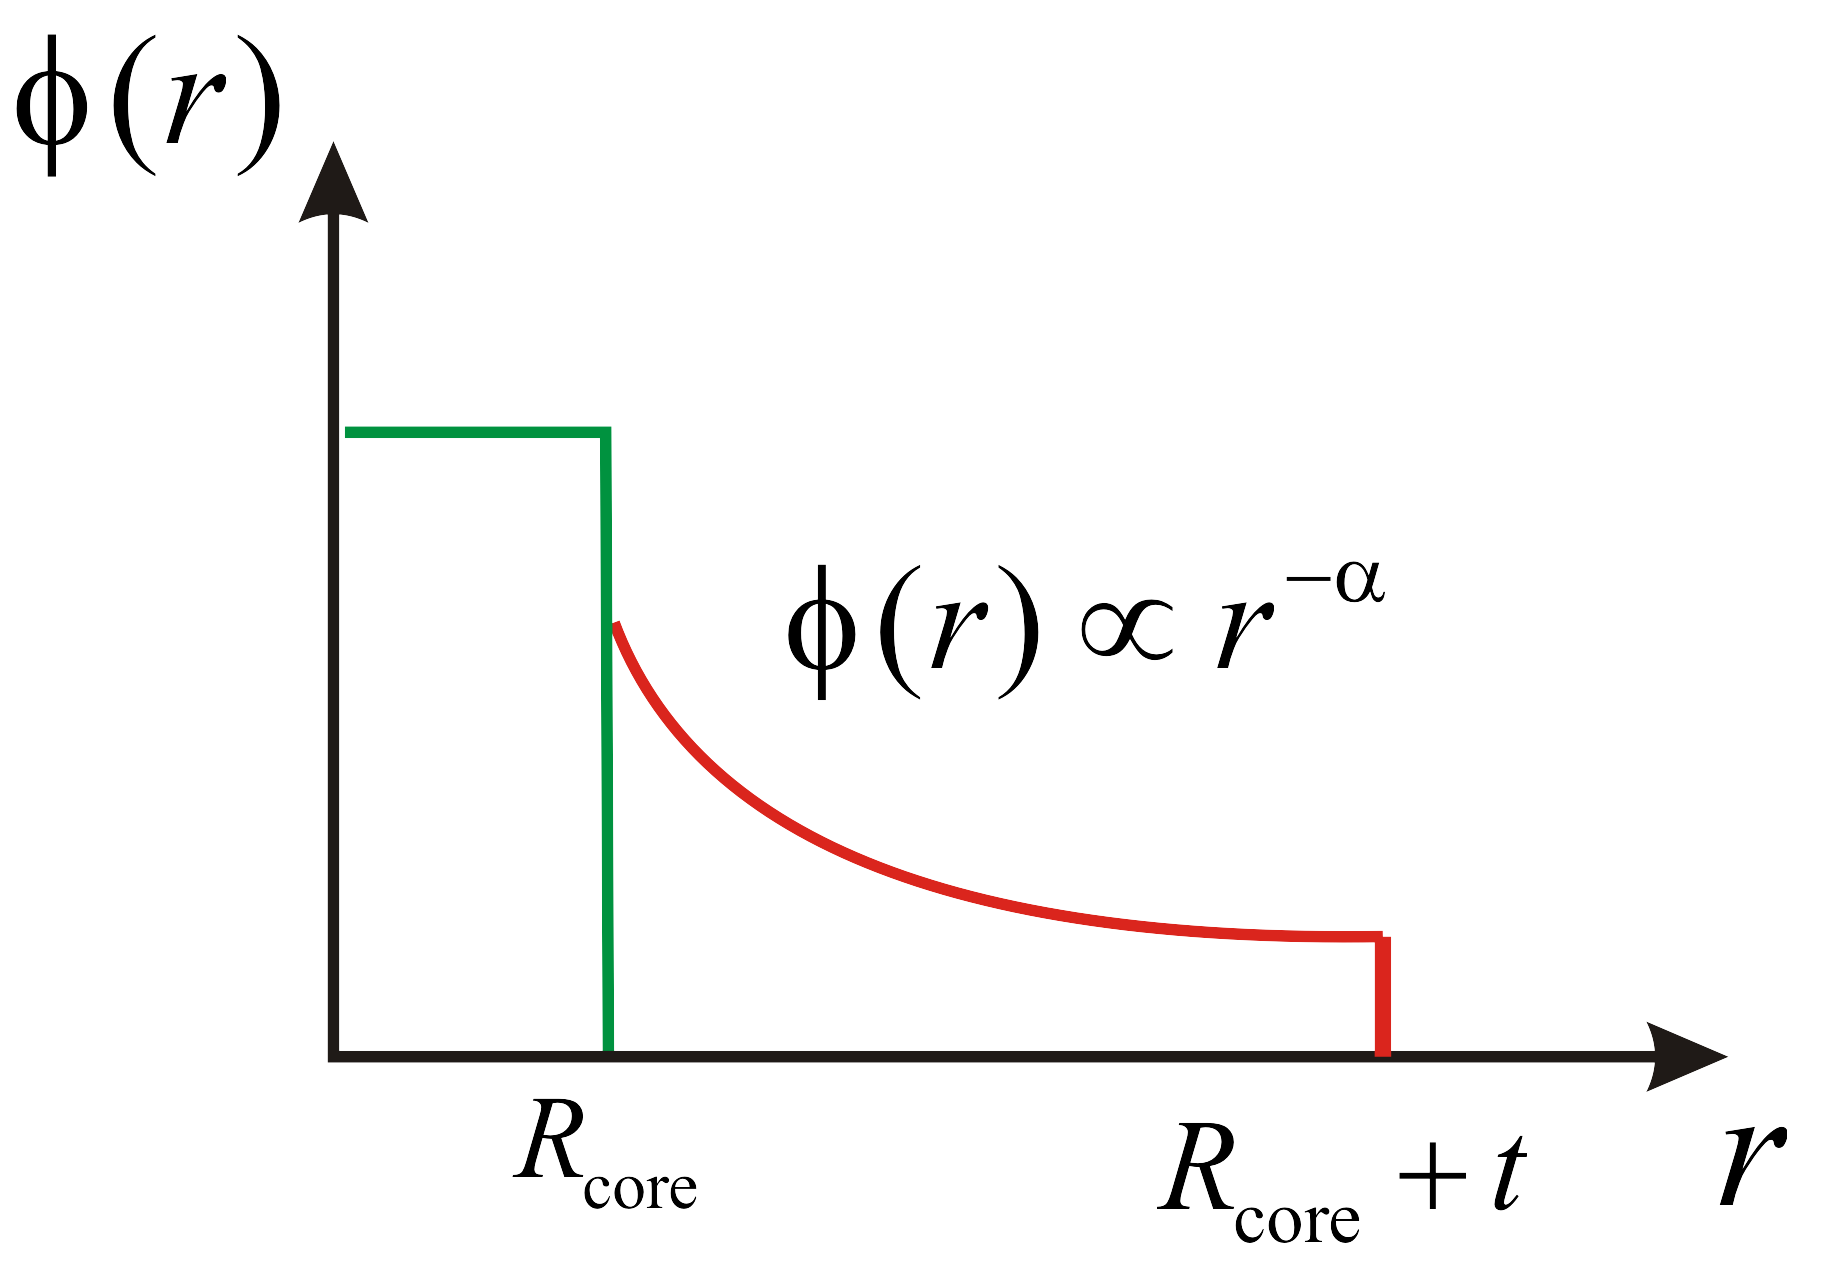
\includegraphics[width=0.55\textwidth,height=0.35\textwidth]{R_ma.png}
\end{center}
\caption{radial profile.}
\label{R_ma_profile}
\end{figure}

The structure of block copolymer micelles may be described in terms
of the model of starlike polymer as proposed by Daoud and Cotton
\cite{DaoudCotton82}. Starlike polymers consist of a homogeneous,
dense polymer core surrounded by a polymer layer. As a consequence
of the spherical or cylindrical geometry, the density profile
$\phi(r)$ in the polymer layer decreases according to Wijmans \&
Zhulina \cite{Wijmans93} as
\begin{align}
\phi(r)
\begin{cases}
\phi_\text{core}    & \text{for~} r < R_\text{core} \\
\phi_\text{brush} \left(\frac{r}{R_\text{core}}\right)^{-\alpha}
                    & \text{for~} R_\text{core} \leq r \leq R_\text{core}+t \\
 0                  & \text{for~} r > R_\text{core}+t
\end{cases}
\label{eq:R_ma_profile}
\end{align}
with $\alpha =(D-1)(3\nu-1)/(2\nu)$.
$D$ is determined by the dimension of the curvature of the grafted surface
(spherical $D=3$, cylindrical $D=2$, planar $D=1$).
$\nu$ is the Flory exponent, which has characteristic
values as given in Table \ref{FloryExp}.
The corresponding density profile is schematically
shown in Figure \ref{R_ma_profile}. Micelles consist of a well-defined
micellar core with a radius $R_\text{core}$ and a micellar shell or
corona extending to the outer micellar radius $R_m=R_\text{core}+t$,
where $t$ is the thickness of the corona.

\begin{table}[htb]
\caption{Flory exponent $\nu$ and exponent $\alpha$ of the radial
density profile for different thermodynamic states of
the polymer chains}
\label{FloryExp}
\begin{tabular}{ccccl}
  \hline
  % after \\: \hline or \cline{col1-col2} \cline{col3-col4} ...
  $\nu$ & $\alpha_\text{sphere}$& $\alpha_\text{cylinder}$ & $\alpha_\text{planar}$& \hspace{5mm}remarks \\
        & $D=3$                 & $D=2$                    & $D=1$                 & \\
  \hline
  & & & & \\
  1/3 & 0   & 0   & 0 & collapsed polymer \\
  1/2 & 1   & 1/2 & 0 & polymer in $\Theta$-solvent, semi-dilute solution \\
  3/5 & 4/3 & 2/3 & 0 & polymer in good solvent \\
  1   & 2   & 1   & 0 & polymer in stretched conformation,  e.g. polyelectrolyte
\end{tabular}
\end{table}

For a given radial profile according to eq.\ \ref{eq:R_ma_profile} the form factor of
spherical micelle can be calculated by
\begin{align}
F_\text{SPHERE} &= \int_0^\infty 2\pi r^2 \phi(r) \frac{\sin(qr)}{qr}\,dr
\end{align}
In case of a rod-like micelle the form factor can be separated in two terms
$I(q) = P_H(q)P_\text{cs}(q)$ as already in shown in eq.\ \ref{eq:rodlikeFF}.
The cross-term contribution to the scattering intensity is given by
\begin{align}
\begin{split}
P_\text{cs}(q) &=  F_\text{cs}^2(q) \\
F_\text{cs}(q) &=  \int_0^\infty 2\pi r \phi(r) J_0(q)\,dr
\end{split}
\end{align}
However, as it is more convenient here to formulate the scattering intensity in
terms of excess scattering length of the block units in the core $\beta_\text{core}$
and the corona $\beta_\text{brush}$ like in eq.\ \ref{eq:micelle} the form factor
is split into two parts, the form factor of the homogeneous core $F_\text{core}(q)$ and
the form factor of the corona $F_\text{brush}(q)$. The overall scattering intensity $I(q)$
is than given by
\begin{align}
\begin{split}
I(q) &=   N_\text{agg}^2\beta_\text{core}^2 F_\text{core}^2(q)
       + 2 N_\text{agg}^2\beta_\text{core}\beta_\text{corona} F_\text{core}(q) F_\text{corona}(q) \\
     & +   N_\text{agg}(N_\text{agg}-1) \beta_\text{corona}^2 F_\text{corona}^2(q)
       +   N_\text{agg} P_\text{brush}(q)
\end{split}
\label{masterR_ma}
\end{align}
The excess scattering length of a block in the corona and in the core, respectively,
$\beta_\text{brush}=V_\text{brush}(\eta_\text{brush}-\eta_\text{solv})$
and $\beta_\text{core}=V_\text{core}(\eta_\text{core}-\eta_\text{solv})$ are
defined in the same way than in eq.\ \ref{eq:micelle}.
$V_\text{brush}$ and $V_\text{core}$ are the total volume of a block in the corona
and in the core. $\eta_\text{brush}$ and $\eta_\text{core}$ are the corresponding
scattering length densities and $\eta_\text{solv}$ is the scattering length
density of the surrounding solvent. $F_\text{core}(q)$ is the form factor of the core and
normalized to 1 for $q=0$. Also the form factor of the corona $F_\text{corona}(q)$ and the
form factor of the local fluctuations in the corona originating from the individual chains
$P_\text{brush}(q)$ are normalized to 1 for $q=0$. Similar to section \ref{Chains(RW)}
models for spherical and rod-like shapes have been implemented which are described in the
following paragraphs.


\vspace{5mm}

\noindent
\subsubsection{\bf spherical core:}
\label{sect:SPHERE+R_ma}~\\

\begin{align}
F_\text{core}(q,R) &= 3\frac{\sin(qR)-qR\cos(qR)}{(qR)^3}
\end{align}
\begin{align}
F_\text{brush}(q,R,t)&= \frac{1}{C_{norm}}
   \int_{R_\text{core}}^{R_\text{core}+t} 2\pi r^2 r^{-\alpha} \frac{\sin(qr)}{qr} \, dr
\end{align}
with
\begin{align}
C_{norm} &=
\begin{cases}
\frac{4}{3-\alpha} \pi \left(\left(R_\text{core}+t\right)^{3-\alpha} - R_\text{core}^{3-\alpha}\right)
& \text{for~} \alpha \neq 2 \\
4\pi\ln\left(\frac{R_\text{core}+t}{R_\text{core}}\right)
& \text{for~} \alpha = 2
\end{cases} \nonumber
\end{align}
For the scattering contribution of the individual chains in the corona
$P_\text{brush}$ the scattering function for worm-like chains with excluded
volume and negligible cross-section, contour length $L$ and Kuhn-length $b$
according to section \ref{sect:WormLikeChain} has been implemented.

For micelles with a spherical core a few different parameterizations have been
implemented \texttt{SPHERE+R$\hat{~}$-a}, \texttt{SPHERE+R$\hat{~}$-a\_Rc} and
\texttt{SPHERE+R$\hat{~}$-a\_Nagg}.

\vspace{3mm}

\noindent
The parameters they all have in common are:
\begin{description}
\item[$V_\text{brush}$] molecular volume the diblock copolymer part forming the corona
\item[$\eta_\text{core}$] scattering length density of the diblock copolymer part forming the core
\item[$\eta_\text{brush}$] scattering length density of the diblock copolymer part forming the corona
\item[$\eta_\text{solv}$] scattering length density of the solvent
\item[$\alpha$] exponent of the radial scattering length density profile ($r^{-\alpha}$)
\item[$t$] corona thickness
\item[$L$] contour length of the chain in the corona
\item[$b$] Kuhn-length of the chain in the corona
\end{description}

\vspace{3mm}
\noindent
For the model \texttt{SPHERE+R$\hat{~}$-a} the other parameters are
\begin{description}
\item[$R_\text{core}$] radius of the micellar core
\item[$n_\text{agg}$] grafting density (number of copolymer molecules
$N_\text{agg}$ per surface are $S$, $n_\text{agg}=N_\text{agg}/S$)
\end{description}

\noindent
In contrast to the form factor \texttt{SPHERE+R$\hat{~}$-a\_Rc} and \texttt{SPHERE+R$\hat{~}$-a\_Nagg}
this one does not necessary consist of copolymers.
The excess scattering lengths and aggregation number are given by
\begin{align}
N_\text{agg} &= n_\text{agg} S
\end{align}
where the surface of the core is given by $S=4\pi R_\text{core}^2$. Together with the
core volume  $V =\frac{4}{3}\pi R_\text{core}^3$ one gets for the excess scattering
lengths
\begin{align}
\beta_\text{core} &= \frac{V (1-x_\text{solv,core})}{N_\text{agg}}
(\eta_\text{core}-\eta_\text{solv}) \\
\beta_\text{brush} &= V_\text{brush} (\eta_\text{brush}-\eta_\text{solv})
\end{align}

\vspace{3mm}

\hspace{1pt}\\
\underline{Input Parameters for model \texttt{SPHERE+R$\hat{~}$-a}:}
\begin{description}
\item[\texttt{R\_core}] core radius
\item[\texttt{n\_agg}] specific aggregation number (number of chains per surface area)
\item[\texttt{V\_brush}]  molecular volume of a block unit in the micellar corona
\item[\texttt{eta\_core}] scattering length density of spherical core
\item[\texttt{eta\_brush}] scattering length density of the block unit in the corona
\item[\texttt{eta\_solv}] scattering length density of solvent
\item[\texttt{alpha}] exponent of the radial scattering length density profile ($r^{-\alpha}$)
\item[\texttt{t}] corona thickness
\item[\texttt{L}] contour length of the chain in the corona
\item[\texttt{b}] Kuhn-length of the chain in the corona
\end{description}

\clearpage

\noindent
For the model \texttt{SPHERE+R$\hat{~}$-a\_Rc} the other parameters are
\begin{description}
\item[$R_\text{core}$] core radius
\item[$V_\text{core}$] molecular volume of single block unit in the micellar core
\end{description}
The excess scattering lengths and aggregation number for eq.\
\ref{eq:micelle} are given by
\begin{align}
\beta_\text{core}  &= V_\text{core}  (\eta_\text{core} -\eta_\text{solv}) \\
\beta_\text{brush} &= V_\text{brush} (\eta_\text{brush}-\eta_\text{solv}) \\
N_\text{agg} &= (1-x_\text{solv,core}) \frac{4}{3}\pi R_\text{core}^3  / V_\text{core}
\end{align}

\hspace{1pt}\\
\underline{Input Parameters for model \texttt{SPHERE+R$\hat{~}$-a\_Rc}:}
\begin{description}
\item[\texttt{R\_core}] core radius
\item[\texttt{V\_core}] molecular volume of single block unit in the micellar core
\item[\texttt{V\_brush}]  molecular volume of single block unit in the micellar corona
\item[\texttt{eta\_core}] scattering length density of spherical core
\item[\texttt{eta\_brush}] scattering length density of the block unit in the corona
\item[\texttt{eta\_solv}] scattering length density of solvent
\item[\texttt{alpha}] exponent of the radial scattering length density profile ($r^{-\alpha}$)
\item[\texttt{t}] corona thickness
\item[\texttt{L}] contour length of the chain in the corona
\item[\texttt{b}] Kuhn-length of the chain in the corona
\end{description}

\vspace{10mm}

\noindent
For the model \texttt{SPHERE+R$\hat{~}$-a\_Nagg} the other parameters are
\begin{description}
\item[$N_\text{agg}$] aggregation number
\item[$V_\text{core}$] molecular volume of single block unit in the micellar core
\end{description}
The excess scattering lengths and the core radius $R_\text{core}$ needed for eq.\
\ref{eq:micelle} are given by
\begin{align}
\beta_\text{core}  &= V_\text{core}  (\eta_\text{core} -\eta_\text{solv}) \\
\beta_\text{brush} &= V_\text{brush} (\eta_\text{brush}-\eta_\text{solv}) \\
R_\text{core} &= \left( \frac{N_\text{agg} V_\text{core}}{1-x_\text{solv,core}}
                         \, \frac{3}{4\pi}\right)^{1/3}
\end{align}

\hspace{1pt}\\
\underline{Input Parameters for model \texttt{SPHERE+R$\hat{~}$-a\_Nagg}:}
\begin{description}
\item[\texttt{N\_agg}] aggregation number
\item[\texttt{V\_core}] molecular volume of single block unit in the micellar core
\item[\texttt{V\_brush}]  molecular volume of single block unit in the micellar corona
\item[\texttt{eta\_core}] scattering length density of spherical core
\item[\texttt{eta\_brush}] scattering length density of the block unit in the corona
\item[\texttt{eta\_solv}] scattering length density of solvent
\item[\texttt{alpha}] exponent of the radial scattering length density profile ($r^{-\alpha}$)
\item[\texttt{t}] corona thickness
\item[\texttt{L}] contour length of the chain in the corona
\item[\texttt{b}] Kuhn-length of the chain in the corona
\end{description}





\vspace{5mm}

\noindent
\subsubsection{\bf rodlike core:}
\label{sect:ROD+R_ma}~\\
In case of a rod-like micelle the form factor can be separated in two terms $I(q) =
P_H(q)P_\text{cs}(q)$ as already in shown in eq. \ref{eq:rodlikeFF}. The cross-term contribution to the scattering
intensity is given by
\begin{align}
\begin{split}
P_\text{cs}(q) &=  F_\text{cs}^2(q) \\
F_\text{cs}(q) &= \int_0^\infty 2\pi r \phi(r) J_0(qr)\,dr
                = F_\text{cs,core}(q)+F_\text{cs,brush}(q)
\end{split}
\end{align}
The contribution of the homogeneous core is given by
\begin{align}
F_\text{cs,core}(q) = \frac{2 J_1(qR_c)}{qR_c}
\end{align}
and for the corona by
\begin{align}
F_\text{cs,brush}(q) &=\frac{1}{c_\alpha}\int_{R_c}^{R_c+t} 2\pi r \, r^{-\alpha} J_0(qr)\,dr
\end{align}
\begin{align}
c_\alpha &= \int_{R_c}^{R_c+t} 2\pi r \, r^{-\alpha}\,dr \nonumber \\
&= \begin{cases}
2\pi\ln\left(\frac{R_c+t}{R_c}\right)                                   & \text{~for~} \alpha = 2   \\
\frac{2}{2-\alpha} \pi \left((R_c+t)^{2-\alpha}-R_c^{2-\alpha}\right)   & \text{~for~} \alpha \neq 2
\end{cases}
\end{align}

For the scattering contribution of the individual chains in the corona $P_\text{local}$ normally
can be neglected for rod-like micelles in contrast to spherical structures as for structures
with a lower dimension than spheres, this contribution becomes more and more negligible. To account
for the scattering of the individual chains at least in first approximation and without introducing
new parameters a form factor similar to the one of star polymers has been implemented.
\begin{align}
P_\text{local}(q) &=
             \frac{\Gamma(\mu)}{qt}
             \frac{\sin\left(\mu \arctan(q t)\right)}{\left(1+q^2t^2\right)^{\mu/2}} \\
\mu &=\frac{1}{\nu}-1 ,\quad
\alpha = \frac{3\nu-1}{2\nu} \quad
\Leftrightarrow \quad \mu = 2(1-\alpha) \nonumber
\end{align}
The form factor to describe the scattering of the individual chains
is identical to the blob scattering contribution in star-like polymers according to
Dozier (\ref{sect:DozierStar}). The exponential damping length $\xi$ in the definition of the star
polymer has been set to the shell thickness $t$. In the original
paper of Pedersen the $P_\text{local}$ was described by the scattering of a semi-flexible chain with
excluded volume according to section \ref{sect:WormLikeChain}, which however would require to define
two more parameters.

For micelles with a rod-like core a few different parameterizations have been
implemented \texttt{ROD+R$\hat{~}$-a}, \texttt{ROD+R$\hat{~}$-a\_Rc} and
\texttt{ROD+R$\hat{~}$-a\_Nagg}.

\vspace{3mm}

\noindent
The parameters they all have in common are:
\begin{description}
\item[$V_\text{brush}$] molecular volume the diblock copolymer part forming the corona
\item[$\eta_\text{core}$] scattering length density of the diblock copolymer part forming the core
\item[$\eta_\text{brush}$] scattering length density of the diblock copolymer part forming the corona
\item[$\eta_\text{solv}$] scattering length density of the solvent
\item[$x_\text{solv,core}$] amount of solvent in the core
\item[$\alpha$] exponent of the radial scattering length density profile ($r^{-\alpha}$)
\item[$t$] corona thickness
\item[$H$] height of the cylinder
\end{description}

\vspace{3mm}
\noindent
For the model \texttt{ROD+R$\hat{~}$-a} the other parameters are
\begin{description}
\item[$R_\text{core}$] radius of the micellar core
\item[$n_\text{agg}$] grafting density (number of copolymer molecules
$N_\text{agg}$ per surface are $S$, $n_\text{agg}=N_\text{agg}/S$)
\end{description}

\noindent
In contrast to the form factor \texttt{ROD+R$\hat{~}$-a\_Rc} and \texttt{ROD+R$\hat{~}$-a\_Nagg}
this one does not necessary consist of copolymers.
The excess scattering lengths and aggregation number are given by
\begin{align}
N_\text{agg} &= n_\text{agg} S
\end{align}
where the surface of the core is given by $S=2\pi R_\text{core}H$. Together with the
core volume  $V =\pi R_\text{core}^2H$ one gets for the excess scattering
lengths
\begin{align}
\beta_\text{core} &= \frac{V_\text{core} (1-x_\text{solv,core})}{N_\text{agg}}
(\eta_\text{core}-\eta_\text{solv}) \\
\beta_\text{brush} &= V_\text{brush} (\eta_\text{brush}-\eta_\text{solv})
\end{align}

\vspace{3mm}

\hspace{1pt}\\
\underline{Input Parameters for model \texttt{ROD+R$\hat{~}$-a}:}
\begin{description}
\item[\texttt{R\_core}] core radius
\item[\texttt{n\_agg}] specific aggregation number (number of chains per surface area)
\item[\texttt{V\_brush}]  molecular volume of a block unit in the micellar corona
\item[\texttt{eta\_core}] scattering length density of spherical core
\item[\texttt{eta\_brush}] scattering length density of the block unit in the corona
\item[\texttt{eta\_solv}] scattering length density of solvent
\item[\texttt{xsolv\_core}] amount of solvent in the core
\item[\texttt{alpha}] exponent of the radial scattering length density profile ($r^{-\alpha}$)
\item[\texttt{t}] corona thickness
\item[\texttt{H}] rod height
\end{description}


\vspace{3mm}
\noindent
For the model \texttt{ROD+R$\hat{~}$-a\_Rc} the other parameters are
\begin{description}
\item[$R_\text{core}$] core radius
\item[$V_\text{core}$] molecular volume of single block unit in the micellar core
\end{description}
The excess scattering lengths and aggregation number for eq.\
\ref{eq:micelle} are given by
\begin{align}
\beta_\text{core}  &= V_\text{core}  (\eta_\text{core} -\eta_\text{solv}) \\
\beta_\text{brush} &= V_\text{brush} (\eta_\text{brush}-\eta_\text{solv}) \\
N_\text{agg} &=  2\pi R_\text{core}^2H   \, \frac{1-x_\text{solv,core}}{V_\text{core}}
\end{align}

\hspace{1pt}\\
\underline{Input Parameters for model \texttt{ROD+R$\hat{~}$-a\_Rc}:}
\begin{description}
\item[\texttt{R\_core}] core radius
\item[\texttt{V\_core}] molecular volume of single block unit in the micellar core
\item[\texttt{V\_brush}]  molecular volume of single block unit in the micellar corona
\item[\texttt{eta\_core}] scattering length density of spherical core
\item[\texttt{eta\_brush}] scattering length density of the block unit in the corona
\item[\texttt{eta\_solv}] scattering length density of solvent
\item[\texttt{xsolv\_core}] amount of solvent in the core
\item[\texttt{alpha}] exponent of the radial scattering length density profile ($r^{-\alpha}$)
\item[\texttt{t}] corona thickness
\item[\texttt{H}] rod height
\end{description}

\vspace{10mm}

\noindent
For the model \texttt{ROD+R$\hat{~}$-a\_Nagg} the other parameters are
\begin{description}
\item[$n_\text{agg}$] specific aggregation number, aggregation number per surface area
\item[$V_\text{core}$] molecular volume of single block unit in the micellar core
\end{description}
The excess scattering lengths and the core radius $R_\text{core}$ needed for eq.\
\ref{eq:micelle} are given by
\begin{align}
\beta_\text{core}  &= V_\text{core}  (\eta_\text{core} -\eta_\text{solv}) \\
\beta_\text{brush} &= V_\text{brush} (\eta_\text{brush}-\eta_\text{solv}) \\
R_\text{core} &=  \frac{2 n_\text{agg}\, V_\text{core}}{1-x_\text{solv,core}}
\end{align}

\hspace{1pt}\\
\underline{Input Parameters for model \texttt{ROD+R$\hat{~}$-a\_nagg}:}
\begin{description}
\item[\texttt{n\_agg}] specific aggregation number (number of chains per surface area)
\item[\texttt{V\_core}] molecular volume of single block unit in the micellar core
\item[\texttt{V\_brush}]  molecular volume of single block unit in the micellar corona
\item[\texttt{eta\_core}] scattering length density of spherical core
\item[\texttt{eta\_brush}] scattering length density of the block unit in the corona
\item[\texttt{eta\_solv}] scattering length density of solvent
\item[\texttt{xsolv\_core}] amount of solvent in the core
\item[\texttt{alpha}] exponent of the radial scattering length density profile ($r^{-\alpha}$)
\item[\texttt{t}] corona thickness
\item[\texttt{H}] rod height
\end{description}

\noindent
REFERENCES:\\
\cite{DaoudCotton82,FoersterHermsdorf2002,MuellerDelsanti2000,Wijmans93}
%\begin{enumerate}
%\item M. Daoud and J.P. Cotton,
%Star shaped polymers - A model for the conformation and its concentration-dependence
%Journal de Physique (Paris) 1982, 43, 531.
%\item S. F\"orster,  N. Hermsdorf, C. B\"ottcher and P. Lindner,
%Structure of Polyelectrolyte Block Copolymer Micelles,
%Macromolecules 2002, 35, 4096-4105
%\item F. M\"uller, M. Delsanti, L. Auvray, J. Yang, Y.J. Chen, J.W. Mays,
%B. Dem�, M. Tirrell, and P. Guenoun, Ordering of urchin-like charged
%copolymer micelles: Electrostatic, packing and polyelectrolyte
%correlations, Eur. Phys. J. E 3, 45�53 (2000)
%\item C. M. Wijmans and E. B. Zhulina,
%Polymer Brushes at Curved Surfaces,
%Macromolecules 1993,26,1214-7224
%\end{enumerate}


\clearpage
\subsubsection{spherical Micelles with a homogeneous core
and a corona of semi-flexible interacting self-avoiding chains}~\\

\subsection{Sphere with Gaussian chains attached} ~\\
\begin{figure}[htb]
\begin{center}
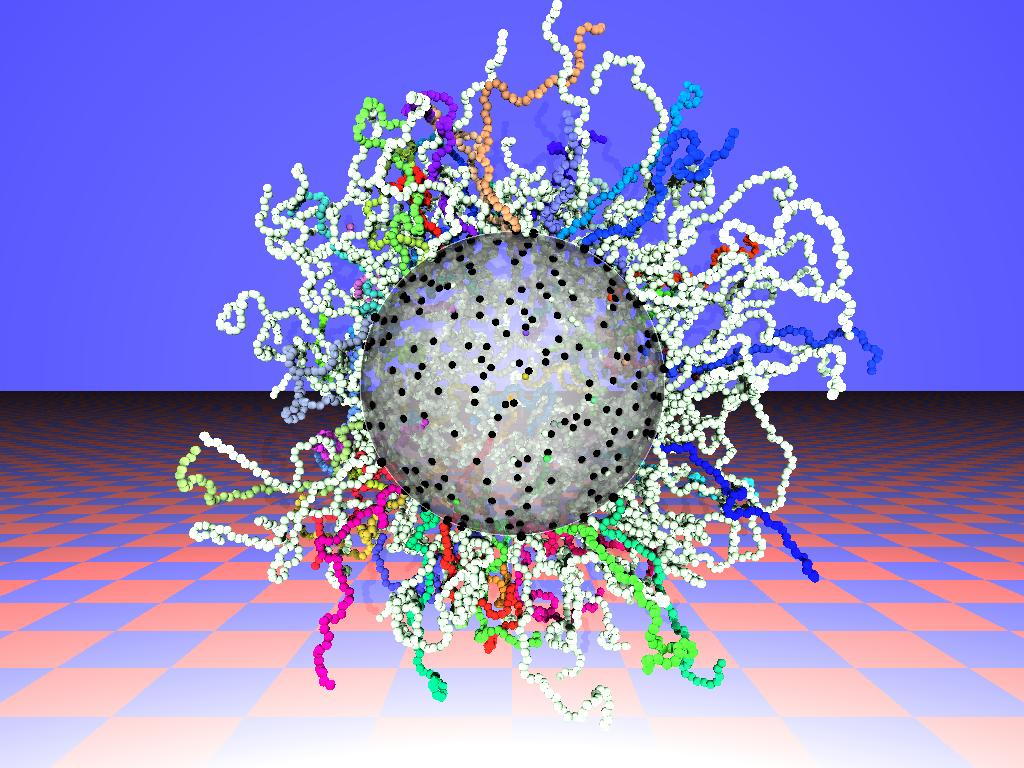
\includegraphics[width=0.75\textwidth,height=0.55\textwidth]{agghalf.png}
\end{center}
\caption{Block copolymer micelles.}
\label{SphereWithGaussChains}
\end{figure}

The expressions have been derived by Pedersen and Gerstenberg
\cite{PedersenGerstenberg96,PedersenJApplCryst2000}. For a sphere with radius $R$ and total excess scattering
length $\rho_s$ with $N_\text{agg}$ attached chains
\begin{align}
P_{mic}(Q) & = N_\text{agg}^2 \rho_s^2 P_s(Q,R) + N_{agg} \rho_c^2 P_c(Q,R_g) \\
           & + N_\text{agg}(N_{agg}-1)\rho_c^2  S_{cc}(Q)
             + 2N_\text{agg}^2 \rho_s \rho_c S_{sc}(Q) \nonumber
\end{align}
with:
\begin{align}
P_s &= \Phi^2(Q,R) \\
\Phi(Q,R) &= 3 \frac{\sin(QR)-QR\cos(QR)}{(QR)^3} \\
P_c(Q,R_g) &= 2 \frac{\exp(-x)-1+x}{x^2} \\
x &= R_g^2Q^2 \\
\Psi(Q,R_g) &= \frac{1-\exp(-x)}{x} \\
S_\text{cc}(Q) &= \Psi^2(Q, R_g) \left(\frac{\sin(Q(R+d\,\,R_g))}{Q(R+d\,R_g)}\right)^2 \\
S_\text{sc}(Q) &= \Psi(Q, R_g)\Phi(Q R_g)\frac{\sin(Q(R+d\,R_g))}{Q(R+d\,R_g)}
\end{align}
where $R_g$ is the root-mean-square radius of
gyration of a chain. $\rho_c$ is the total excess scattering length of a single chain.
Non-penetrating of the chains into the core region is mimicked by $d\approx 1$ for $R\gg R_g$.

\vspace{5mm}

\hspace{1pt}\\
\underline{Input Parameters for model \texttt{SphereWithGaussChains}:}\\
\begin{description}
\item[\texttt{R}] radius of core $R$
\item[\texttt{Rg}] gyration radius of chain $R_g$
\item[\texttt{d}] for non-penetration of the chains into the core region $d\approx 1$.
\item[\texttt{Nagg}] aggregation number $N_\text{agg}$
\item[\texttt{rc}] excess scattering length of a block in the chains $\rho_c$
\item[\texttt{rs}] excess scattering length of a block in the core $\rho_s$
\end{description}

\vspace{5mm}

%\noindent REFERENCE:\\
%Pedersen, J.S. and Gerstenberg, M.C., Macromolecules 1996 (29) 1363-1365\\
%J. S. Pedersen,
%Form factors of block copolymer micelles with spherical, ellipsoidal and cylindrical cores,
%J. Appl. Cryst. (2000). 33, 637-640

%%%%%%%%%%%%%%%%%%%%%%%%%%%%%%%%%%%%%%%%%%%%%%%%%%%%%%%%%%%%%%%%%%%%%%%%%

\clearpage
\subsection{Sphere with Gaussian chains attached (block copolymer micelle)} ~\\

This form factor is the same than for \texttt{SphereWithGaussChains}. It has only been slightly re-parametrised.
Instead of the core radius $R$ and excess scattering lengths $\rho_s$ and $\rho_c$  the
volumes $V_\text{polym,c}$ and $V_\text{polym,sh}$ of the block units building the core and the shell are required
together with the corresponding scattering length densities $\eta_\text{poly,c}$, $\eta_\text{poly,sh}$ and
that one of the solvent $\eta_\text{solv}$. Furthermore $x_\text{solv,c}$ is the amount of solvent in the core which
takes account for a possible swelling of the core. These parameters allow one to calculate the core radius and
excess scattering lengths by
\begin{align}
    R &= \left(\abs{ \frac{N_\text{agg}V_\text{polym,c}}{1-x_\text{solv,c}}} \frac{3}{4\pi}\right)^{1/3}   \\
    \rho_s &= V_\text{polym,c} \left(\eta_\text{poly,c}-\eta_\text{solv} \right) \\
    \rho_c &= V_\text{polym,sh} \left(\eta_\text{poly,sh}-\eta_\text{solv}\right)
\end{align}

The volumes $V_\text{polym,c}$ and $V_\text{polym,sh}$ can be calculated by knowing the molecular weights\footnote{$u=1.660 538 86 \times 10^{-27}$ kg}
of the block units of the polymer in the core $M_\text{polym,c}$ and in the shell $M_\text{polym,sh}$ together
with their bulk mass densities $\rho_\text{polym,c}$ and $\rho_\text{polym,sh}$. The volumes are then
given by
\begin{align}
V_\text{polym,c} = \frac{M_\text{polym,c}}{N_a\, \rho_\text{polym,c}}
\quad \text{ and } \quad
V_\text{polym,sh} = \frac{M_\text{polym,sh}}{N_a\, \rho_\text{polym,sh}}
\end{align}
whereby $N_a$ is Avogadro's constant\footnote{$N_a = 6.022 1415 \times 10^{23} \text{mol}^{-1}$}. The units of the block units
has to be supplied in units corresponding to the scattering vector $Q$, i.e. in nm$^3$ in case $Q$ is given in nm$^{-1}$
or in \AA$^3$ in case $Q$ is given in \AA$^{-1}$.
\vspace{5mm}

\hspace{1pt}\\
\underline{Input Parameters for model \texttt{BlockCopolymerMicelle}:}\\
\begin{description}
\item[\texttt{Vpolym\_c}] volume of a single block unit of the chains in the core $V_\text{polym,c}$,
     it should be given in units of nm$^3$ in case $Q$ is given in nm$^{-1}$ and in units of \AA$^3$
     in case $Q$ is given in \AA$^{-1}$.
\item[\texttt{xsolv\_c}] amount of solvent in the core ($x_\text{solv,c}\neq 1$)
\item[\texttt{Vpolym\_sh}] volume of a single block unit of the chains in the shell $V_\text{polym,sh}$,
     it should be given in units of nm$^3$ in case $Q$ is given in nm$^{-1}$ and in units of \AA$^3$
     in case $Q$ is given in \AA$^{-1}$.
\item[\texttt{eta\_poly\_c}] scattering length density of the block units in the core $\eta_\text{c}$
\item[\texttt{eta\_poly\_sh}] scattering length density of the block units in the chains $\eta_\text{sh}$
\item[\texttt{eta\_solv}] scattering length density of the solvent $\eta_\text{solv}$
\item[\texttt{Nagg}] aggregation number $N_\text{agg}$
\item[\texttt{Rg}] gyration radius of chain $R_g$
\item[\texttt{d}] for non-penetration of the chains into the core region $d\approx 1$.
\end{description}
